
\section*{Original Experiments and Technical Details}

\section{Detailed Related Work and Positioning}
\label{sec:related_work}

\paragraph{Typed graph representations.}
Cartesian Genetic Programming (CGP) represents programs as graphs with reusable intermediate values~\cite{miller2015cartesian}. Mixed Type CGP (MT-CGP) extends this representation to multiple data types~\cite{harding2012mtcgp}; typed program graphs are therefore an established foundation. Strongly typed GP~\cite{montana1995strongly} likewise uses declared interfaces to constrain valid compositions. AdaptoFlux builds on these ideas with a common registration and execution interface for heterogeneous host-language callables, including external-state operations, together with interchangeable search procedures and reusable graph modules.

\paragraph{Data dependencies and effect ordering.}
LLVM's SelectionDAG explicitly distinguishes typed data values from chain dependencies that order side-effecting operations such as memory accesses and calls~\cite{llvmSelectionDAG}. The separation of data flow from effect order is established compiler practice. AdaptoFlux applies this principle to an executable symbolic-synthesis substrate: data edges bind callable arguments, while a saved execution plan orders declared conflicting resource accesses. Its operators may invoke application environments rather than target-machine instructions. The implementation maintains the execution contract through candidate evaluation, graph edits, extraction, and model persistence (Appendix~\ref{app:revision_effects}).

\paragraph{Functional abstraction and explicit state.}
DreamCoder~\cite{ellis2021dreamcoder} learns reusable abstractions within a functional program space. Mutable interaction can also be expressed functionally by passing state values through a program. AdaptoFlux offers an interface in which registered methods access external state directly. The paired translation in Appendix~\ref{app:revision_encoding} makes the relation concrete: explicit state edges and implicit accesses reproduce the same tested trajectories when their access order agrees. This is a choice of programming interface and execution contract, rather than a separation in computability. DreamCoder's library-learning method and AdaptoFlux's graph-extraction procedure address related reuse goals with different search mechanisms.

\paragraph{Constraint-guided synthesis.}
Popper~\cite{cropper2021learning} learns logical programs using a generate--test--constrain loop. Declared types in AdaptoFlux similarly restrict which compositions a search examines. Popper additionally derives constraints from failed hypotheses, whereas the current AdaptoFlux filters are supplied through type declarations and search metadata. Logical relations, explicit state arguments, and external-state callables provide different interfaces for representing transitions. The comparisons concern these interfaces and their execution, rather than an impossibility of expressing transitions in a logical language.

\paragraph{Symbolic regression and policy search.}
PySR~\cite{cranmer2023interpretable}, gplearn and AI Feynman~\cite{udrescu2020ai} provide specialized procedures for recovering numerical expressions. Risk-seeking policy-gradient methods learn distributions over symbolic expressions~\cite{petersen2019deep}, including control policies~\cite{landajuela2021discovering}, while language-model-guided discovery combines proposals with systematic evaluation~\cite{romera2024mathematical}. These methods emphasize search quality. AdaptoFlux supplies operator registration, graph construction and execution facilities that can host different optimizers; the CMA-trained controller in Appendix~\ref{app:revision_action} illustrates this separation. The static comparisons in Appendix~\ref{sec:appendix_baseline_comparison} report the behavior of the tested restricted method pools and probes.

\paragraph{State feedback and contribution.}
Repeated evaluation connects an acyclic stored graph to a changing environment. This organization is compatible with classical feedback systems~\cite{wiener1948cybernetics,ashby1960brain} and with explicit state-threading representations. The contribution is an integrated, inspectable substrate combining heterogeneous typed callables, persistent state-order contracts, graph reuse, and optimizer-independent evaluation. Its empirical support spans controlled type-prior comparisons, paired state encodings, structured action programs and execution-scale measurements.

\section{Complete Derivation of AdaptoFlux Inference and Training Complexity}
\label{sec:complexity_analysis}

\paragraph{Implementation version.}
The cost decomposition below describes the original execution backend used by the historical experiments and the controlled measurements in Appendix~\ref{app:revision_scaling}. The revised executor additionally prepares a persistent semantic order and effect-control dependencies (Appendix~\ref{app:revision_effects}). Its preparation cost depends on the graph and declared resource accesses; the original timing measurements do not include that new pass. Scheduling operates on the union of data and control dependencies, and available parallelism is determined by this augmented graph.


This appendix provides a detailed derivation of the time and space complexity of the AdaptoFlux architecture during single inference, task-parallel inference, and under three main training strategies (LayerGrow, GraphEvo, CombinedTrainer).

\subsection{Symbol Definitions and Basic Assumptions}

To ensure consistency in the derivation, we first uniformly define general symbols, complexity constants, and basic assumptions.

\subsubsection{General Symbol Table}

\begin{table}[htbp]
    \centering
    \caption{General Symbols}
    \label{tab:symbols_general}
    \begin{tabular}{ll}
        \toprule
        \textbf{Symbol} & \textbf{Meaning} \\
        \midrule
        $N$ & Inference batch size (number of samples) \\
        $V$ & Number of computation graph nodes (excluding \texttt{root} and \texttt{collapse}) \\
        $E$ & Number of computation graph edges (explicit data dependencies) \\
        $D_{\mathrm{in}}$ & Input feature dimension \\
        $D_{\mathrm{out}}$ & Output feature dimension \\
        $W$ & Average graph width (maximum number of concurrent nodes) \\
        $L_{\mathrm{crit}}$ & Critical path length (longest data dependency chain) \\
        $P$ & Number of parallel scheduling threads/processes \\
        \bottomrule
    \end{tabular}
\end{table}

\textit{Note: The above parameters are highly dependent on specific task configurations, data scales, and graph topologies. The framework design does not make fixed prior assumptions about them.}

\subsubsection{Complexity Constant Dependency Characteristics}

\begin{table}[htbp]
    \centering
    \caption{Complexity Constants and Dependencies}
    \label{tab:constants}
    \begin{tabular}{lp{0.75\linewidth}}
        \toprule
        \textbf{Constant} & \textbf{Meaning and Dependency} \\
        \midrule
        $C_{\mathrm{copy}}$ & Python object reference extraction overhead. Fixed at $O(1)$ (nanosecond-level memory pointer operations), independent of graph scale. \\
        $C_{\mathrm{sync}}$ & Global lock acquisition/release and queue synchronization overhead. Fixed at $O(1)$ (microsecond-level OS primitives), potentially becoming a serial bottleneck under high concurrency. \\
        $\bar{C}_{\mathrm{op}}$ & \textbf{Average method computational complexity} (where $\mathrm{op}$ denotes the underlying \textbf{operation}). \textbf{Strongly depends on method pool composition}: Pure Python loops are constrained by interpreter overhead; C/Numba extensions can release the GIL to achieve true parallelism. This constant directly determines the absolute performance boundary of the framework. \\
        $\rho_{\mathrm{lock}}$ & Global lock contention factor. Dynamic range $[1/P, 1]$, actual value depends on graph width $W$, data flow topology, and thread scheduling strategy. \\
        \bottomrule
    \end{tabular}
\end{table}

\subsubsection{Basic Assumptions}

\textbf{Assumption 1 [Typical Deployment Scenario]} \\
In typical deployment scenarios, the following conditions are met:
\begin{enumerate}
    \item $N \gg V, E$ (Batch size is much larger than graph scale)
    \item $D_{\mathrm{in}}, D_{\mathrm{out}}$ are constants or independent of $N$
    \item $C_{\mathrm{copy}}, C_{\mathrm{sync}}$ are $O(1)$ constants
    \item Method library size $M$ is a bounded constant
    \item Search hyperparameters ($L, A, C, R, S, f$) are bounded constants
\end{enumerate}

\textbf{Assumption 2 [Operator Implementation]} \\
Operator implementations satisfy:
\begin{enumerate}
    \item Pure Python operators: $\bar{C}_{\mathrm{op}}$ includes significant interpreter overhead
    \item I/O or C extension operators: Can release GIL, supporting true parallelism
\end{enumerate}

\subsection{Inference Phase Complexity Analysis}

\subsubsection{Single Inference: Four-Stage Decomposition}
\label{sec:single_inference}

\textbf{Definition [Single Inference]} \\
Single inference refers to the process where the model, in deployment state, performs forward propagation on a given input batch to generate prediction results. In the AdaptoFlux architecture, the inference process is modeled as data flow execution on a Directed Acyclic Graph (DAG).

\paragraph{Stage 1: Input Normalization and Preprocessing}
The system first converts input data into an internal sample list structure. The complexity of this step depends on the input data type:
\begin{itemize}
    \item \textbf{Dense Numerical Matrix}: Involves memory copying and type checking, with complexity $O(N \cdot D_{\mathrm{in}})$
    \item \textbf{Complex Objects (dtype=object)}: Main overhead lies in reference counting and list construction, still maintaining a linear relationship $O(N \cdot D_{\mathrm{in}})$
\end{itemize}

\paragraph{Stage 2: Graph Topological Sorting}
To ensure correct node execution order dependencies, the system performs topological sorting on the computation graph. This operation depends only on the graph structure and is independent of the sample size $N$:
\begin{equation}
    T_{\mathrm{topo}} = O(V + E)
\end{equation}

\paragraph{Stage 3: Node Layer-by-Layer Execution}
This is the core computational part of the inference process. The system traverses each node $v \in \mathcal{V}$ in topological order. For each node, the following sub-operations are performed:

\begin{enumerate}
    \item \textbf{Edge Data Extraction}: Based on incoming edge configurations, feature data for $N$ samples is extracted from predecessor node outputs. The total number of incoming edges in the graph is $E$, and the data extraction complexity is:
    \begin{equation}
        T_{\mathrm{extract}} = O(E \cdot N \cdot C_{\mathrm{copy}})
    \end{equation}
    
    \item \textbf{Operator Computation}: Executes the computation method bound to the node. Let the single-sample computational complexity of node $v$ be $C_{\mathrm{op}}(v)$. If the method supports vectorization, $C_{\mathrm{op}}(v)$ approaches the efficiency of underlying kernel optimization; if it degrades to sample-by-sample loops, $C_{\mathrm{op}}(v)$ includes significant Python interpreter overhead.
    
    The total complexity of the node execution phase is:
    \begin{equation}
        T_{\mathrm{compute}} = O\left(N \cdot \sum_{v \in \mathcal{V}} C_{\mathrm{op}}(v)\right) = O(N \cdot V \cdot \bar{C}_{\mathrm{op}})
    \end{equation}
\end{enumerate}

\paragraph{Stage 4: Result Aggregation and Collapse}
The final stage of inference maps the outputs of specified nodes to global coordinates and performs collapse processing. This process requires traversing the final feature vectors of $N$ samples:
\begin{equation}
    T_{\mathrm{collapse}} = O(N \cdot D_{\mathrm{out}})
\end{equation}

\paragraph{Total Complexity Derivation}
Combining the four stages, the total time complexity of AdaptoFlux single inference is:
\begin{equation}
\begin{aligned}
    T_{\mathrm{infer}}(N, V, E) &= T_{\mathrm{input}} + T_{\mathrm{topo}} + T_{\mathrm{extract}} + T_{\mathrm{compute}} + T_{\mathrm{collapse}} \\
    &= O(N \cdot D_{\mathrm{in}}) + O(V + E) + O(E \cdot N \cdot C_{\mathrm{copy}}) \\
    &\quad + O(N \cdot V \cdot \bar{C}_{\mathrm{op}}) + O(N \cdot D_{\mathrm{out}}) \\
    &= O\left(N \cdot (D_{\mathrm{in}} + E \cdot C_{\mathrm{copy}} + V \cdot \bar{C}_{\mathrm{op}} + D_{\mathrm{out}}) + V + E\right)
\end{aligned}
\end{equation}

\textbf{Dominant Term Simplification} \\
In actual deployment, typically $N \gg V, E$ and $D_{\mathrm{in}}, D_{\mathrm{out}}$ are constants. At this point, inference time is primarily dominated by operator computation:
\begin{equation}
    T_{\mathrm{infer}} \approx O(N \cdot V \cdot \bar{C}_{\mathrm{op}})
\end{equation}
The framework scheduling overhead of AdaptoFlux grows \textbf{linearly} with model structural complexity $V$, but the total time strongly depends on the implementation efficiency of specific operators (e.g., whether vectorized, whether GIL is released).

\paragraph{Space Complexity and Implementation Residue}
\textit{Remark [Full Intermediate Result Cache]} \\
The current implementation retains a full intermediate result caching strategy (\texttt{node\_outputs} stores all node outputs), with space complexity:
\begin{equation}
    S_{\mathrm{cache}} = O(N \cdot V \cdot S_{\mathrm{data}})
\end{equation}
where $S_{\mathrm{data}}$ is the average size of intermediate features.

This mechanism is a functional residue from early architecture design: initially intended to support optimization algorithms requiring access to intermediate activations (such as architecture search), but in the current pure inference version, these intermediate data are not actually utilized nor returned externally. This leads to unnecessary memory occupation. Future plans include introducing a release strategy, i.e., releasing a node's output after all its successor computations are completed.

\subsubsection{Task-Parallel Inference: Six-Step Execution Flow Decomposition}

In task-parallel scenarios, the following extended symbols are introduced:
\begin{itemize}
    \item $P$: Number of thread pool worker threads (\texttt{num\_workers})
    \item $C_{\mathrm{sync}}$: Synchronization overhead for global lock acquisition/release, dictionary updates, and queue operations
    \item $L_{\mathrm{crit}} = \sum_{v \in \mathcal{P}_{\mathrm{crit}}} C_{\mathrm{op}}(v)$: Cumulative computational cost of the Critical Path
    \item $\rho_{\mathrm{lock}} \in [1, P]$: Global lock contention factor
    \begin{itemize}
        \item Low load: $\rho_{\mathrm{lock}} \approx 1/P$ (ideal parallelism)
        \item High concurrency contention: $\rho_{\mathrm{lock}} \to 1$ (fully serial)
    \end{itemize}
\end{itemize}

Based on the actual execution trajectory of \texttt{infer\_with\_task\_parallel}, the time complexity can be derived step-by-step:

\paragraph{Step 1: Input Normalization and Graph Initialization (Main Thread)}
Data format conversion and construction of \texttt{in\_degree\_remaining} and \texttt{ready\_queue} depend only on $N$ and graph structure:
\begin{equation}
    T_1 = O(N \cdot D_{\mathrm{in}} + V + E)
\end{equation}

\paragraph{Step 2: Main Thread Dynamic Scheduler}
The \texttt{while} loop executes $V$ times \texttt{queue.get} and \texttt{executor.submit}:
\begin{equation}
    T_2 = O(V)
\end{equation}
This part is completely serial.

\paragraph{Step 3: Lock-Protected Data Extraction (Serialization Bottleneck)}
The first \texttt{with lock:} block in the code wraps incoming edge traversal and feature extraction:
\begin{lstlisting}[style=plaincode]
extracted = [sample_output[output_idx] for sample_output in src_output]
\end{lstlisting}
The total number of incoming edges in the graph is $E$, and each edge requires traversing $N$ samples to generate a reference list. The total cost of this operation is $O(E \cdot N \cdot C_{\mathrm{copy}})$. Since it is protected by a global mutex lock, \textbf{all threads execute this phase serially}. Considering lock contention, the actual time consumption is:
\begin{equation}
    T_3 = O(E \cdot N \cdot C_{\mathrm{copy}} \cdot \rho_{\mathrm{lock}})
\end{equation}

\paragraph{Step 4: Lock-Free Operator Computation (Parallel Acceleration Zone)}
After data extraction, the lock is released, and threads independently execute \texttt{func} calls. The total computational workload is:
\begin{equation}
    W_{\mathrm{comp}} = N \cdot \sum_{v \in \mathcal{V}} C_{\mathrm{op}}(v)
\end{equation}
According to DAG scheduling theory (Brent's Theorem), the actual time consumption under $P$ threads is limited by the critical path and computational share:
\begin{equation}
    T_4 = O\left(N \cdot \max\left(L_{\mathrm{crit}}, \frac{1}{P} \sum_{v \in \mathcal{V}} C_{\mathrm{op}}(v)\right)\right)
\end{equation}
\textit{Note: If an operator is marked \texttt{vectorized=True}, $C_{\mathrm{op}}(v)$ is significantly reduced, but large $N$ may trigger CPU cache and memory bandwidth contention. Moreover, due to framework characteristics, vectorization generally struggles to offset scheduling overhead.}

\paragraph{Step 5: Lock-Protected Status Update and Successor Triggering}
The second \texttt{with lock:} block executes \texttt{node\_outputs} writing and in-degree decrementing. The graph triggers $V$ lock acquisitions and $E$ queue pushes in total:
\begin{equation}
    T_5 = O(V \cdot C_{\mathrm{sync}} + E \cdot C_{\mathrm{sync}})
\end{equation}
This part is also serialized, but $C_{\mathrm{sync}} \ll C_{\mathrm{copy}}$, so it is usually negligible.

\paragraph{Step 6: Result Aggregation (Collapse) (Main Thread)}
After \texttt{f.result()} blocking ends, the main thread sequentially collects \texttt{collapse} incoming edge data, sorts, and calls the collapse function:
\begin{equation}
    T_6 = O(N \cdot D_{\mathrm{out}})
\end{equation}

\paragraph{Total Complexity Formula}
Combining the six stages, the precise time complexity of task-parallel inference is:
\begin{equation}
\begin{aligned}
    T_{\mathrm{parallel}}(N, V, E, P) &= \sum_{i=1}^{6} T_i \\
    &= O\Big(N \cdot D_{\mathrm{in}} + V + E \\
    &\quad + E \cdot N \cdot C_{\mathrm{copy}} \cdot \rho_{\mathrm{lock}} \\
    &\quad + N \cdot \max\Big(L_{\mathrm{crit}}, \frac{1}{P} \sum_{v \in \mathcal{V}} C_{\mathrm{op}}(v)\Big) \\
    &\quad + V \cdot C_{\mathrm{sync}} + N \cdot D_{\mathrm{out}}\Big)
\end{aligned}
\end{equation}

\textbf{Typical Scenario Simplification} \\
In typical deployment scenarios ($N \gg V, E$, and $C_{\mathrm{copy}}, C_{\mathrm{sync}}$ are constants), the dominant terms simplify to:
\begin{equation}
    T_{\mathrm{parallel}} \approx O\left(N \cdot \max\left(L_{\mathrm{crit}}, \frac{1}{P} \sum_{v \in \mathcal{V}} C_{\mathrm{op}}(v)\right) + E \cdot N \cdot C_{\mathrm{copy}} \cdot \rho_{\mathrm{lock}} + N \cdot D_{\mathrm{out}}\right)
\end{equation}

\subsubsection{Engineering Constraint Analysis}
\label{sec:engineering_constraints}

\textit{Remark [Lock Granularity Defect]} \\
The current implementation places data extraction ($O(E \cdot N)$) within the global lock, causing this part to be unparallelizable. When $E$ is large or graph width is high, $\rho_{\mathrm{lock}} \to 1$, and increasing $P$ may reduce throughput due to lock contention.

\textit{Remark [GIL Limitation]} \\
\texttt{ThreadPoolExecutor} is constrained by the CPython Global Interpreter Lock. Pure Python intensive operators can only achieve concurrency, not true parallelism.

\textbf{Amdahl's Law Analysis}: Actual speedup satisfies
\begin{equation}
    S(P) \leq \frac{1}{\alpha + (1-\alpha)/P}
\end{equation}
where $\alpha$ is the proportion of serial execution within the lock.

\textit{Remark [Coupling of Vectorization and Thread Count]} \\
If nodes have enabled vectorization, a single thread already approaches the hardware computational upper limit. At this point, $P > 1$ will cause resource oversubscription, leading to L1/L2 cache thrashing and memory bandwidth saturation.

\textit{Remark [Vectorization]} \\
Due to the framework's weak support for vectorization and the need for significant scheduling overhead, operators with vectorization enabled often fail to bring performance improvements and may even degrade performance.

\textbf{Optimal Thread Count Estimation}:
\begin{equation}
    P^* \approx \frac{\mathrm{Hardware\ Physical\ Core\ Count}}{\mathrm{Average\ Vectorization\ Parallelism}}
\end{equation}

\subsection{Detailed Analysis of Navigation Probe (Training Strategy) Complexity}
\label{sec:detailed_analysis}

\textit{Note: Main Text \S\ref{subsec:search_complexity} states the final complexity results and their interpretation; this appendix provides the complete derivations, symbol tables, and constant-factor discussions.}

\subsubsection{LayerGrow Strategy: Layered Generate-Evaluate-Rollback}

\paragraph{Symbol Definition}
\begin{table}[htbp]
    \centering
    \caption{LayerGrow Symbols}
    \label{tab:symbols_lg}
    \begin{tabular}{lp{0.75\linewidth}}
        \toprule
        \textbf{Symbol} & \textbf{Meaning} \\
        \midrule
        $L$ & Maximum added layers (\texttt{max\_layers}) \\
        $A$ & Maximum attempts per layer (\texttt{max\_attempts}) \\
        $N$ & Number of input samples for evaluation \\
        $V_i$ & Number of graph nodes at iteration $i$, $V_i = V_0 + i \cdot k$ \\
        $V_0$ & Initial number of nodes \\
        $k$ & Average new nodes per layer \\
        $T_{\mathrm{infer}}(N, V_i)$ & Single inference complexity, $O(N \cdot V_i \cdot \bar{C}_{\mathrm{op}})$ \\
        $C_{\mathrm{gen}}$ & Candidate generation complexity \\
        $C_{\mathrm{struct}}$ & Graph structure modification (add/remove layer) complexity, $O(k)$ \\
        $C_{\mathrm{copy}}$ & Model snapshot deep copy complexity, $O(V_i + E_i + M_i)$ \\
        $C_{\mathrm{eval}}$ & Evaluation function computation complexity (loss/accuracy) \\
        $D$ & Number of edges pointing to \texttt{collapse} node (number of output slots) \\
        $M$ & Total number of methods registered in the method library \\
        $I_{\mathrm{avg}}$ & Average number of input slots per method \\
        $\bar{C}_{\mathrm{op}}$ & Average operator computational complexity (including vectorization efficiency factor) \\
        $p_{\mathrm{accept}}$ & Candidate acceptance probability \\
        \bottomrule
    \end{tabular}
\end{table}

\paragraph{Precise Derivation of Candidate Generation Complexity $C_{\mathrm{gen}}$}
\texttt{process\_random\_method} is responsible for randomly matching compatible methods for each output slot and grouping them. Its core steps include:
\begin{enumerate}
    \item \textbf{Grouping $D$ slots by data type}: $O(D)$
    \item \textbf{Constructing "Type $\to$ Method Input" reverse index}: Traversing $I_{\mathrm{avg}}$ inputs of $M$ methods, $O(M \cdot I_{\mathrm{avg}})$
    \item \textbf{Matching compatible method inputs for each slot}: Worst-case traversal of all method inputs, $O(D \cdot M \cdot I_{\mathrm{avg}})$
    \item \textbf{Grouping by method call signature and post-processing}: $O(D)$
\end{enumerate}

\textbf{Therefore, the worst-case complexity of candidate generation is}:
\begin{equation}
    C_{\mathrm{gen}} = O(D \cdot M \cdot I_{\mathrm{avg}})
\end{equation}
Clearly, $C_{\mathrm{gen}}$ grows linearly with method library size $M$ and input complexity $I_{\mathrm{avg}}$, and is usually small compared to the inference complexity $T_{\mathrm{infer}}(N, V_i)$ of the evaluation phase. In actual implementation, although the constant factor of $C_{\mathrm{gen}}$ is large, since $T_{\mathrm{infer}}$ involves complete forward propagation, typically:
\begin{equation}
    C_{\mathrm{gen}} \ll T_{\mathrm{infer}}(N, V_i)
\end{equation}
i.e., \textbf{candidate generation overhead is negligible, and the evaluation phase dominates the time consumption of a single attempt}.

\paragraph{Core Overhead of a Single Attempt}
Each candidate attempt (inside the \texttt{attempt} loop) contains the following sequential operations:
\begin{enumerate}
    \item \textbf{Candidate Generation}: Call \texttt{process\_random\_method()}, complexity $O(C_{\mathrm{gen}})$
    \item \textbf{Graph Structure Modification}: Call \texttt{append\_nx\_layer()} to temporarily add a new layer, complexity $O(C_{\mathrm{struct}})$
    \item \textbf{Model Inference}: Execute one complete forward propagation to get model output, complexity $T_{\mathrm{infer}}(N, V_i)$
    \item \textbf{Evaluation Function Calculation}: Call loss/accuracy evaluator, complexity $C_{\mathrm{eval}}$
    \item \textbf{Decision and Rollback}: If candidate is rejected, call \texttt{remove\_last\_nx\_layer()} to restore graph structure, complexity $O(C_{\mathrm{struct}})$
\end{enumerate}

\textbf{Single Attempt Complexity}:
\begin{equation}
\begin{aligned}
    T_{\mathrm{attempt}}(i) &= O(C_{\mathrm{gen}} + C_{\mathrm{struct}} + T_{\mathrm{infer}}(N, V_i) + C_{\mathrm{eval}}) \\
    &\approx O(T_{\mathrm{infer}}(N, V_i)) \quad (\text{since } T_{\mathrm{infer}} \gg C_{\mathrm{gen}}, C_{\mathrm{struct}}, C_{\mathrm{eval}}) \\
    &= O(N \cdot V_i \cdot \bar{C}_{\mathrm{op}})
\end{aligned}
\end{equation}

\paragraph{Configurability of Evaluation Function}
\textit{Remark [Hardcoded Evaluation]} \\
In the current implementation, \texttt{\_evaluate\_loss} and \texttt{\_evaluate\_accuracy} are hardcoded to execute by default, which is technical debt from early design. Subsequent optimizers do not necessarily need to compute both loss and accuracy simultaneously, and some scenarios (such as reinforcement learning) may not require accuracy evaluation at all. Benefiting from AdaptoFlux's plugin-style evaluator design, theoretically supports:
\begin{enumerate}
    \item \textbf{Skipping Redundant Evaluation}: If only loss signal is needed, accuracy calculation can be disabled, reducing $C_{\mathrm{eval}}$ overhead by 50\%
    \item \textbf{Environment Signal Reuse}: In scenarios like reinforcement learning, reward signals can be obtained directly from the environment, where $C_{\mathrm{eval}} \approx O(1)$
    \item \textbf{Delayed Evaluation}: Execute full evaluation only after candidate acceptance, calculating lightweight proxy metrics only during the attempt phase
\end{enumerate}

\paragraph{Expected Overhead of Single Layer Growth}
For the $i$-th layer ($0 \leq i < L$), the algorithm attempts at most $A$ times. Let the acceptance probability be $p_{\mathrm{accept}}$ (dependent on data and candidate space), then the expected number of attempts is $1/p_{\mathrm{accept}}$. In the worst case ($p_{\mathrm{accept}} \to 0$), full $A$ attempts are executed:
\begin{equation}
    T_{\mathrm{layer}}(i) = O(A \cdot T_{\mathrm{infer}}(N, V_i)) = O(A \cdot N \cdot (V_0 + i \cdot k) \cdot \bar{C}_{\mathrm{op}})
\end{equation}

\paragraph{Total Training Complexity Derivation}
Summing over all $L$ layers and considering graph scale grows linearly with layers:
\begin{equation}
\begin{aligned}
    T_{\mathrm{LayerGrow}} &= \sum_{i=0}^{L-1} T_{\mathrm{layer}}(i) \\
    &= O\left( A \cdot N \cdot \bar{C}_{\mathrm{op}} \cdot \sum_{i=0}^{L-1} (V_0 + i \cdot k) \right) \\
    &= O\left( A \cdot N \cdot \bar{C}_{\mathrm{op}} \cdot (L \cdot V_0 + k \cdot \frac{L(L-1)}{2}) \right)
\end{aligned}
\end{equation}

\textbf{Dominant Term Analysis}: When the initial graph is small ($V_0 \ll k \cdot L$) and $k$ is constant, the dominant term is quadratic:
\begin{equation}
    T_{\mathrm{LayerGrow}} = O(A \cdot N \cdot \bar{C}_{\mathrm{op}} \cdot k \cdot L^2)
\end{equation}
\textbf{i.e., quadratic complexity with respect to maximum layers $L$, and linear with respect to attempt count $A$, evaluation batch $N$, and operator complexity $\bar{C}_{\mathrm{op}}$.}

\paragraph{Impact of Sparsely Triggered Operations}
\begin{itemize}
    \item \textbf{Best Model Snapshot}: Executed \texttt{copy.deepcopy()} only when a better model is found, frequency usually much lower than $L \cdot A$. Let trigger count be $S$ ($S \ll L \cdot A$), then extra overhead is $O(S \cdot (V_{\mathrm{best}} + E_{\mathrm{best}} + M_{\mathrm{best}}))$, usually negligible.
    \item \textbf{Rollback Operation}: When \texttt{on\_retry\_exhausted="rollback"}, multiple layers may be rolled back continuously. In the worst case, $L$ layers are rolled back, but total rollback count is constrained by global attempt limit \texttt{max\_total\_attempts}, not changing the dominant complexity order.
    \item \textbf{Early Stopping Mechanism}: If \texttt{enable\_early\_stop=True} and model converges quickly, actual executed layers $L_{\mathrm{actual}} \ll L$, significantly reducing actual runtime, but not changing worst-case complexity.
\end{itemize}

\paragraph{Space Complexity}
\begin{itemize}
    \item \textbf{Graph Structure Storage}: $O(V_L + E_L)$, where $V_L = V_0 + L \cdot k$, grows linearly with layers
    \item \textbf{Best Model Snapshot}: $O(V_{\mathrm{best}} + E_{\mathrm{best}} + M_{\mathrm{best}})$, proportional to best model scale
    \item \textbf{Attempt History Record}: $O(L \cdot A)$ metadata records, each $O(1)$, total overhead $O(L \cdot A)$
\end{itemize}

\textbf{Total Space Complexity}:
\begin{equation}
    S_{\mathrm{LayerGrow}} = O(V_0 + L \cdot k + E_0 + L \cdot e + M_{\mathrm{best}})
\end{equation}
where $e$ is the average number of new edges per layer.

\subsubsection{GraphEvo Strategy: Four-Stage Closed-Loop Optimization}

\paragraph{Symbol Definition}
\begin{table}[htbp]
    \centering
    \caption{GraphEvo Symbols}
    \label{tab:symbols_ge}
    \begin{tabularx}{\linewidth}{@{}l>{\raggedright\arraybackslash}X@{}}
        \toprule
        \textbf{Symbol} & \textbf{Meaning} \\
        \midrule
        $N$ & Number of input samples for evaluation (mini-batch) \\
        $V_i, E_i$ & Graph nodes and edges at iteration $i$, $V_i = V_0 + i \cdot k$ \\
        $C$ & Maximum evolution cycles (\texttt{max\_evo\_cycles}) \\
        $I$ & Number of diverse initialization candidate models (\texttt{num\_initial\_models}) \\
        $L_{\mathrm{init}}$ & Random layers for each initialization candidate (\texttt{max\_init\_layers}) \\
        $R$ & Maximum refinement steps per cycle (\texttt{max\_refinement\_steps}) \\
        $S$ & Number of snapshots required to trigger evolution (\texttt{evolution\_trigger\_count}) \\
        $f$ & Snapshot recording frequency (\texttt{evolution\_sampling\_frequency}) \\
        $M$ & Total methods registered in method pool \\
        $I_{\mathrm{avg}}$ & Average input slots per method \\
        $\bar{C}_{\mathrm{op}}$ & Average operator computational complexity \\
        $V_{\mathrm{sub}}$ & Average nodes of subgraph processed in evolution phase \\
        \bottomrule
    \end{tabularx}
\end{table}

\paragraph{Phase 1: Diverse Initialization}
This phase generates $I$ random initial graphs and selects the best one:
\begin{enumerate}
    \item For each candidate, randomly add $L_{\mathrm{init}}$ layers: each layer requires calling \texttt{process\_random\_method} ($O(D \cdot M \cdot I_{\mathrm{avg}})$) and \texttt{append\_nx\_layer} ($O(k)$)
    \item Perform one complete evaluation for each candidate: $T_{\mathrm{infer}}(N, V_0 + L_{\mathrm{init}} \cdot k)$
    \item Select best candidate: $O(I)$
\end{enumerate}

\textbf{Initialization Phase Complexity}:
\begin{equation}
\begin{aligned}
    T_{\mathrm{init}} &= O\left( I \cdot \left[ L_{\mathrm{init}} \cdot (D \cdot M \cdot I_{\mathrm{avg}} + k) + T_{\mathrm{infer}}(N, V_0 + L_{\mathrm{init}} \cdot k) \right] \right) \\
    &\approx O(I \cdot L_{\mathrm{init}} \cdot N \cdot V_{\mathrm{init}} \cdot \bar{C}_{\mathrm{op}}) \quad (\text{since } T_{\mathrm{infer}} \text{ dominates})
\end{aligned}
\end{equation}
where $V_{\mathrm{init}} = V_0 + L_{\mathrm{init}} \cdot k$.

\paragraph{Phase 2: Node-wise Refinement}
This phase performs local search optimization within $C$ evolution cycles. It must be clarified that \textbf{GraphEvo's refinement process does not change the graph topology}, only greedily replacing methods bound to existing nodes, so graph scale $V$ and $E$ remain constant at initialized values $V_{\mathrm{init}}$ and $E_{\mathrm{init}}$ during refinement.

\textbf{At most $R$ refinement steps are executed per cycle}

\textbf{Each refinement step includes}:
\begin{enumerate}
    \item Select optimizable node: $O(V_{\mathrm{init}})$ (traverse non-frozen nodes)
    \item Get compatible method list: $O(M \cdot I_{\mathrm{avg}})$ (type matching), can be reduced to $O(1)$ if hash index is enabled
    \item Attempt method replacement: $O(1)$ (only update node method pointer, no add/delete edges)
    \item Evaluate new structure: $2 \cdot T_{\mathrm{infer}}(N, V_{\mathrm{init}})$ (loss + accuracy)
    \item Decision and rollback: $O(1)$ (restore method pointer)
\end{enumerate}

\textbf{Single Step Refinement Complexity}:
\begin{equation}
    T_{\mathrm{refine}}^{(\mathrm{step})} = O(M \cdot I_{\mathrm{avg}} + T_{\mathrm{infer}}(N, V_{\mathrm{init}})) \approx O(T_{\mathrm{infer}}(N, V_{\mathrm{init}}))
\end{equation}
(since $T_{\mathrm{infer}} \gg M \cdot I_{\mathrm{avg}}$)

\textbf{Single Cycle Refinement Complexity}: Since topology is fixed, cumulative complexity of $R$ refinement steps is:
\begin{equation}
\begin{aligned}
    T_{\mathrm{refine}}^{(\mathrm{cycle})} &= O\left( \sum_{j=1}^{R} T_{\mathrm{infer}}(N, V_{\mathrm{init}}) \right) \\
    &= O\left(R \cdot N \cdot V_{\mathrm{init}} \cdot \bar{C}_{\mathrm{op}}\right)
\end{aligned}
\end{equation}

\textbf{Total Refinement Complexity}: Summing over all $C$ cycles, graph scale remains unchanged:
\begin{equation}
    T_{\mathrm{refine}}^{\mathrm{total}} = O\left( C \cdot R \cdot N \cdot V_{\mathrm{init}} \cdot \bar{C}_{\mathrm{op}} \right)
\end{equation}
\textbf{i.e., refinement phase is linear with respect to cycle count $C$ and step count $R$, reflecting the significant pruning effect of the topology-fixed strategy on the combinatorial search space.}

\paragraph{Phase 3: Method Pool Evolution (Optional)}
This phase abstracts new methods based on historical snapshots, triggered sparsely:
\begin{enumerate}
    \item \textbf{Snapshot Recording}: Record once every $f$ cycles, total $\lfloor C/f \rfloor$ times, each deep copy $O(V + E + M)$
    \item \textbf{Evolution Trigger}: Trigger after accumulating $S$ snapshots, total trigger count $T_{\mathrm{evo}} = \lfloor \frac{C}{f \cdot S} \rfloor$
    \item \textbf{Single Evolution Execution}:
    \begin{itemize}
        \item Subgraph extraction and alignment: $O(S \cdot V \cdot E)$
        \item Graph isomorphism clustering (if enabled): $O(S^2 \cdot V^3)$ (worst case, using VF2 algorithm)
        \item New method abstraction and registration: $O(V_{\mathrm{sub}} \cdot M)$
    \end{itemize}
\end{enumerate}

\textbf{Total Evolution Phase Complexity}:
\begin{equation}
\begin{aligned}
    T_{\mathrm{evolve}} &= O\left( \frac{C}{f} \cdot (V + E + M) + \frac{C}{f \cdot S} \cdot (S^2 \cdot V^3 + V_{\mathrm{sub}} \cdot M) \right) \\
    &\approx O\left(\frac{C \cdot S \cdot V^3}{f}\right) \quad (\text{dominant term})
\end{aligned}
\end{equation}
\textbf{Cubic complexity with respect to graph scale $V$, but low trigger frequency ($S \geq 3$, $f \geq 1$), actual overhead is controllable.}

\paragraph{Phase 4: Modular Compression (Design Residue, Optional Post-processing)}
\textit{Remark [Technical Debt Note]} \\
The modular compression function (\texttt{\_phase\_modular\_compression}) in current code is a residue from early architecture design technical debt:
\begin{itemize}
    \item \textbf{Not involved in main training loop}: Compression is executed only as a one-time post-processing after training ends
    \item \textbf{Function deprecated}: Disabled by default (\texttt{enable\_compression=False}), and numerical compression mode marked as \texttt{UNFINISHED}
    \item \textbf{Configurable extension point}: Interface retained to allow users to customize compression algorithms
\end{itemize}

\textbf{If user explicitly enables symbolic compression and matches $K_{\mathrm{comp}}$ subgraphs}, its single execution complexity is:
\begin{equation}
    T_{\mathrm{compress}} = O\left( K_{\mathrm{comp}} \cdot (V_{\mathrm{sub}} \cdot E_{\mathrm{sub}} + N \cdot V_{\mathrm{sub}}) + V + E \right)
\end{equation}
Since $K_{\mathrm{comp}} \ll V$ and executed only once, $T_{\mathrm{compress}}$ impact on total training time is negligible.

\paragraph{Total Training Complexity}
Combining the first three phases (ignoring optional compression), the worst-case time complexity of GraphEvo is:
\begin{equation}
\begin{aligned}
    T_{\mathrm{GraphEvo}} = O(&\underbrace{I \cdot L_{\mathrm{init}} \cdot N \cdot V_{\mathrm{init}} \cdot \bar{C}_{\mathrm{op}}}_{\mathrm{Initialization}} + \underbrace{C \cdot R \cdot N \cdot V_{\mathrm{init}} \cdot \bar{C}_{\mathrm{op}}}_{\mathrm{Refinement}} \\
    &+ \underbrace{\frac{C \cdot S \cdot V_{\mathrm{init}}^3}{f}}_{\mathrm{Evolution}})
\end{aligned}
\end{equation}

\textbf{Typical Configuration Simplification}: In typical configurations ($I, L_{\mathrm{init}}, R, S, f$ are bounded constants, $V \ll N$), the dominant term is $O(N \cdot V_{\mathrm{init}} \cdot \bar{C}_{\mathrm{op}} \cdot (I \cdot L_{\mathrm{init}} + C \cdot R))$ from initialization and refinement phases. If evolution is enabled, graph scale is large, and graph isomorphism clustering is enabled, then $O(C \cdot V_{\mathrm{init}}^3)$ may become a bottleneck.

\paragraph{Impact of Sparse Triggering and Early Stopping}
\begin{itemize}
    \item \textbf{Early Stopping Mechanism}: If \texttt{enable\_early\_stop=True} and model converges quickly, actual cycles $C_{\mathrm{actual}} \ll C$, reducing $C$ term to $C_{\mathrm{actual}}$, significantly reducing runtime
    \item \textbf{Evolution Sparse Triggering}: Evolution phase triggers only after accumulating $S$ snapshots, and $S \geq 3$, $f \geq 1$, so actual trigger count $T_{\mathrm{evo}} \leq C/3$, avoiding high-overhead graph isomorphism clustering every cycle
    \item \textbf{Refinement Step Limit}: \texttt{max\_total\_refinement\_attempts} can globally limit evaluation count, preventing computational explosion due to excessive $R$
\end{itemize}

\paragraph{Space Complexity}
\begin{itemize}
    \item \textbf{Graph Structure Storage}: $O(V + E)$, grows linearly with refinement
    \item \textbf{Method Library Storage}: $O(M \cdot I_{\mathrm{avg}})$
    \item \textbf{Snapshot Cache}: $O(S \cdot (V + E + M))$, $S$ is trigger threshold, usually $S \ll C$
    \item \textbf{Intermediate Result Cache}: $O(N \cdot V \cdot S_{\mathrm{data}})$ (if enabled, technical debt)
\end{itemize}

\textbf{Total Space Complexity}:
\begin{equation}
    S_{\mathrm{GraphEvo}} = O(S \cdot (V + E + M) + N \cdot V \cdot S_{\mathrm{data}})
\end{equation}
If intermediate cache is disabled and $S$ is bounded, space overhead is linear with respect to $V$.

\subsubsection{CombinedTrainer Strategy: Closed-Loop Combinatorial Optimization}

\paragraph{Extended Symbol Definition}
\begin{table}[htbp]
    \centering
    \caption{CombinedTrainer Extended Symbols}
    \label{tab:symbols_ct}
    \begin{tabular}{ll}
        \toprule
        \textbf{Symbol} & \textbf{Meaning} \\
        \midrule
        $C_{\mathrm{outer}}$ & Outer evolution cycles (\texttt{num\_evolution\_cycles}) \\
        $L, A$ & LayerGrow max layers and attempts per layer \\
        $C_{\mathrm{ge}}, R$ & GraphEvo internal cycles and refinement steps per cycle \\
        $G, T_{\mathrm{ga}}$ & Genetic algorithm population size and evolution generations (if enabled) \\
        $f_{\mathrm{gen}}$ & Genetic screening trigger interval (\texttt{genetic\_interval}) \\
        $V_{\mathrm{new}}$ & New nodes added per layer growth, $V_{\mathrm{new}} = L \cdot k$ \\
        $V_{\mathrm{old}}$ & Historical node count \\
        $V_{\max}$ & Final graph scale, $V_{\max} = V_0 + C_{\mathrm{outer}} \cdot L \cdot k$ \\
        \bottomrule
    \end{tabular}
\end{table}

\paragraph{Sub-Trainer Complexity Review}
\begin{itemize}
    \item \textbf{LayerGrow}: $T_{\mathrm{LG}} = O(A \cdot N \cdot \bar{C}_{\mathrm{op}} \cdot k \cdot L^2)$
    \item \textbf{GraphEvo}: $T_{\mathrm{GE}} = O(C_{\mathrm{ge}} \cdot R \cdot N \cdot V_{\mathrm{init}} \cdot \bar{C}_{\mathrm{op}} + \frac{C_{\mathrm{ge}} \cdot S \cdot V_{\mathrm{init}}^3}{f})$
    \item \textbf{Genetic Screening}: $T_{\mathrm{GA}} = O(G \cdot T_{\mathrm{ga}} \cdot L_{\mathrm{ga}} \cdot A_{\mathrm{ga}} \cdot N \cdot V \cdot \bar{C}_{\mathrm{op}})$
\end{itemize}

\paragraph{CombinedTrainer Execution Flow and Complexity Decomposition}

\textbf{1. Initial Genetic Screening (Optional)} \\
If \texttt{genetic\_mode} is \texttt{"once"} or \texttt{"periodic"}, execute genetic screening once before the loop:
\begin{equation}
    T_{\mathrm{init\_ga}} = O(G \cdot T_{\mathrm{ga}} \cdot L_{\mathrm{ga}} \cdot A_{\mathrm{ga}} \cdot N \cdot V_0 \cdot \bar{C}_{\mathrm{op}})
\end{equation}
This step is executed only once, usually $G, T_{\mathrm{ga}}, L_{\mathrm{ga}}, A_{\mathrm{ga}}$ are bounded constants, so $T_{\mathrm{init\_ga}} = O(N \cdot V_0 \cdot \bar{C}_{\mathrm{op}})$, negligible.

\textbf{2. Outer Evolution Loop ($C_{\mathrm{outer}}$ times)} \\
Each loop serially executes LayerGrow and GraphEvo:
\begin{itemize}
    \item \textbf{LayerGrow Phase}: Extend $L$ layers starting from current graph, complexity $T_{\mathrm{LG}}^{(i)} = O(A \cdot N \cdot \bar{C}_{\mathrm{op}} \cdot k \cdot L^2)$
    \item \textbf{GraphEvo Phase}: Execute refinement starting from LayerGrow output. \textbf{Key Constraint}: This phase only performs node method replacement, graph topology $V_{\mathrm{current}}^{(i)}$ remains unchanged. Therefore its complexity is linear with respect to cycles $C_{\mathrm{ge}}$ and steps $R$. If \texttt{refine\_only\_new\_layers} is enabled, search space is further restricted to new nodes ($V_{\mathrm{new}} = L \cdot k$):
\end{itemize}
\begin{equation}
    T_{\mathrm{GE}}^{(i)} = 
    \begin{cases}
        O(C_{\mathrm{ge}} \cdot R \cdot N \cdot V_{\mathrm{current}}^{(i)} \cdot \bar{C}_{\mathrm{op}} + \frac{C_{\mathrm{ge}} \cdot S \cdot (V_{\mathrm{current}}^{(i)})^3}{f}) & \text{Full Graph Refinement} \\
        O(C_{\mathrm{ge}} \cdot R \cdot N \cdot V_{\mathrm{new}} \cdot \bar{C}_{\mathrm{op}} + \frac{C_{\mathrm{ge}} \cdot S \cdot V_{\mathrm{new}}^3}{f}) & \text{New Nodes Only}
    \end{cases}
\end{equation}

\textbf{Single Cycle Complexity}: $T_{\mathrm{cycle}}^{(i)} = T_{\mathrm{LG}}^{(i)} + T_{\mathrm{GE}}^{(i)}$

\textbf{3. Periodic Genetic Screening (Optional)} \\
If \texttt{genetic\_mode == "periodic"}, execute genetic screening every $f_{\mathrm{gen}}$ rounds, total trigger count $\lfloor C_{\mathrm{outer}} / f_{\mathrm{gen}} \rfloor$:
\begin{equation}
    T_{\mathrm{periodic\_ga}} = O\left( \frac{C_{\mathrm{outer}}}{f_{\mathrm{gen}}} \cdot G \cdot T_{\mathrm{ga}} \cdot L_{\mathrm{ga}} \cdot A_{\mathrm{ga}} \cdot N \cdot V_{\mathrm{mid}} \cdot \bar{C}_{\mathrm{op}} \right)
\end{equation}
where $V_{\mathrm{mid}}$ is the average graph scale at trigger time.

\paragraph{Total Training Complexity}
Combining the above phases, the worst-case time complexity of CombinedTrainer is:
\begin{equation}
\begin{aligned}
    T_{\mathrm{Combined}} = O(&\underbrace{C_{\mathrm{outer}} \cdot A \cdot N \cdot \bar{C}_{\mathrm{op}} \cdot k \cdot L^2}_{\mathrm{LayerGrow\ Accumulation}} \\
    &+ \underbrace{C_{\mathrm{outer}} \cdot \left( C_{\mathrm{ge}} \cdot R \cdot N \cdot V_{\max} \cdot \bar{C}_{\mathrm{op}} + \frac{C_{\mathrm{ge}} \cdot S \cdot V_{\max}^3}{f} \right)}_{\mathrm{GraphEvo\ Accumulation\ (Linear\ Refinement)}} \\
    &+ \underbrace{\frac{C_{\mathrm{outer}}}{f_{\mathrm{gen}}} \cdot G \cdot T_{\mathrm{ga}} \cdot L_{\mathrm{ga}} \cdot A_{\mathrm{ga}} \cdot N \cdot V_{\mathrm{mid}} \cdot \bar{C}_{\mathrm{op}}}_{\mathrm{Periodic\ Genetic}})
\end{aligned}
\end{equation}

\textbf{Typical Configuration Simplification}: In typical configurations ($A, L, C_{\mathrm{ge}}, R, S, f, G, T_{\mathrm{ga}}, f_{\mathrm{gen}}$ are bounded constants, $V \ll N$):
\begin{itemize}
    \item If genetic screening is disabled: $T_{\mathrm{Combined}} = O(C_{\mathrm{outer}} \cdot N \cdot \bar{C}_{\mathrm{op}} \cdot (A \cdot k \cdot L^2 + R \cdot V_{\max}))$
    \item If genetic is enabled and $f_{\mathrm{gen}}$ is large: Genetic term is lower-order, dominant terms remain growth and refinement phases
    \item If \texttt{refine\_only\_new\_layers} is enabled: GraphEvo's $V^3$ term reduces to $(L \cdot k)^3$, $V_{\max}$ replaced by $V_{\mathrm{new}}$, significantly reducing overhead at high graph scales
\end{itemize}

\paragraph{Impact of Sparse Triggering and Early Stopping}
\begin{itemize}
    \item \textbf{Global Early Stopping}: If \texttt{enable\_early\_stop=True} and model converges quickly, actual cycles $C_{\mathrm{actual}} \ll C_{\mathrm{outer}}$, reducing all $C_{\mathrm{outer}}$ related terms to $C_{\mathrm{actual}}$, overall complexity decreases linearly
    \item \textbf{Genetic Sparse Triggering}: Genetic screening triggers only at $f_{\mathrm{gen}}$ intervals, and $G, T_{\mathrm{ga}}$ are usually small, so $T_{\mathrm{periodic\_ga}}$ usually does not dominate total complexity
    \item \textbf{New Node Refinement Optimization}: \texttt{refine\_only\_new\_layers} reduces GraphEvo's search space from $O(V^3)$ to $O((L \cdot k)^3)$, and since topology is fixed, cycle complexity strictly reduces from $O(C_{\mathrm{ge}}^2 R^2)$ to $O(C_{\mathrm{ge}} R)$, significant effect when $C_{\mathrm{outer}}$ is large
\end{itemize}

\paragraph{Space Complexity}
\begin{itemize}
    \item \textbf{Graph Structure Storage}: $O(V_{\max} + E_{\max})$, grows linearly with outer loop
    \item \textbf{Method Library Storage}: $O(M \cdot I_{\mathrm{avg}})$, genetic screening may reduce $M$
    \item \textbf{Genetic Population Cache}: $O(G \cdot (V + E + M))$ (if enabled), $G$ usually bounded
    \item \textbf{Sub-Trainer Intermediate State}: $O(N \cdot V \cdot S_{\mathrm{data}})$ (technical debt, recommended to disable during search phase)
    \item \textbf{Logs and Snapshots}: $O(C_{\mathrm{outer}} \cdot (V + E))$ for recording results of each cycle
\end{itemize}

\textbf{Total Space Complexity}:
\begin{equation}
    S_{\mathrm{Combined}} = O(V_{\max} + E_{\max} + M \cdot I_{\mathrm{avg}} + G \cdot (V + E + M) + N \cdot V \cdot S_{\mathrm{data}})
\end{equation}

\subsection{Engineering Constraints and Technical Debt Notes}

\paragraph{Major Constraints of Current Implementation}
\begin{enumerate}
    \item \textbf{Full Intermediate Result Cache}: Leads to space complexity $O(N \cdot V \cdot S_{\mathrm{data}})$
    \item \textbf{Global Lock Granularity}: Data extraction placed within lock, causing parallel bottleneck, recommended to switch to fine-grained locks or lock-free structures
    \item \textbf{GIL Limitation}: \texttt{ThreadPoolExecutor} cannot break through CPython Global Interpreter Lock, pure Python operators can only achieve concurrency, future migration to C++ or process pools may be needed for true parallelism
    \item \textbf{Hardcoded Evaluation}: Loss and accuracy evaluation are hardcoded
    \item \textbf{Modular Compression Residue}: \texttt{\_phase\_modular\_compression} function is deprecated but retained in code
\end{enumerate}

\section{Experimental Details}
\label{sec:appendix_experiments}

\paragraph{Compute Resources.}
All experiments were executed on standard workstations with multi-core CPUs and 60GB RAM. No GPU was used. 
Specifically, the parallel scalability experiments utilized a server with 32 CPU cores to evaluate multi-threading performance. 
The total wall-clock time to reproduce all main experimental results sequentially is estimated to be less than one week.

\subsection{Experiment 1 Configuration and Full Statistical Results (LayerGrow on Titanic)}
\label{sec:appendix_exp1}


\begin{figure}[tb]
\centering
\begin{minipage}[t]{0.48\linewidth}
\centering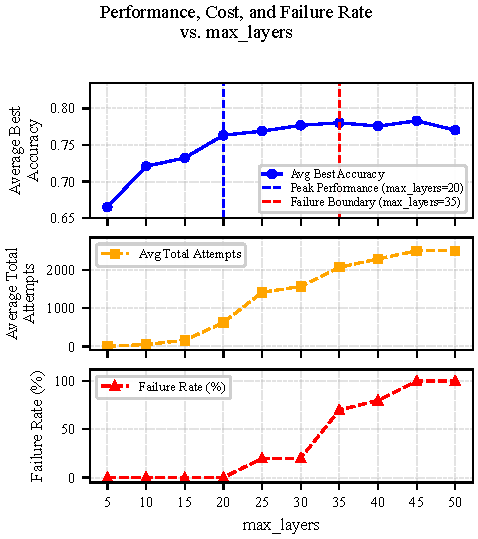
\includegraphics[width=\linewidth]{images/rebuttal_format/scaling_behavior_split.pdf}
\end{minipage}\hfill
\begin{minipage}[t]{0.48\linewidth}
\centering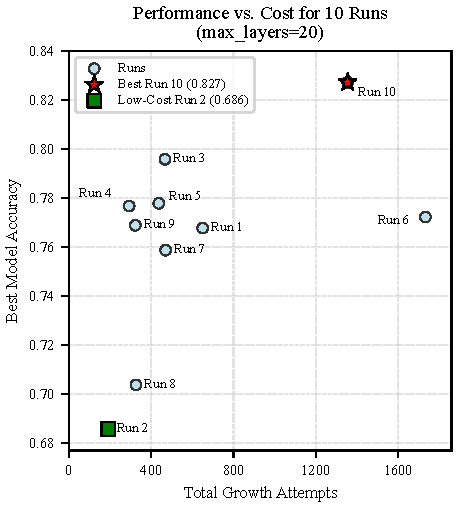
\includegraphics[width=\linewidth]{images/rebuttal_format/run_comparison_20.pdf}
\end{minipage}
\caption{Original LayerGrow study. Left: performance, cost and attempt-budget exhaustion versus the configured maximum depth. Right: variation among ten runs with a maximum of twenty layers. Configured depth differs from realized depth.}
\label{fig:scaling_behavior}
\end{figure}


\textit{\textbf{Positioning}: This appendix summarizes the \textbf{minimal configuration set} and \textbf{full statistical results} required to reproduce Experiment 1. For experimental objectives, core findings, and framework-level conclusions, please refer to Main Text \S~\ref{subsec:layergrow_validation}.}

\subsubsection{Dataset and Task}
\begin{table}[htbp]
    \centering
    \caption{Dataset and Task Configuration}
    \label{tab:dataset_config}
    \begin{tabular}{|p{3.5cm}|p{9cm}|}
        \hline
        \textbf{Item} & \textbf{Configuration} \\ \hline
        \textbf{Dataset} & Titanic Dataset. Only the training set is used for validation, stratified by \texttt{Survived} into 80\% training / 20\% testing. \\ \hline
        \textbf{Task Type} & Binary Classification. 
        \newline 
        \textit{Note:} This is a benchmark for structural exploration capability, \textbf{not} for generalization performance evaluation. It aims to reveal saturation and failure boundaries of search strategies in discrete space. \\ \hline
        \textbf{Evaluation Metric} & Test set accuracy (\texttt{best\_model\_accuracy}). \\ \hline
    \end{tabular}
\end{table}

\subsubsection{Method Pool Configuration (9 Scalar Operations)}
\begin{lstlisting}[style=plaincode]
# All methods have scalar input/output types, supporting type-safe routing
[
    "return_value",           # Identity mapping
    "return_two_values",      # Single input, dual output
    "add_values",             # Addition
    "calculate_difference",   # Subtraction
    "multiply_values",        # Multiplication
    "divide_values",          # Division (zero-protected)
    "increment",              # +1
    "decrement",              # -1
    "negate_value"            # Negation
]
\end{lstlisting}

\textit{\textbf{Design Principles}: Type consistency + Low-dimensional data flow + Determinism. Excluding semantic heterogeneity interference to focus on validating the navigation capability of the LayerGrow probe in pure structural combinatorial space.}

\subsubsection{Hyperparameter Grid}
\begin{table}[htbp]
    \centering
    \caption{Hyperparameter Settings}
    \label{tab:hyperparams}
    \small
    \renewcommand{\arraystretch}{1.15}
    \begin{tabularx}{\linewidth}{|>{\raggedright\arraybackslash}p{0.31\linewidth}|>{\raggedright\arraybackslash}X|}
        \hline
        \textbf{Parameter} & \textbf{Value/Description} \\ \hline
        \texttt{max\_layers} & \texttt{[5, 10, 15, 20, 25, 30, 35, 40, 45, 50]} \\ \hline
        \texttt{max\_attempts} (per layer) & 10 \\ \hline
        Rollback layers & 2 \\ \hline
        \texttt{decision\_threshold} & 0.0 \\ \hline
        \textbf{Max Total Attempts} & \textbf{2500} (Forced termination upon reaching limit is defined as ``failure'' and included in failure rate statistics) \\ \hline
        Independent Repetitions & 10 times/configuration \\ \hline
        Random Seed & Base 42, expanded per run: $\mathrm{seed}=42r+\mathrm{hash}(\texttt{max\_layers\_}L)\bmod 1000$ ($r\in[1,10]$) \\ \hline
    \end{tabularx}
\end{table}

\subsubsection{Full Statistical Results}
Table~\ref{tab:convergence_stats_appendix} reports detailed statistical metrics for each \texttt{max\_layers} configuration. The data corresponds to the trend curves in Fig.~\ref{fig:scaling_behavior}.

\begin{itemize}
    \item \textbf{Performance Saturation Point}: Mean best accuracy saturates at \texttt{max\_layers=20} ($0.763 \pm 0.041$, 0\% failure); for larger budgets it fluctuates only within statistical noise (0.769--0.783 at 25--50 layers) while the attempt-budget exhaustion rate climbs toward 100\%.
    \item \textbf{Attempt-budget exhaustion}: At configured maxima of 25 and 30 layers, 20\% of runs exhaust the 2,500-attempt budget; at maxima of 45 and 50, all runs do. Their mean realized depths are only 19.6 and 18.7 layers, respectively (Table~\ref{tab:convergence_stats_appendix}). These results locate a bottleneck of the tested growth strategy under a fixed attempt budget, rather than a failure to execute 45- or 50-layer graphs.
    \item \textbf{Path Dependence}: Even at the optimal configuration (20 layers), the standard deviation reaches 0.041, reflecting the sensitivity of discrete search to initial conditions. \item \textbf{Aggregation Rule}: All Avg Best Acc values are the mean, over the 10 independent runs, of the best model observed during each run---including runs terminated by the 2,500-attempt cap (failures)---consistent with the reporting convention in Main Text \S\ref{subsec:layergrow_validation}.
\end{itemize}

\begin{table}[htbp]
    \centering
    \resizebox{\linewidth}{!}{%
    \begin{tabular}{cccccc}
        \toprule
        \texttt{max\_layers} & Avg Best Acc & Std Dev & Avg Actual Layers & Avg Total Attempts & Failure Rate (\%) \\
        \midrule
        5  & 0.665 & 0.042 & 5.0  & 6.5    & 0.0  \\
        10 & 0.721 & 0.030 & 10.0 & 50.5   & 0.0  \\
        15 & 0.732 & 0.036 & 15.0 & 160.5  & 0.0  \\
        \textbf{20} & \textbf{0.763} & \textbf{0.041} & \textbf{20.0} & \textbf{624.5}  & \textbf{0.0}  \\
        25 & 0.769 & 0.028 & 22.9 & 1414.9 & 20.0 \\
        30 & 0.777 & 0.025 & 26.3 & 1567.4 & 20.0 \\
        35 & 0.780 & 0.022 & 21.7 & 2069.2 & 70.0 \\
        40 & 0.776 & 0.020 & 23.3 & 2289.7 & 80.0 \\
        45 & 0.783 & 0.024 & 19.6 & 2500.0 & 100.0 \\
        50 & 0.770 & 0.032 & 18.7 & 2500.0 & 100.0 \\
        \bottomrule
    \end{tabular}%
    }
    \caption{Statistical results under different maximum layer settings. Failure rate is defined as the proportion of runs where \texttt{total\_growth\_attempts=2500}. The bolded row indicates the optimal balance point between performance and efficiency.}
    \label{tab:convergence_stats_appendix}
\end{table}

\subsubsection{Supplementary Notes and Reproduction Guidelines}
\begin{itemize}
    \item \textbf{Path Dependence Analysis Data}: The scatter plot in the right panel of Fig.~\ref{fig:scaling_behavior} is generated from the per-run summary \path{experiments/LayerGrowTrainer_exp1/experiment_results_summary.csv} (shipped; columns \texttt{run}, \texttt{best\_model\_accuracy}, \texttt{total\_growth\_attempts}) by \texttt{generate\_experiment\_figures.py}; no separate plot-data CSV is maintained.
    \item \textbf{Complete Logs}: Candidate methods, rollback events and per-attempt accuracy are recorded for every run in \texttt{exp\_max\_layers\_\textless L\textgreater/run\_\textless r\textgreater/training\_log.json} (100 files, $\approx$216\,MB in total; keys \texttt{attempt\_history} and \texttt{rollback\_events}). They are regenerated by \texttt{main.py} and are not shipped, for size.
    \item \textbf{Reproduction Script}: All configurations and statistics are reproduced by:\\
    \path{experiments/LayerGrowTrainer_exp1/main.py}.
\end{itemize}

\subsection{Experiment 2 Configuration Summary (Knowledge Transfer Validation)}
\label{sec:appendix_exp2}


\begin{figure}[tb]
\centering
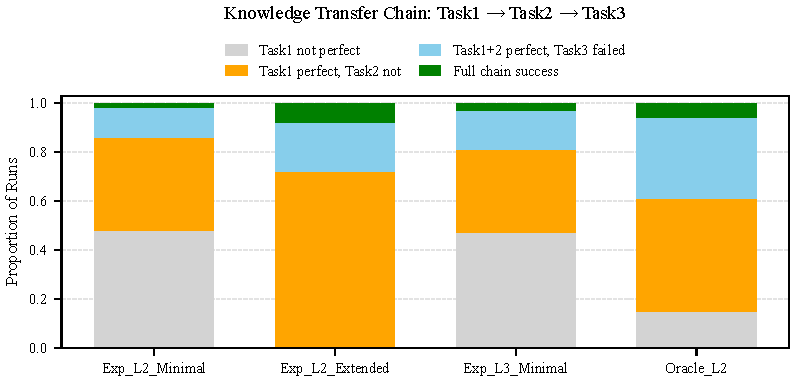
\includegraphics[width=0.82\linewidth]{images/rebuttal_format/exp3_knowledge_chain_from_logs.pdf}
\caption{Original three-task reuse experiment: the green fraction denotes runs completing the full knowledge-transfer chain.}
\label{fig:exp3_chain}
\end{figure}


\textit{\textbf{Positioning}: This appendix summarizes only the \textbf{minimal configuration set} required to reproduce Experiment 2. For experimental objectives, core findings, and framework-level conclusions, please refer to Main Text \S~\ref{subsec:graphevo_validation}.}

\subsubsection{Task and Evaluation Protocol}
\begin{table}[htbp]
    \centering
    \caption{Task and Evaluation Configuration}
    \label{tab:task_config}
    \small
    \renewcommand{\arraystretch}{1.15}
    \begin{tabularx}{\linewidth}{|>{\raggedright\arraybackslash}p{0.26\linewidth}|>{\raggedright\arraybackslash}X|}
        \hline
        \textbf{Item} & \textbf{Configuration} \\ \hline
        Task Chain & $f_1(x)=2(x+1)$\newline $\rightarrow f_2(x)=f_1(x)+3$\newline $\rightarrow f_3(x)=f_2(x)\times 0.5$ \\ \hline
        Data Type & Scalar \texttt{scalar}, resampled for each repetition (to eliminate data bias) \\ \hline
        Loss Function & MSE (Focuses on structural transfer validation, not numerical fitting upper bounds) \\ \hline
        Success Criterion & The reported Success Rate counts runs with Task~3 accuracy $> 0.95$; the stricter ``Complete Transfer Chain'' criterion (Tasks 1/2 $\ge 0.999$ \emph{and} Task~3 $> 0.95$) applies only to the breakdown in Fig.~\ref{fig:exp3_chain} \\ \hline
        Evaluation Metrics & Task 3 Mean Accuracy $\pm$ Std Dev, Success Rate (Successful Runs / 100) \\ \hline
    \end{tabularx}
\end{table}

\subsubsection{Method Pool Configuration (Three Variants, all operating on \texttt{scalar})}
\begin{lstlisting}[style=plaincode]
# Minimal (5 atomic operations)
[
    "increment",        # x -> x+1
    "multiply_by_2",    # x -> 2x
    "add_3",            # x -> x+3
    "multiply_by_05",   # x -> 0.5x
    "identity"          # x -> x
]

# Extended (Minimal + 1 item)
[...above 5 items..., "add_2"]  # x -> x+2

# Oracle (Static Injection): Minimal pool + f1_direct (6 items)
[
    "increment", "f1_direct",   # x -> x+1  |  x -> 2(x+1)
    "multiply_by_2", "add_3", "multiply_by_05", "identity"
]
\end{lstlisting}

\textit{\textbf{Design Principle}: All methods have input/output types of \texttt{scalar}, excluding type-matching interference to focus on validating structural composition capabilities.}

\subsubsection{Hyperparameters and Control Variables}
\begin{table}[htbp]
    \centering
    \caption{Hyperparameters and Control Variables}
    \label{tab:hyperparams_exp2}
    \resizebox{\linewidth}{!}{
    \begin{tabular}{|l|l|}
        \hline
        \textbf{Parameter} & \textbf{Value/Description} \\ \hline
        \texttt{max\_init\_layers} (Tasks 1/2) & 2 layers / 3 layers (two comparison groups) \\ \hline
        Method Pool Evolution & Enabled (\texttt{Exp}) / Disabled (\texttt{Ctrl}) / Static Injection (\texttt{Oracle}) \\ \hline
        Independent Repetitions & 100 times/configuration \\ \hline
        Random Seed Strategy & \texttt{42 + rep\_id} (\texttt{rep\_id} $\in [0, 99]$) \\ \hline
        Data Sampling & Regenerated for each repetition to avoid data bias \\ \hline
        Early Stopping Threshold & Task-level accuracy $\ge 0.999$ considered ``Perfect Mastery'' \\ \hline
    \end{tabular}
    }
\end{table}

\subsubsection{Supplementary Notes}
\begin{itemize}
    \item \textbf{Chain Analysis Definition}: ``Complete Knowledge Transfer Chain'' = Task 1 Perfect (Acc $\ge 0.999$) $\land$ Task 2 Perfect (Acc $\ge 0.999$) $\land$ Task 3 Success (Acc $> 0.95$), used to isolate structured transfer paths.
    \item \textbf{Accuracy Calculation Logic}: Based on \textit{Relative Error Threshold}. A sample is considered correct if $\frac{|\hat{y} - y|}{|y| + 10^{-8}} < 0.01$. Task accuracy is the proportion of correct samples in the dataset.
    \item \textbf{Method Pool Evolution Data}: The change in the total number of methods at each stage is computed from \texttt{exp3\_results/\textless config\textgreater/rep\textless k\textgreater/metadata.json} by \texttt{plot\_method\_pool\_evolution.py}; the rendered figure is shipped as \path{GraphEvo_exp3/method_pool_three_stage_evolution.png}.
    \item \textbf{Complete Statistics}: Accuracy for Tasks 1/2/3, method-pool snapshots and evolution trajectories are stored per run under \texttt{exp3\_results/\textless config\textgreater/rep\textless k\textgreater/} (100 repetitions per configuration, $\approx$10\,MB in total). They are regenerated by \texttt{exp3\_main.py} and are not shipped; the configuration-level summary backing Table~\ref{tab:exp3_results} is shipped as \path{exp3_results/summary_table.csv}.
\end{itemize}

Table~\ref{tab:exp3_results} reports the end-to-end performance of Task 3 under various configurations (100 repetitions). Figure~\ref{fig:exp3_chain} further decomposes the success paths of the knowledge transfer chain.

\begin{table}[htbp]
    \centering
    \caption{Performance comparison for Task 3 in Experiment 3. Evolution column: \checkmark = Method pool evolution enabled, \texttimes = Disabled, --- = Static injection baseline.}
    \label{tab:exp3_results}
    \resizebox{\linewidth}{!}{
    \begin{tabular}{llclcc}
        \toprule
        Group & Evolution & Max Layers & Method Pool & Avg Acc $\pm$ Std & Success Rate (\%) \\
        \midrule
        Ctrl\_L2\_Minimal & \texttimes & 2 & Minimal & $0.0006 \pm 0.0021$ & 0 \\
        Ctrl\_L2\_Extended & \texttimes & 2 & Extended & $0.0003 \pm 0.0012$ & 0 \\
        Ctrl\_L3\_Minimal & \texttimes & 3 & Minimal & $0.0007 \pm 0.0022$ & 0 \\
        \textbf{Exp\_L2\_Minimal} & \checkmark & 2 & Minimal & \textbf{$0.1308 \pm 0.3360$} & \textbf{13} \\
        Exp\_L2\_Extended & \checkmark & 2 & Extended & $0.1312 \pm 0.3359$ & 13 \\
        Exp\_L3\_Minimal & \checkmark & 3 & Minimal & $0.0908 \pm 0.2859$ & 9 \\
        Oracle\_L2 & --- & 2 & Oracle & $0.1206 \pm 0.3247$ & 12 \\
        \bottomrule
    \end{tabular}
    }
\end{table}

\subsection{Experiment 3 Configuration and Supplementary Data (Topology-Aware Task Parallelism)}
\label{sec:appendix_exp3}

\subsubsection{Experimental Motivation and Core Findings}
To validate the \textbf{structural-level parallel schedulability} of GDFG during the inference phase, we evaluated the scalability of a topology-aware dynamic task parallelism mechanism in a multi-core CPU environment. This experiment aims to address two framework-level questions:
\begin{enumerate}
    \item Does the explicit dependency metadata in GDFG support \textbf{lock-free or low-conflict parallel scheduling}?
    \item How do the topological characteristics of the graph constrain the \textbf{parallel efficiency boundaries} of the representation space on real hardware?
\end{enumerate}

Experimental results show that under simulated I/O or non-blocking loads, shallow wide graphs achieved a mean speedup of $10.25\times$ on 16 cores, i.e.\ $64\%$ of the ideal linear bound, with efficiency still near $90\%$ at 8 cores. This confirms that the DAG structure of GDFG naturally supports fine-grained task parallelism. Further analysis indicates that parallel efficiency is strongly positively correlated with the graph's \textbf{Average Width} (Pearson $r \approx 0.99$ across the 30 graphs at 16 cores), rather than its total node count ($r \approx -0.16$) or depth ($r \approx -0.41$), suggesting that ``wide and shallow'' topological structures are more conducive to multi-core utilization. These measurements use simulated I/O or non-blocking operators. Type-compatible edges validate data interfaces; shared-state conflicts are handled separately by the execution contract in Appendix~\ref{app:revision_effects}.

This experiment confirms that the AdaptoFlux representation space possesses \textbf{native parallel potential}. Its performance is primarily constrained by the graph's average width and the scheduling granularity of the backend execution model. This provides clear guidelines for subsequent optimization: structurally, evolution should encourage the generation of high-concurrency, wide-shallow topologies to maximize the utilization of modern multi-core hardware; engineering-wise, migrating to GIL-free backends (such as C++ extensions or process pools) can further unlock the theoretical parallel upper bound. Detailed experimental configurations, structural metric analyses, and flame graph evidence are provided in the following subsections.

\begin{figure}[htbp]
    \centering
    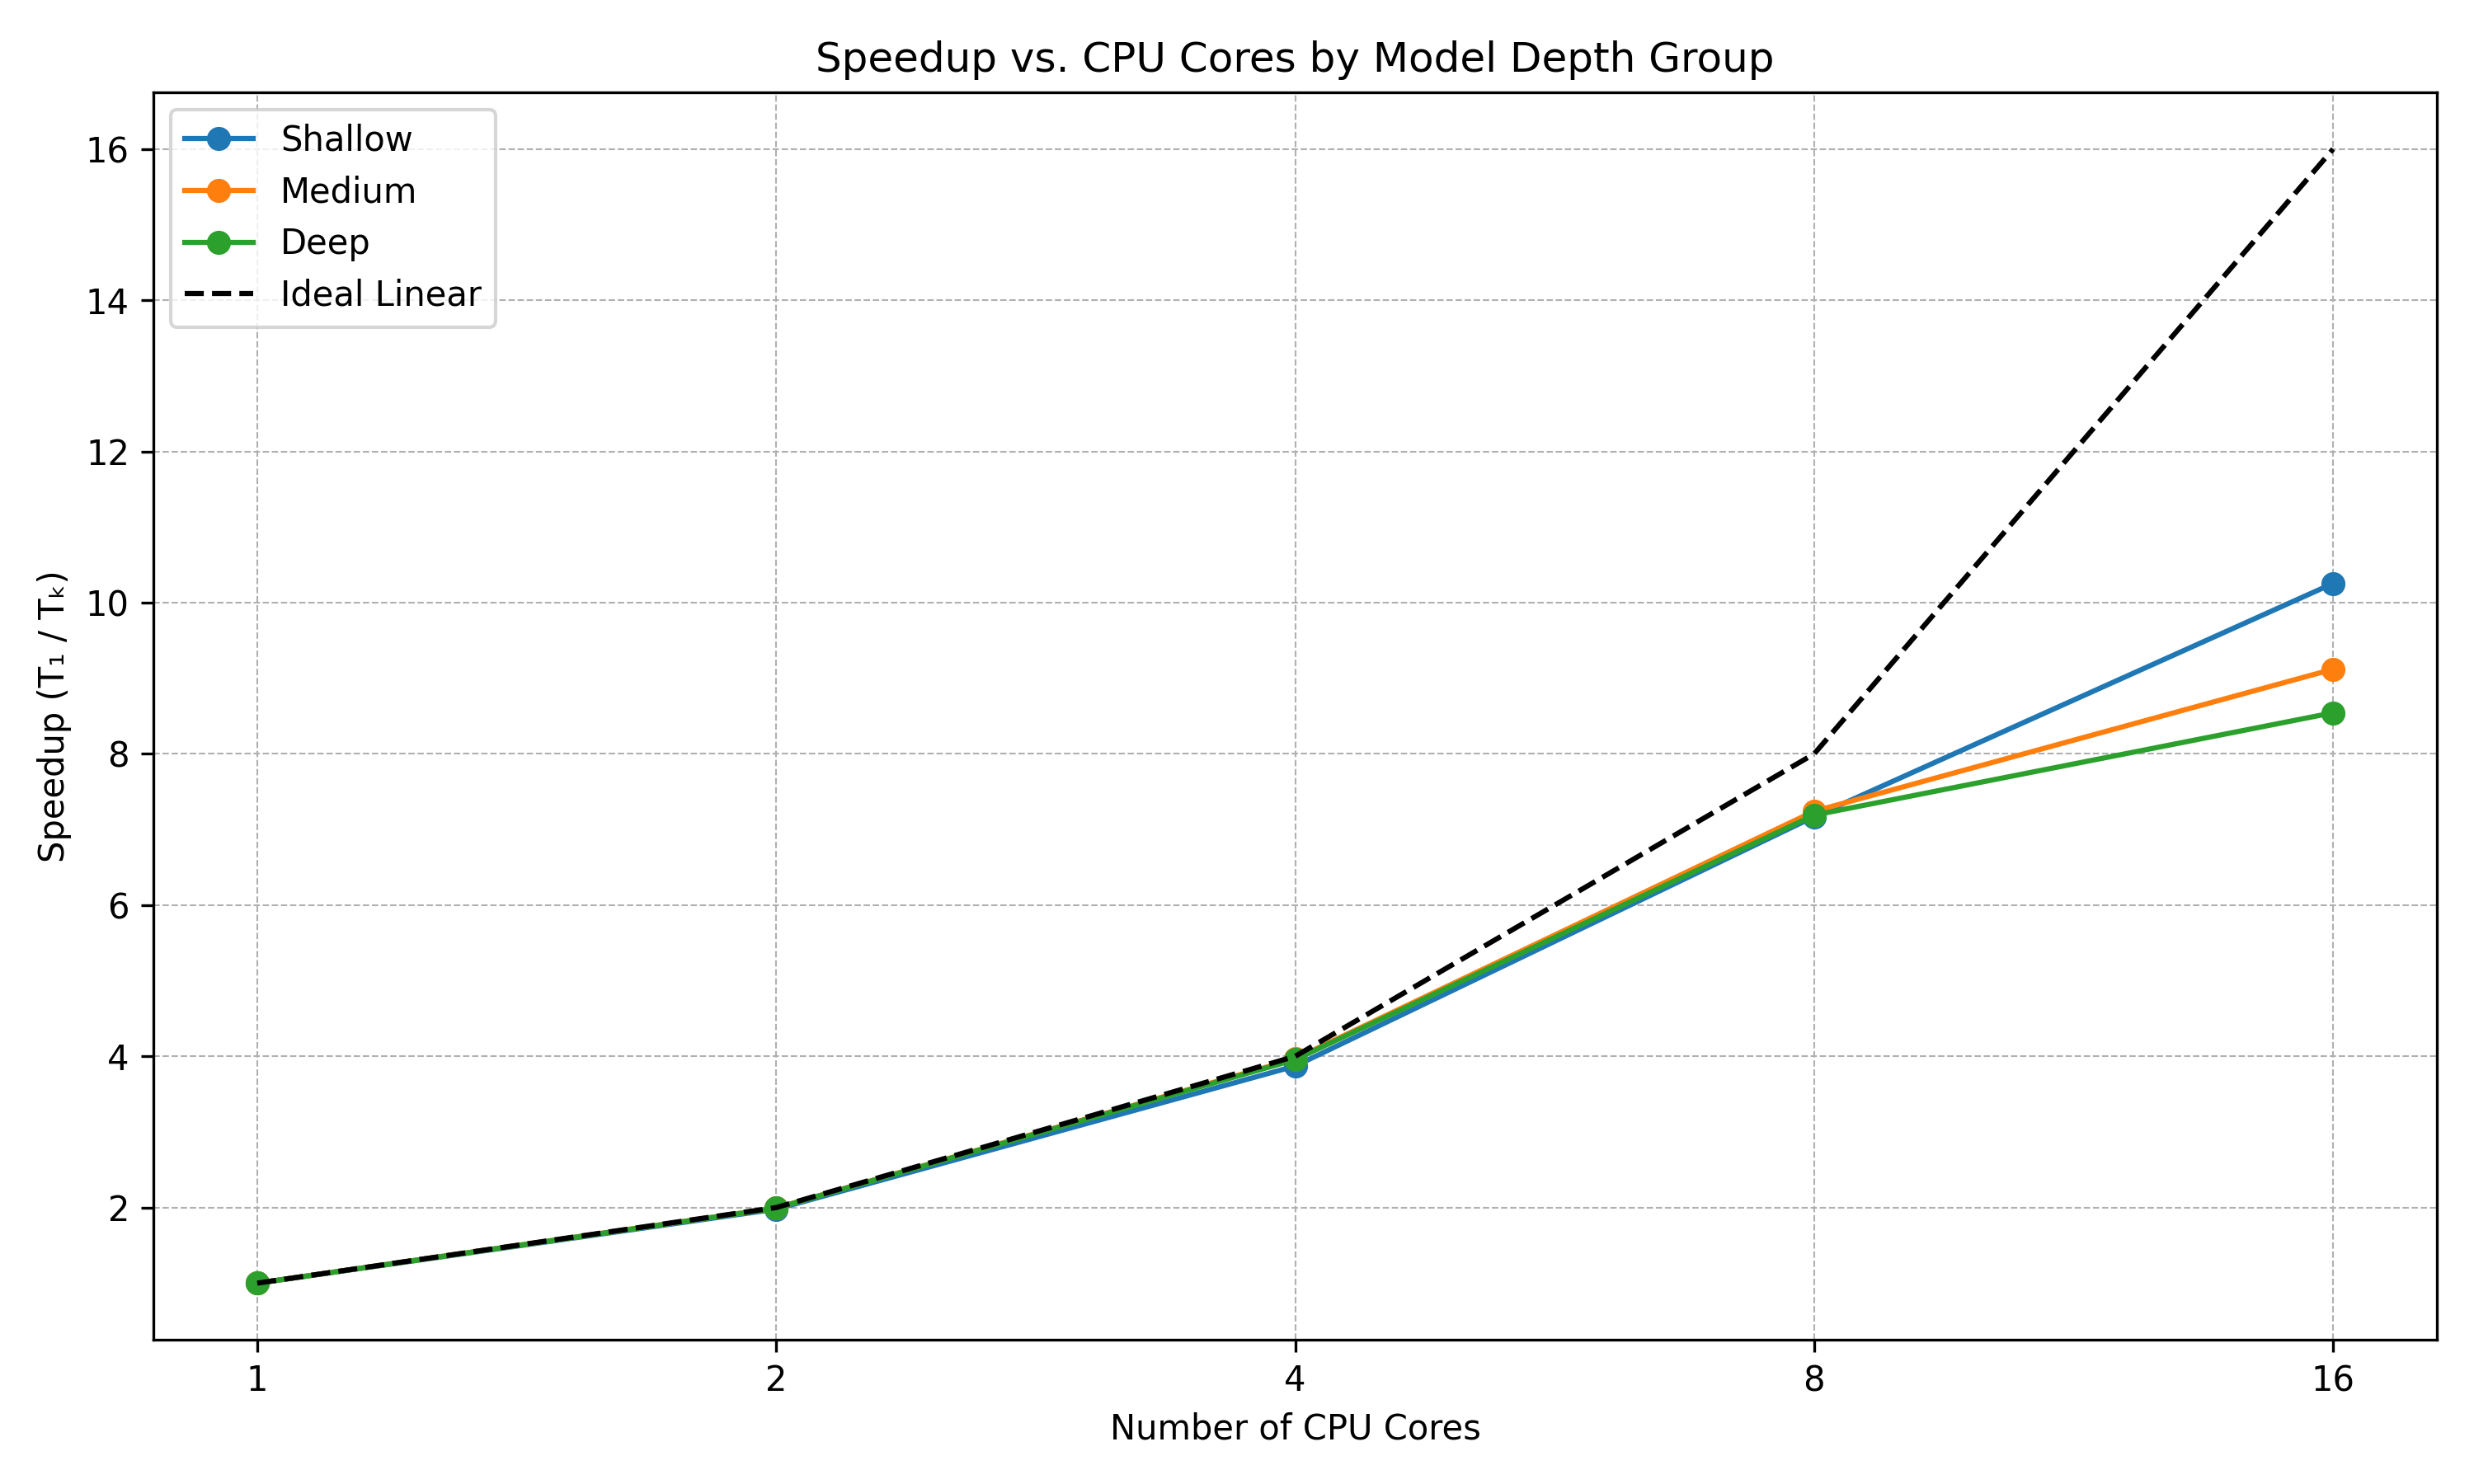
\includegraphics[width=0.85\linewidth]{images/exp_2/task_parallel_speedup_cpu_nogil.png}
    \caption{Average speedup under GIL-releasable scenarios. Different depth model groups under simulated non-blocking loads. The dashed line represents ideal linear speedup. Shallow wide graphs achieve a \textbf{10.25$\times$} speedup on 16 cores.}
    \label{fig:task_parallel_speedup_comparison}
\end{figure}

\subsubsection{Experimental Environment and Core Configuration}

\paragraph{Hardware and Software Environment}
\begin{itemize}
    \item \textbf{Executor}: Dynamic task scheduler implemented based on Python \texttt{concurrent.futures.ThreadPoolExecutor}.
    \item \textbf{Hardware Platform}: Multi-core CPU environment on the same server, with other process interference isolated.
    \item \textbf{Parallel Granularity}: Number of threads $K \in \{1, 2, 4, 8, 16\}$, simulating concurrency capabilities of different core counts.
    \item \textbf{Load Simulation Modes}:
    \begin{itemize}
        \item \textbf{GIL-Constrained Scenario (No-Sleep)}: Nodes execute pure Python lightweight computations, constrained by the Global Interpreter Lock, preventing true parallelism.
        \item \textbf{GIL-Releasable Scenario (Sleep)}: every method in the pool calls \texttt{time.sleep(0.001)} inside its own implementation before returning, simulating a 1\,ms I/O wait or C-extension call so that threads release the GIL and achieve CPU-level parallelism.
    \end{itemize}
\end{itemize}

\paragraph{Control Variables}
\begin{itemize}
    \item \textbf{Fixed Variables}:
    \begin{itemize}
        \item Dataset: Titanic (Titanic Survival Prediction).
        \item Input Batch Size: Kept consistent.
        \item Method Pool Configuration: Uses the simplified method pool from Experiment 1 (see Appendix~\ref{sec:appendix_exp1}).
        \item Random Seed: 42.
    \end{itemize}
    \item \textbf{Variable Variables}:
    \begin{itemize}
        \item Number of computation threads $K$.
        \item Model topology structures (different evolution results from Experiment 1 training logs, see Appendix~\ref{sec:appendix_exp1}).
    \end{itemize}
\end{itemize}

\subsubsection{Experimental Subjects: Detailed List of 30 DAG Models}

In the main text, models are divided into shallow, medium, and deep groups based on depth. The table below lists the detailed source information for all 30 models participating in the experiment, including maximum allowed layers (\texttt{max\_layers}), run sequence (\texttt{run}), model type (\texttt{model\_type}), and actual constructed layers.

\begin{table}[htbp]
    \centering
    \caption{Source and Structural Information of the 30 Models Used in Experiment 3}
    \label{tab:exp3_models_list}
    \resizebox{\linewidth}{!}{%
    \begin{tabular}{cccccc}
        \toprule
        \textbf{ID} & \texttt{max\_layers} & \texttt{run} & \texttt{model\_type} & \textbf{Actual Layers} & \textbf{Group} \\
        \midrule
        1 & 5 & 1 & final & 5 & Shallow \\
        2 & 5 & 5 & final & 5 & Shallow \\
        3 & 5 & 6 & final & 5 & Shallow \\
        4 & 10 & 1 & best & 9 & Shallow \\
        5 & 10 & 2 & best & 2 & Shallow \\
        6 & 10 & 4 & best & 8 & Shallow \\
        7 & 10 & 5 & best & 5 & Shallow \\
        8 & 10 & 8 & best & 6 & Shallow \\
        9 & 5 & 7 & final & 5 & Shallow \\
        10 & 5 & 8 & final & 5 & Shallow \\
        11 & 15 & 1 & best & 12 & Medium \\
        12 & 15 & 4 & final & 15 & Medium \\
        13 & 15 & 8 & best & 11 & Medium \\
        14 & 15 & 9 & final & 15 & Medium \\
        15 & 20 & 1 & final & 20 & Medium \\
        16 & 20 & 3 & best & 9 & Shallow \\
        17 & 20 & 4 & final & 20 & Medium \\
        18 & 20 & 5 & final & 20 & Medium \\
        19 & 20 & 7 & best & 17 & Medium \\
        20 & 20 & 9 & final & 20 & Medium \\
        21 & 25 & 6 & final & 25 & Deep \\
        22 & 25 & 7 & final & 25 & Deep \\
        23 & 25 & 10 & best & 23 & Deep \\
        24 & 30 & 2 & best & 22 & Deep \\
        25 & 30 & 3 & final & 30 & Deep \\
        26 & 30 & 7 & best & 15 & Medium \\
        27 & 30 & 8 & final & 30 & Deep \\
        28 & 35 & 2 & best & 27 & Deep \\
        29 & 35 & 5 & final & 35 & Deep \\
        30 & 30 & 1 & best & 11 & Medium \\
        \bottomrule
    \end{tabular}%
    }
\end{table}

\textit{\textbf{Note}: Models are classified by actual layer count: Shallow (1--10 layers), Medium (11--20 layers), Deep (21--35 layers). Some models have actual layers less than \texttt{max\_layers} due to early termination during evolution.}

\subsubsection{Supplementary Analysis: Relationship Between Node Scale and Parallel Efficiency}

The main text states that ``total node count is not the core factor determining parallel efficiency.'' To verify this conclusion, we regrouped the 30 models by \textbf{total node count} and statistically analyzed their performance under different core counts.

\paragraph{Performance Statistics Grouped by Node Scale}

\begin{table}[htbp]
    \centering
    \caption{Average Performance of Models with Different Node Scales on Multi-Core CPUs (No-GIL Valid Data Only)}
    \label{tab:exp3_node_scale_perf}
    \resizebox{\linewidth}{!}{%
    \begin{tabular}{lcccc}
        \toprule
        \textbf{Node Scale Range} & \textbf{CPU Cores} & \textbf{Avg Speedup ($S_K$)} & \textbf{Avg Efficiency ($E_K$)} & \textbf{Efficiency Std Dev} \\
        \midrule
        \textbf{Small ($\le$93)} & 1 & $1.00\times$ & $100.0\%$ & --- \\
        (10 models) & 4 & $3.86\times$ & $96.6\%$ & $2.7\%$ \\
         & 8 & $7.13\times$ & $89.1\%$ & $6.1\%$ \\
         & 16 & $10.19\times$ & $63.7\%$ & $8.1\%$ \\
        \midrule
        \textbf{Medium (94--190)} & 1 & $1.00\times$ & $100.0\%$ & --- \\
        (10 models) & 4 & $3.96\times$ & $99.0\%$ & $0.7\%$ \\
         & 8 & $7.11\times$ & $88.9\%$ & $8.7\%$ \\
         & 16 & $8.92\times$ & $55.8\%$ & $11.5\%$ \\
        \midrule
        \textbf{Large ($\ge$191)} & 1 & $1.00\times$ & $100.0\%$ & --- \\
        (10 models) & 4 & $3.97\times$ & $99.1\%$ & $0.6\%$ \\
         & 8 & $7.36\times$ & $92.0\%$ & $5.4\%$ \\
         & 16 & $9.03\times$ & $56.5\%$ & $8.3\%$ \\
        \bottomrule
    \end{tabular}%
    }
\end{table}

\textbf{Analysis}: \\
As seen in Table~\ref{tab:exp3_node_scale_perf}, although the large-scale group has a slightly higher absolute speedup under 16 cores ($9.03\times$ vs $8.92\times$), its efficiency fluctuation (standard deviation) is not significantly better than the small/medium groups. More importantly, the small-scale group achieved the highest average speedup ($10.19\times$) under 16 cores, directly refuting the intuitive assumption that ``larger models are harder to parallelize.''

\paragraph{Scatter Distribution of Node Count vs. Speedup}

\begin{figure}[htbp]
    \centering
    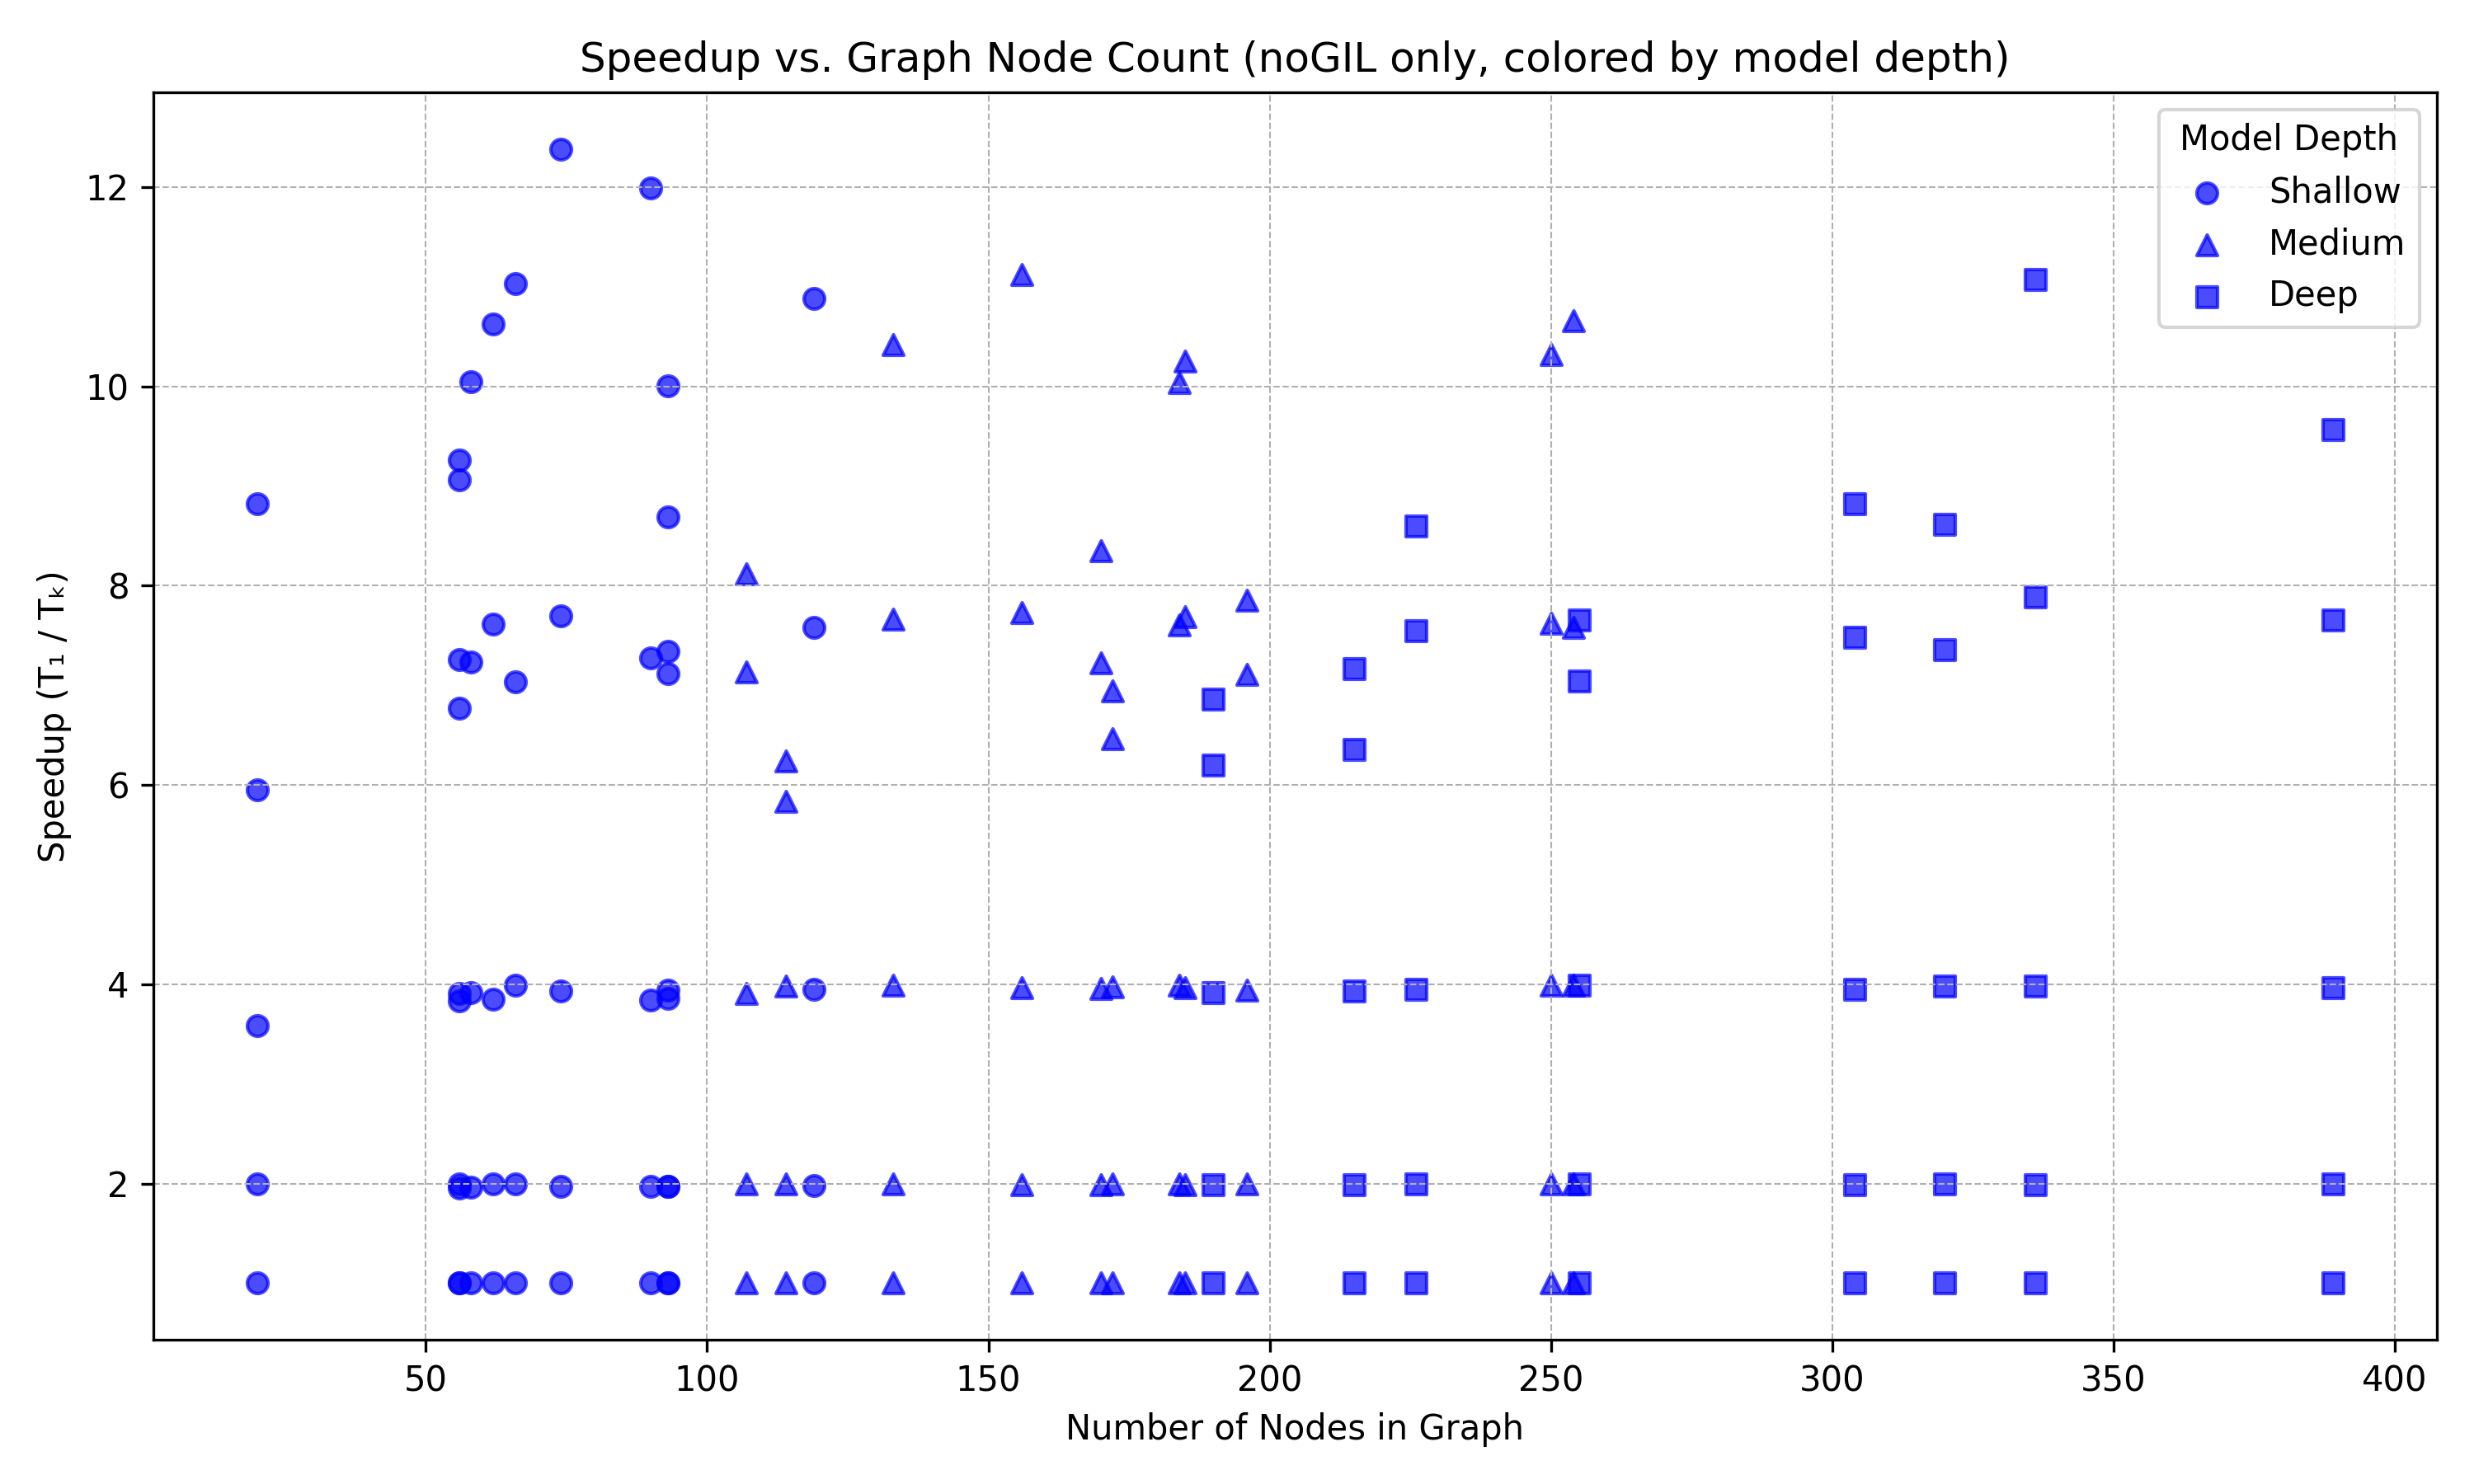
\includegraphics[width=0.8\linewidth]{images/speedup_vs_node_count.png}
    \caption{Scatter plot of node count vs. speedup (No-GIL data only). X-axis: Total nodes in graph; Y-axis: Speedup $S_K = T_1 / T_K$. Different marker shapes represent model depth (Circle: Shallow, Triangle: Medium, Square: Deep).}
    \label{fig:speedup_vs_nodes}
\end{figure}

\textbf{Observation}: \\
Fig.~\ref{fig:speedup_vs_nodes} shows that the vertical distribution of speedup has no obvious monotonic correlation with the horizontal axis of node count. Whether with dozens of small nodes or hundreds of large nodes, speedups are distributed within the $8\times$--$10\times$ range. This further confirms that \textbf{the total node count of the graph structure is not the core factor determining pipeline parallel efficiency}.

\subsubsection{Supplementary Analysis: Impact of Structural Heterogeneity Metrics}

Besides depth and width, local connectivity characteristics of the graph (such as branching rate, out-degree) may also affect scheduling complexity. We extracted the following structural metrics for analysis:
\begin{itemize}
    \item \textbf{Branching Rate}: Proportion of nodes with out-degree $\ge 2$.
    \item \textbf{Average Out-Degree}: Average number of output edges for all nodes in the graph.
\end{itemize}

\begin{figure}[htbp]
    \centering
    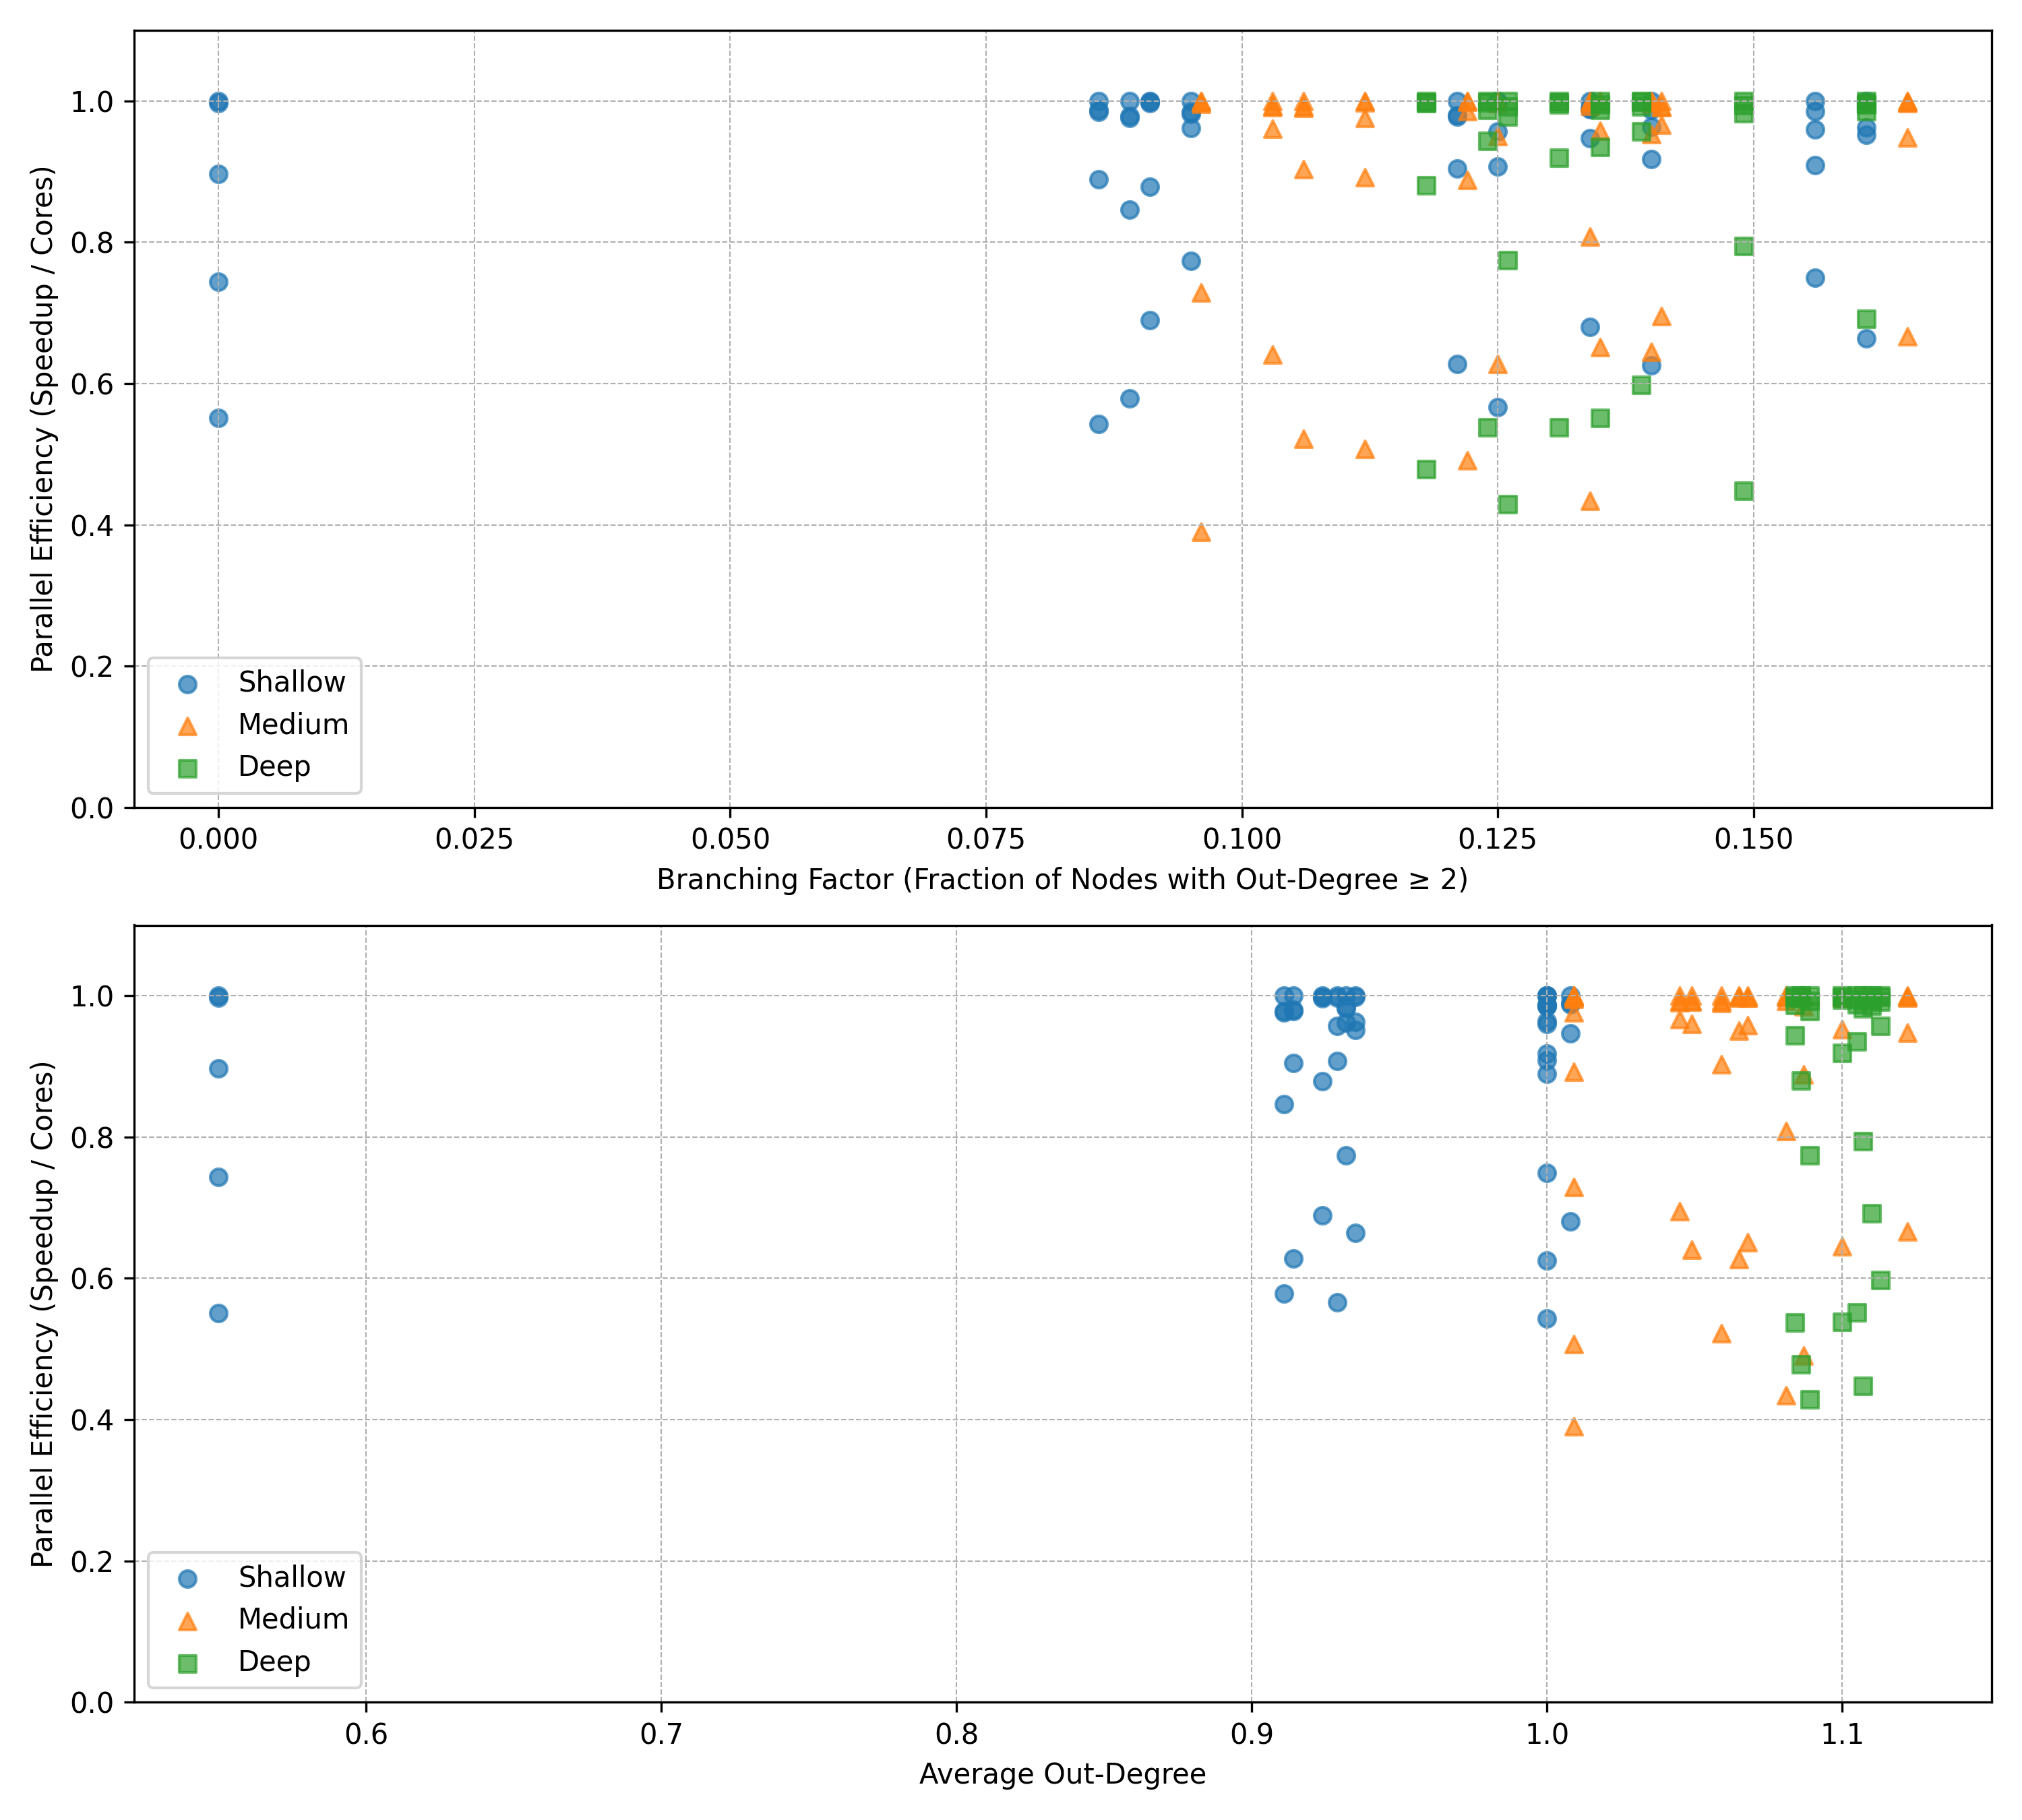
\includegraphics[width=0.8\linewidth]{images/exp_2/efficiency_vs_branching_and_outdegree.png}
    \caption{Scatter plots of structural heterogeneity metrics vs. speedup (No-GIL data only). (a) Branching Rate vs. Speedup; (b) Average Out-Degree vs. Speedup.}
    \label{fig:heterogeneity_speedup}
\end{figure}

\textbf{Analysis}:
\begin{itemize}
    \item \textbf{No Significant Correlation}: Fig.~\ref{fig:heterogeneity_speedup} shows that high branching rate or high average out-degree did not lead to a systematic decrease in speedup.
    \item \textbf{Coupling of Depth and Heterogeneity}: Notably, deep models (square markers) tend to cluster in regions of high branching rate and high out-degree. This indicates that as evolution layers deepen, the graph structure naturally tends towards more complex connection patterns. However, this increase in complexity did not impose a significant burden on AdaptoFlux's topology-aware scheduling, demonstrating that the in-degree-based dynamic scheduling algorithm has good robustness to local heterogeneity.
\end{itemize}

\subsubsection{Micro-Performance Profiling: Flame Graph Evidence}

To deeply understand the impact mechanism of GIL on task parallelism, we selected three representative models: Shallow (6 layers), Medium (15 layers), and Deep (25 layers), and collected execution flame graphs for both GIL-constrained and GIL-releasable scenarios.

\paragraph{Flame Graph Comparison Overview}

% 原图宽度均为 1200 像素，未包含分辨率元数据。按原始坐标将左右各 600 像素
% 分别放大到正文宽度，完整保留截图内容，避免缩小整张截图后函数名无法辨认。
% 后五页使用同一图号的延续说明，不重置 figure 计数器，避免重复超链接目标。
\newcommand{\atfFlameGraphHalves}[1]{%
    {\small\textit{Left half of the recorded display}}\par\smallskip
    \includegraphics[width=\linewidth,trim={0 0 600bp 0},clip]{#1}\par\medskip
    {\small\textit{Right half of the recorded display}}\par\smallskip
    \includegraphics[width=\linewidth,trim={600bp 0 0 0},clip]{#1}\par
}

\begin{figure}[p]
    \centering
    {\small\textbf{(a)} Shallow model (6 layers), pure Python computation}\par\medskip
    \atfFlameGraphHalves{images/exp_2/flamegraph/model_8_nosleep.png}
    \caption{Flame graph comparison for representative models. Each original screenshot is enlarged as two horizontal halves, preserving its complete display. Panels (a), (c) and (e) use GIL-constrained pure Python computation; panels (b), (d) and (f) use GIL-releasable computation with injected \texttt{time.sleep}. The six panels continue on the following pages.}
    \label{fig:flamegraphs}
\end{figure}

\begin{figure}[p]
    \centering
    {\small\textbf{(b)} Shallow model (6 layers), injected \texttt{time.sleep}}\par\medskip
    \atfFlameGraphHalves{images/exp_2/flamegraph/model_8_sleep.png}
    \par\medskip{\small Figure~\ref{fig:flamegraphs} (continued): shallow model, GIL-releasable scenario.}
\end{figure}

\begin{figure}[p]
    \centering
    {\small\textbf{(c)} Medium model (15 layers), pure Python computation}\par\medskip
    \atfFlameGraphHalves{images/exp_2/flamegraph/model_14_nosleep.png}
    \par\medskip{\small Figure~\ref{fig:flamegraphs} (continued): medium model, GIL-constrained scenario.}
\end{figure}

\begin{figure}[p]
    \centering
    {\small\textbf{(d)} Medium model (15 layers), injected \texttt{time.sleep}}\par\medskip
    \atfFlameGraphHalves{images/exp_2/flamegraph/model_14_sleep.png}
    \par\medskip{\small Figure~\ref{fig:flamegraphs} (continued): medium model, GIL-releasable scenario.}
\end{figure}

\begin{figure}[p]
    \centering
    {\small\textbf{(e)} Deep model (25 layers), pure Python computation}\par\medskip
    \atfFlameGraphHalves{images/exp_2/flamegraph/model_21_nosleep.png}
    \par\medskip{\small Figure~\ref{fig:flamegraphs} (continued): deep model, GIL-constrained scenario.}
\end{figure}

\begin{figure}[p]
    \centering
    {\small\textbf{(f)} Deep model (25 layers), injected \texttt{time.sleep}}\par\medskip
    \atfFlameGraphHalves{images/exp_2/flamegraph/model_21_sleep.png}
    \par\medskip{\small Figure~\ref{fig:flamegraphs} (continued): deep model, GIL-releasable scenario.}
\end{figure}

\textbf{Micro-Profiling Conclusion}:
\begin{itemize}
    \item \textbf{Panels (a), (c), (e): GIL-Constrained}: The \texttt{wrapped} node (computation logic) is extremely narrow in the flame graph, almost drowned out by scheduler overhead (dependency tracking, lock contention, logging). This indicates that multi-threading cannot execute computations concurrently, only incurring additional synchronization costs.
    \item \textbf{Panels (b), (d), (f): GIL-Releasable}: The width of the \texttt{wrapped} function increases significantly, showing overlapping execution across different threads. This confirms that when node computation can release the GIL, AdaptoFlux's topology-aware scheduling mechanism effectively exposes node-level parallel potential, and the coarse-grained tasks introduced by \texttt{time.sleep} further reduce the relative overhead of context switching.
\end{itemize}

\textit{\textbf{Note}: In the flame graphs, the \texttt{wrapped} function may appear as \texttt{wrap..} or nested under \texttt{process\_node} due to sampling rate or namespace folding; its true meaning is the node computation proxy function.}

\paragraph{Detailed Interpretation}

\begin{enumerate}
    \item \textbf{GIL-Constrained Scenario (Panels (a), (c), (e))}:
    \begin{itemize}
        \item \textbf{Phenomenon}: The \texttt{wrapped} node (i.e., user-defined computation logic) is extremely narrow in the flame graph, almost invisible.
        \item \textbf{Dominant Overhead}: CPU time is mainly consumed by internal scheduler logic, including:
        \begin{itemize}
            \item Dependency checking and in-degree updating (\texttt{decrement\_indegree}).
            \item Thread lock contention (\texttt{threading.Lock.acquire}).
            \item Logging and status synchronization.
        \end{itemize}
        \item \textbf{Conclusion}: In pure Python computation, multi-threading not only fails to parallelize computation but also leads to ``negative acceleration'' due to frequent context switching and lock contention.
    \end{itemize}
    
    \item \textbf{GIL-Releasable Scenario (Panels (b), (d), (f))}:
    \begin{itemize}
        \item \textbf{Phenomenon}: The width of the \texttt{wrapped} function increases significantly, occupying the main part of the flame graph.
        \item \textbf{Parallel Exposure}: Multiple \texttt{wrapped} blocks overlap on the timeline, indicating that different threads are executing different node computations simultaneously.
        \item \textbf{Reduced Scheduler Overhead Ratio}: Although scheduling logic still exists, its relative proportion shrinks significantly because the coarse-grained tasks simulated by \texttt{time.sleep} make computation/wait time much larger than scheduling overhead.
        \item \textbf{Conclusion}: Once node computation can release the GIL (e.g., I/O, C extensions, or explicit sleep), AdaptoFlux's topology-aware scheduling mechanism efficiently distributes tasks to idle cores, fully exposing parallel potential.
    \end{itemize}
\end{enumerate}

\subsubsection{Scheduling Algorithm Pseudocode}

AdaptoFlux employs a topological sorting-based dynamic task scheduling algorithm, as shown below:

\begin{lstlisting}[language=Python, caption={Topological Dynamic Schedule}]
def topological_dynamic_schedule(graph, thread_pool):
    # 1. Initialization: Calculate remaining in-degree for each node
    remaining_in_degree = {node: len(node.predecessors) for node in graph.nodes}
    
    # 2. Ready Queue: Find all nodes with initial in-degree 0 (excluding root)
    ready_queue = [node for node in graph.nodes if remaining_in_degree[node] == 0 and node != root]
    
    futures = []
    
    while ready_queue or futures:
        # 3. Submit Tasks: Take nodes from ready queue and submit to thread pool
        while ready_queue:
            node = ready_queue.pop(0)
            future = thread_pool.submit(execute_node, node)
            future.add_done_callback(lambda f, n=node: on_node_complete(n, f))
            futures.append(future)
            
        # 4. Wait and Callback Processing
        for future in as_completed(futures):
            node = future_to_node_map[future]
            futures.remove(future)
            
            # 5. Update Successor Node Status
            for successor in node.successors:
                remaining_in_degree[successor] -= 1
                if remaining_in_degree[successor] == 0:
                    ready_queue.append(successor)
                    
def execute_node(node):
    # Execute the method bound to the node
    result = node.method(*node.inputs)
    return result
\end{lstlisting}

% ==============================================================================
% APPENDIX C.4: Minimal Stateful Attractor (automatic stateful synthesis)
% ==============================================================================

\subsection{Experiment 4 Configuration and Full Statistical Results (Minimal Stateful Attractor)}
\label{sec:appendix_exp4}


\begin{figure}[tb]
\centering
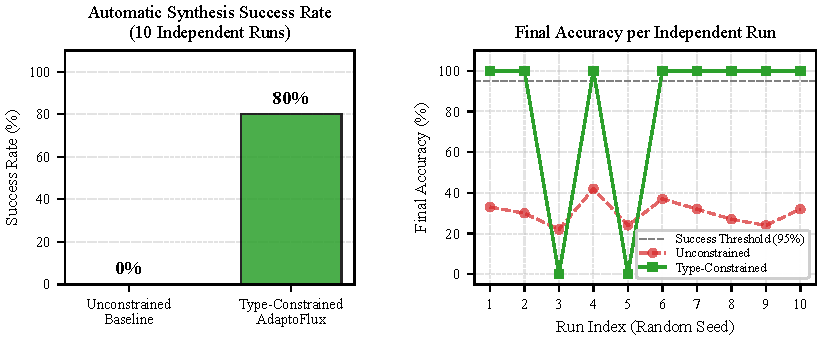
\includegraphics[width=0.92\linewidth]{images/rebuttal_format/stateful_synthesis_comparison.pdf}
\caption{Original ten-seed stateful-synthesis experiment: success rates of 0/10 and 8/10, with per-run accuracy under its randomized evaluation protocol. The exhaustive thirty-seed comparison appears separately in Appendix~\ref{app:revision_types}.}
\label{fig:stateful_synthesis}
\end{figure}


\paragraph{Historical protocol.}
This section preserves the original ten-seed experiment and its randomized episode evaluation. The new three-condition, thirty-seed comparison in Appendix~\ref{app:revision_types} evaluates all twenty unequal initial position--target pairs. These are separate protocols, and their run counts are reported separately.


\textit{\textbf{Positioning}: This appendix summarizes only the \textbf{minimal configuration set} required to reproduce the automatic stateful synthesis experiment of Main Text \S~\ref{subsec:stateful_synthesis}. For the experimental objective and the framework-level interpretation, please refer to that section.}

\subsubsection{Task and Evaluation Protocol}
\begin{table}[htbp]
    \centering
    \caption{Minimal Stateful Attractor: task and evaluation configuration}
    \label{tab:stateful_task_config}
    \small
    \renewcommand{\arraystretch}{1.15}
    \begin{tabularx}{\linewidth}{|>{\raggedright\arraybackslash}p{0.28\linewidth}|>{\raggedright\arraybackslash}X|}
        \hline
        \textbf{Item} & \textbf{Configuration} \\ \hline
        Environment (\texttt{MinimalState}) & Discrete position \texttt{pos} $\in \{-2,\dots,2\}$ and target \texttt{target} $\in \{-2,\dots,2\}$, resampled at every reset subject to \texttt{pos} $\neq$ \texttt{target} \\ \hline
        Observation & \texttt{[pos, target]} at every step; the task goal is the state $\mathrm{round}(\texttt{pos}) = \mathrm{round}(\texttt{target})$ \\ \hline
        Episode & One reset followed by at most 4 graph executions; after each execution the graph re-reads the updated observation (closed loop) \\ \hline
        Runtime evaluation & 100 episodes per run; a run counts as successful iff $\geq 95\%$ of its episodes reach the target state \\ \hline
        Training-time signal & GraphEvo loss/accuracy probes use 20 episodes $\times$ $\leq$4 steps, a reduced budget that keeps refinement cycles cheap \\ \hline
        Independent runs & 10 per configuration, seeds $42 + \text{run\_id}$ (42--51); both \texttt{random} and \texttt{numpy} are seeded per run \\ \hline
    \end{tabularx}
\end{table}

\noindent\textbf{Protocol note (search vs.\ evaluation).} Each run performs exactly one search (one refinement trajectory of the probe) and reports the graph it ends with; the 100 episodes are evaluation rollouts of that single graph, not 100 independent searches. ``Success rate'' throughout therefore counts runs---i.e.\ searches---whose final graph solves the task in at least 95\% of the evaluation episodes.

This task is deliberately the smallest non-trivial instance that \emph{requires} a stateful graph: since \texttt{pos} $\neq$ \texttt{target} at reset and the state can only change through a side-effecting action, no static input--output mapping can satisfy it, and the maximum initial distance ($|\texttt{pos} - \texttt{target}| = 4$) exactly saturates the 4-step budget.

\subsubsection{Method Pool Configuration (Two Variants, 9 Methods Each)}
Both variants register the same nine methods with byte-identical implementations; they differ only in the declared type signatures (and hence in the root input types), so every functional edge is typed in the constrained variant and uniformly \texttt{scalar} in the baseline.
\begin{lstlisting}[style=plaincode]
# Type-Constrained AdaptoFlux: signatures enforce the functional chain
read_current_pos    : scalar                -> pos_type     (state_read)
read_target         : scalar                -> target_type  (state_read)
calc_direction      : pos_type, target_type -> scalar       (pure_computation)
move_towards_target : scalar                -> scalar       (stateful_action)
# Five irrelevant distractors, all scalar -> scalar
add(x,y), multiply(x,y), sin_op(x), cos_op(x), identity(x)

# Unconstrained Baseline: the same nine methods with identical bodies, but
# every signature is scalar -> scalar and the root tokens are plain scalars,
# so any method may be wired into any slot.
\end{lstlisting}

\textit{\textbf{Design Principle}: Both variants register the same nine methods with byte-identical implementations; only the declared type signatures differ (together with the root input tokens they imply). In the constrained variant the typed edges force the functional chain \texttt{read\_current\_pos}/\texttt{read\_target} $\rightarrow$ \texttt{calc\_direction} $\rightarrow$ \texttt{move\_towards\_target}, whereas in the baseline every method may be wired into any slot. Any change in success rate is therefore attributable to type routing alone, not to a different operator inventory or to different operator semantics. The root node injects the observation as \texttt{pos\_type}/\texttt{target\_type} tokens in the constrained variant and as two \texttt{scalar} tokens in the baseline, while \texttt{move\_towards\_target} mutates the implicit environment state $\mathbf{s}_t$ as a side effect (Eq.~\ref{eq:state_transition}) and returns the updated position.}

\subsubsection{Hyperparameters and Control Variables}
\begin{table}[htbp]
    \centering
    \caption{Minimal Stateful Attractor: hyperparameters and controlled variables}
    \label{tab:stateful_hyperparams}
    \small
    \renewcommand{\arraystretch}{1.15}
    \begin{tabularx}{\linewidth}{|>{\raggedright\arraybackslash}p{0.35\linewidth}|>{\raggedright\arraybackslash}X|}
        \hline
        \textbf{Parameter} & \textbf{Value/Description} \\ \hline
        Probe & \texttt{GraphEvoTrainer} used in isolation \\ \hline
        \texttt{init\_mode} / \texttt{max\_init\_layers} & \texttt{fixed} / 3 layers \\ \hline
        \texttt{num\_initial\_models} & 3 initial graph skeletons per run \\ \hline
        \texttt{max\_refinement\_steps} & 30 local node replacements per cycle \\ \hline
        \texttt{max\_evo\_cycles} & 5 \\ \hline
        \texttt{candidate\_pool\_mode} & \texttt{all} \\ \hline
        \texttt{enable\_evolution} & \texttt{False} (method-pool filtering disabled, so the comparison isolates the type system) \\ \hline
        \texttt{early\_stop\_eps} & 0.0 \\ \hline
        Reported graph & The graph each run \emph{ends with}, saved as \path{results/<config>/run_i/final/graph.gexf}; intermediate snapshots are kept in \path{best/} \\ \hline
    \end{tabularx}
\end{table}

\subsubsection{Full Statistical Results}
Table~\ref{tab:stateful_per_run} reports the final accuracy of every run of both configurations. Accuracy is the proportion of the 100 evaluation episodes in which the target state is reached within 4 steps.

\begin{table}[htbp]
    \centering
    \caption{Per-run final accuracy of the Minimal Stateful Attractor (10 independent runs per configuration). A run is successful iff final accuracy $\geq 95\%$.}
    \label{tab:stateful_per_run}
    \resizebox{\linewidth}{!}{
    \begin{tabular}{cccc}
        \toprule
        Run & Seed & Unconstrained (Baseline) & Type-Constrained AdaptoFlux \\
        \midrule
        1  & 42 & 33.0\%  & 100.0\% \\
        2  & 43 & 30.0\%  & 100.0\% \\
        3  & 44 & 22.0\%  & 0.0\%   \\
        4  & 45 & 42.0\%  & 100.0\% \\
        5  & 46 & 24.0\%  & 0.0\%   \\
        6  & 47 & 37.0\%  & 100.0\% \\
        7  & 48 & 32.0\%  & 100.0\% \\
        8  & 49 & 27.0\%  & 100.0\% \\
        9  & 50 & 24.0\%  & 100.0\% \\
        10 & 51 & 32.0\%  & 100.0\% \\
        \midrule
        \multicolumn{2}{c}{Success Rate ($\geq 95\%$)} & 0/10 (0.0\%) & 8/10 (80.0\%) \\
        \multicolumn{2}{c}{Mean Final Accuracy $\pm$ Std Dev} & $0.303 \pm 0.060$ & $0.800 \pm 0.400$ \\
        \bottomrule
    \end{tabular}%
    }
\end{table}

\begin{itemize}
    \item \textbf{Type-constrained configuration}: 8 of 10 runs synthesized a graph whose evaluated form contains the functional core \texttt{root} $\rightarrow$ \texttt{calc\_direction} $\rightarrow$ \texttt{move\_towards\_target}, i.e.\ the observation is read through the typed root tokens, the signed distance is computed by a pure node, and the resulting scalar drives a side-effecting action. Accuracy in these runs is exactly 1.0 rather than merely above threshold: with $|\texttt{pos}-\texttt{target}| \leq 4$ and a unit step per execution, the synthesized policy is a complete closed-loop solution of the task. Note that the action node is frequently \emph{off} the collapse path (e.g.\ \texttt{move\_towards\_target} $\rightarrow$ \texttt{read\_target} $\rightarrow$ \texttt{collapse}); execution is triggered by node presence in topological order, not by output connectivity, which is precisely the side-effect semantics of Eq.~\ref{eq:state_transition}.
    \item \textbf{The two failures (seeds 44 and 46)} terminate on graphs that contain the pure computation node but not \texttt{move\_towards\_target}, so the graph never leaves its initial state and scores 0\%. This is a search failure of the greedy refinement probe, not a type-routing rejection: a compatible completion exists in the pool.
    \item \textbf{Unconstrained baseline}: 0 of 10 runs reached the threshold; per-run accuracy ranges from 22\% to 42\% (mean $0.303 \pm 0.060$). The final graph of every run contains the action node but never the subtraction node: the scalar driving \texttt{move\_towards\_target} comes from distractor nodes (\texttt{sin\_op}, \texttt{cos\_op}, \texttt{identity}), and in three runs (seeds 42, 43, 48) the graph contains no state-reading node at all, so it cannot condition on the observation. Without type routing the five distractors and the two state-reading nodes are interchangeable with the two functional nodes, so greedy replacement settles on compositions that are only partially correct or entirely static.
    \item \textbf{Reproducibility}: the comparison was executed twice on 2026-09-20---once in a clean checkout and once through \texttt{run\_comparison.py} in the repository---and produced identical per-run accuracies, confirming that the reported outcome is determined by the seeds rather than by run-to-run noise.
    \item \textbf{Interpretation boundary}: the two configurations share the same search budget and the same nine methods. The result therefore isolates the contribution of the representation layer (type signatures plus the resulting routing) to the navigability of the space, and does not constitute evidence that the current probe scales to long-horizon control (Appendix~\ref{app:side_effect_experiments}).
\end{itemize}

\subsubsection{Paired Analysis and Exact Test}
\label{sec:paired_test}

The two configurations are executed with the \emph{same} ten seeds (42--51, Table~\ref{tab:stateful_per_run}), so the runs form matched pairs rather than two independent samples: the seed fixes initialisation and data order, and the declared type signatures are the only factor that differs. Each pair falls into one of four cells (Table~\ref{tab:stateful_paired}), and only the \emph{discordant} pairs carry information about the effect, because pairs in which both conditions succeed or both fail occur equally often whether or not type routing matters.

\begin{table}[htbp]
    \centering
    \small
    \caption{Paired outcomes of the minimal stateful synthesis task over the ten shared seeds. Rows: type-constrained search; columns: unconstrained baseline. Only the discordant cells $b$ and $c$ enter the McNemar test; the concordant cells $a$ and $d$ carry no information about the difference between the two conditions.}
    \label{tab:stateful_paired}
    \begin{tabular}{lcc}
        \toprule
                             & Baseline: fail & Baseline: success \\
        \midrule
        Constrained: success & $b = 8$        & $a = 0$           \\
        Constrained: fail    & $d = 2$        & $c = 0$           \\
        \bottomrule
    \end{tabular}
\end{table}

With $b=8$ and $c=0$, the null hypothesis that a discordant pair is equally likely to favour either condition gives $B \sim \mathrm{Binomial}(8, \tfrac12)$, and the exact McNemar probability of the observed and more extreme outcomes is
\[
p_{\text{one-sided}} = \sum_{k=8}^{8}\binom{8}{k}2^{-8} = 2^{-8} = 3.9\times10^{-3},
\qquad
p_{\text{two-sided}} = 2^{-7} = 7.8\times10^{-3}.
\]
The paired test is the conservative choice: the independent-samples reading of the same counts gives Fisher's exact test, $\binom{10}{8}\big/\binom{20}{8} = 45/125970 = 3.6\times10^{-4}$, but it is not applicable here, because the baseline's ten failures are not ten additional independent observations---they are the partners of the ten matched runs. We therefore report the exact version (\texttt{scipy.stats.binomtest}, cross-checked against \texttt{statsmodels}' exact McNemar); the asymptotic $\chi^2$ form with continuity correction, $(|b-c|-1)^2/(b+c) = 6.125$, returns $p = 1.3\times10^{-2}$ and is unreliable at $b+c = 8$. Ten pairs also bound the design from below: even if all ten discordant pairs favoured the constrained arm, the exact one-sided test could only reach $2^{-10} = 9.8\times10^{-4}$, which is why the knowledge-transfer experiment of Appendix~\ref{sec:appendix_exp2} uses 100 repetitions.

\subsubsection{Supplementary Notes and Reproduction Guidelines}
\begin{itemize}
    \item \textbf{Execution Script}: \path{experiments/minimal_stateful_comparison/run_comparison.py} reproduces both configurations and writes the aggregate report.
    \item \textbf{Environment and Method Pools}: \texttt{env.py} (task state), \texttt{methods\_constrained.py} and \texttt{methods\_unconstrained.py} (the two 9-method pools).
    \item \textbf{Complete Logs}: \path{logs/experiment_log_*.log} contain the per-run accuracy and success flag; the log of the reported execution is \texttt{experiment\_log\_20260920\_124456.log}.
    \item \textbf{Per-Run Graphs}: \texttt{results/\textless config\textgreater/run\_i/\{best,final\}/} store the saved graph (\texttt{graph.gexf}) and the method-pool copy of every run; \path{results/stateful_synthesis_comparison.png} is the figure used in Fig.~\ref{fig:stateful_synthesis}.
\end{itemize}

\section{Ablation Study on Structural Composition and Method Pool Adaptability in Geometrically Sensitive Tasks}
\label{sec:appendix_geo_ablation}

This appendix systematically evaluates the structural composition capabilities of the AdaptoFlux framework and its adaptability to different method pools when handling nonlinear classification tasks with complex geometric decision boundaries. By designing strict controlled-variable experiments, we deeply explore the actual utility of different training strategies (single strategy vs. combined strategy) and genetic screening mechanisms in symbolic program synthesis.

\subsection{Experimental Design and Task Definitions}

To comprehensively examine the framework's performance under varying semantic complexities, we designed three classic nonlinear geometric classification tasks. These tasks share the same training framework (\texttt{CombinedTrainer}) and hyperparameter configurations, with the only variable being the \textbf{composition of the method pool}. Each experiment was independently repeated 100 times, with results reported as Test Accuracy $\pm$ Standard Deviation.

\subsubsection*{Task Descriptions}

\begin{enumerate}
    \item \textbf{Concentric Circles}: 
    \begin{itemize}
        \item \textit{Challenge}: Data is distributed in concentric circles, which are linearly inseparable. The model needs to implicitly construct radial distance features, i.e., approximate $x_1^2 + x_2^2$.
        \item \textit{Method Pool Configuration}: Uses the \textbf{Restricted Method Pool}, containing 15 basic operations without trigonometric functions, forcing the model to utilize algebraic operations (such as square, addition) to construct the solution space.
    \end{itemize}
    
    \item \textbf{Two Spirals -- Full Method Pool}: 
    \begin{itemize}
        \item \textit{Challenge}: Data is distributed in intertwined double spirals, exhibiting strong rotational symmetry. The ideal solution typically involves polar coordinate transformations.
        \item \textit{Method Pool Configuration}: Uses the \textbf{Full Method Pool}, containing 20 operations, explicitly providing trigonometric functions ($\sin, \cos, \arctan2$) to verify the upper-bound performance of the framework when equipped with suitable atomic operators.
    \end{itemize}
    
    \item \textbf{Two Spirals -- Restricted Method Pool}: 
    \begin{itemize}
        \item \textit{Challenge}: Same as above, but with trigonometric function support removed.
        \item \textit{Method Pool Configuration}: Uses the \textbf{Restricted Method Pool}, aiming to test whether the model can fit spiral boundaries through Taylor expansion approximations or complex algebraic combinations in the absence of direct geometric operators.
    \end{itemize}
\end{enumerate}

\subsubsection*{Detailed Method Pool Composition}

The specific definitions of the two method pools used in the experiments are listed below.

\begin{table}[htbp]
\centering
\caption{Restricted Method Pool: 15 basic scalar operations, excluding trigonometric functions.}
\label{tab:method_pool_restricted}
\begin{tabularx}{\linewidth}{@{}l l >{\raggedright\arraybackslash}X@{}}
\toprule
\textbf{Method Name} & \textbf{Input Type} & \textbf{Function Description} \\
\midrule
\texttt{return\_value} & [scalar] & Identity mapping \\
\texttt{add\_values} & [scalar, scalar] & Addition \\
\texttt{calculate\_difference} & [scalar, scalar] & Subtraction \\
\texttt{multiply\_values} & [scalar, scalar] & Multiplication \\
\texttt{divide\_values} & [scalar, scalar] & Division (with zero protection) \\
\texttt{return\_two\_values} & [scalar] & Copy input value (supports branching) \\
\texttt{increment} & [scalar] & Add 1 \\
\texttt{decrement} & [scalar] & Subtract 1 \\
\texttt{negate\_value} & [scalar] & Negation \\
\texttt{square} & [scalar] & \textbf{Square} (Key nonlinear operation) \\
\texttt{relu} & [scalar] & ReLU activation: $\max(0, x)$ \\
\texttt{absolute} & [scalar] & Absolute value \\
\texttt{mean\_three} & [scalar, scalar, scalar] & Arithmetic mean of three numbers \\
\texttt{max\_two} & [scalar, scalar] & Maximum of two numbers \\
\texttt{min\_two} & [scalar, scalar] & Minimum of two numbers \\
\bottomrule
\end{tabularx}
\end{table}

\begin{table}[htbp]
\centering
\caption{Full Method Pool: 20 operations, adding geometric and trigonometric functions to the restricted pool.}
\label{tab:method_pool_full}
\begin{tabularx}{\linewidth}{@{}l l >{\raggedright\arraybackslash}X@{}}
\toprule
\textbf{Method Name} & \textbf{Input Type} & \textbf{Function Description} \\
\midrule
\multicolumn{3}{l}{\textit{(First 15 items same as Table~\ref{tab:method_pool_restricted})}} \\
\midrule
\texttt{sine} & [scalar] & Sine function \\
\texttt{cosine} & [scalar] & Cosine function \\
\texttt{atan2} & [scalar, scalar] & Polar angle calculation $\arctan2(y, x)$ \\
\texttt{sqrt\_safe} & [scalar] & Safe square root (returns 0 if $x < 0$) \\
\texttt{scale} & [scalar, scalar] & Scaling: $x \times \text{factor}$ \\
\bottomrule
\end{tabularx}
\end{table}

\subsubsection*{Ablation Experiment Configurations}

To systematically compare the effects of different training strategies, we defined the following six ablation configurations. All experiments fixed the random seed to 42 (incremented for each repetition), standardized input features using StandardScaler, with a training set size of 800 and a test set size of 200.

\begin{itemize}
    \item \textbf{Group A: \texttt{LayerGrow\_Only}}
    \begin{itemize}
        \item Uses only \texttt{LayerGrowTrainer} to build the model. Graph Evolution (GraphEvo) and genetic screening are disabled. Aimed at evaluating the capability of pure structural growth strategies.
    \end{itemize}
    
    \item \textbf{Group B: \texttt{GraphEvo\_Only}}
    \begin{itemize}
        \item Runs only \texttt{GraphEvoTrainer}. Performs local node replacement optimization on a fixed initial shallow structure. Aimed at evaluating the capability of pure local search strategies.
    \end{itemize}
    
    \item \textbf{Group C: \texttt{LayerGrow\_Then\_GraphEvo}}
    \begin{itemize}
        \item Serially executes \texttt{LayerGrow} once to build a deep structure, followed by \texttt{GraphEvo} once for optimization. This serves as the single-round combination baseline.
    \end{itemize}
    
    \item \textbf{Group D: \texttt{CombinedTrainer} (Three Variants)}
    \begin{itemize}
        \item Uses the complete \texttt{CombinedTrainer} framework, executing 3 evolution cycles. The difference lies in the enabling strategy of Genetic Screening:
        \begin{enumerate}
            \item \texttt{disabled}: Genetic screening is disabled. The full method pool is retained in each round. Equivalent to executing 3 independent rounds of ``LayerGrow $\rightarrow$ GraphEvo'' processes, allowing continuous structural deepening.
            \item \texttt{once}: Genetic screening is executed only once before the first round; subsequent rounds use the compressed sub-pool.
            \item \texttt{periodic}: Genetic screening is executed after each round (total 3 times), aiming to test the impact of continuous method pool compression on search efficiency and final performance.
        \end{enumerate}
    \end{itemize}
\end{itemize}

\textbf{Unified Hyperparameter Settings:}
\begin{itemize}
    \item \textbf{LayerGrow}: Max attempts 250. Group A allows up to 15 layers; other groups are limited to 10 layers (to prevent search stagnation caused by excessive depth in a single growth phase).
    \item \textbf{GraphEvo}: Group B runs up to 10 rounds; Groups C/D run 8 rounds per cycle.
    \item \textbf{CombinedTrainer}: Fixed 3 evolution cycles. Target sub-pool size is 8.
    \item \textbf{Genetic Algorithm Config}: Population size 20, generations 4 (reduced to 2 in \texttt{periodic} mode to save time), elite ratio 30\%, mutation rate 15\%, data sampling ratio 30\%.
    \item \textbf{Early Stopping}: Enabled for all training, with loss change threshold set to $1 \times 10^{-6}$.
\end{itemize}

\subsection{Experimental Results}

\subsubsection*{Concentric Circles Task (Restricted Method Pool)}

The Concentric Circles task primarily tests the model's ability to combine quadratic nonlinear features ($x^2$). Since the method pool includes the \texttt{square} operation, an exact solution theoretically exists.

\begin{table}[htbp]
\centering
\small % 或者 \footnotesize，根据空间情况选择
\setlength{\tabcolsep}{3pt} % 默认是 6pt，减小列间距
\caption{Performance Comparison on Concentric Circles Task (100 repetitions)}
\label{tab:exp_circles}
\begin{tabular}{l c c c c c c}
\toprule
\textbf{Strategy} & \textbf{Test Acc ($\pm$ Std)} & \textbf{Pool Size} & \textbf{Time (s)} & \textbf{\# $\geq$0.99$^*$} & \textbf{Layers} & \textbf{Nodes} \\
\midrule
\textbf{CombinedTrainer\_disabled} & \textbf{0.8909 $\pm$ 0.0837} & 20.1 & 633.1 & \textbf{24} & 7.03 & 25.80 \\
LayerGrow\_Then\_GraphEvo & 0.7927 $\pm$ 0.1354 & 16.9 & 21.6 & 0 & 3.74 & 11.63 \\
LayerGrow\_Only & 0.7725 $\pm$ 0.0622 & 15.0 & 17.6 & 0 & 3.81 & 11.90 \\
CombinedTrainer\_once & 0.7472 $\pm$ 0.1547 & 14.8 & 720.1 & 9 & 5.33 & 20.87 \\
GraphEvo\_Only & 0.6985 $\pm$ 0.1080 & 17.7 & 3.4 & 2 & 3.03 & 8.57 \\
CombinedTrainer\_periodic & 0.6292 $\pm$ 0.1424 & 9.8 & 68.6 & 0 & 3.06 & 9.85 \\
\bottomrule
\multicolumn{7}{l}{\footnotesize $^*$ \textbf{High-Precision Success Count}: Number of runs with Test Accuracy $\geq$ 99\%.}
\end{tabular}
\end{table}

\textbf{Observations:}
\begin{itemize}
    \item \texttt{CombinedTrainer\_disabled} achieved the highest average accuracy (89.1\%) and the most high-precision successful instances (24/100). This indicates that under unconstrained multi-round growth, the model has sufficient opportunity to explore deep structures containing correct square combinations.
    \item \texttt{CombinedTrainer\_periodic} performed the worst (62.9\%), with the pool size compressed to 9.8. This suggests that excessive genetic screening may have eliminated key intermediate combinations or base operators required to construct concentric circle boundaries.
    \item Single strategies (Groups A/B) struggled to achieve high precision due to limitations in structural depth or local optima.
\end{itemize}

\begin{figure}[htbp]
\centering
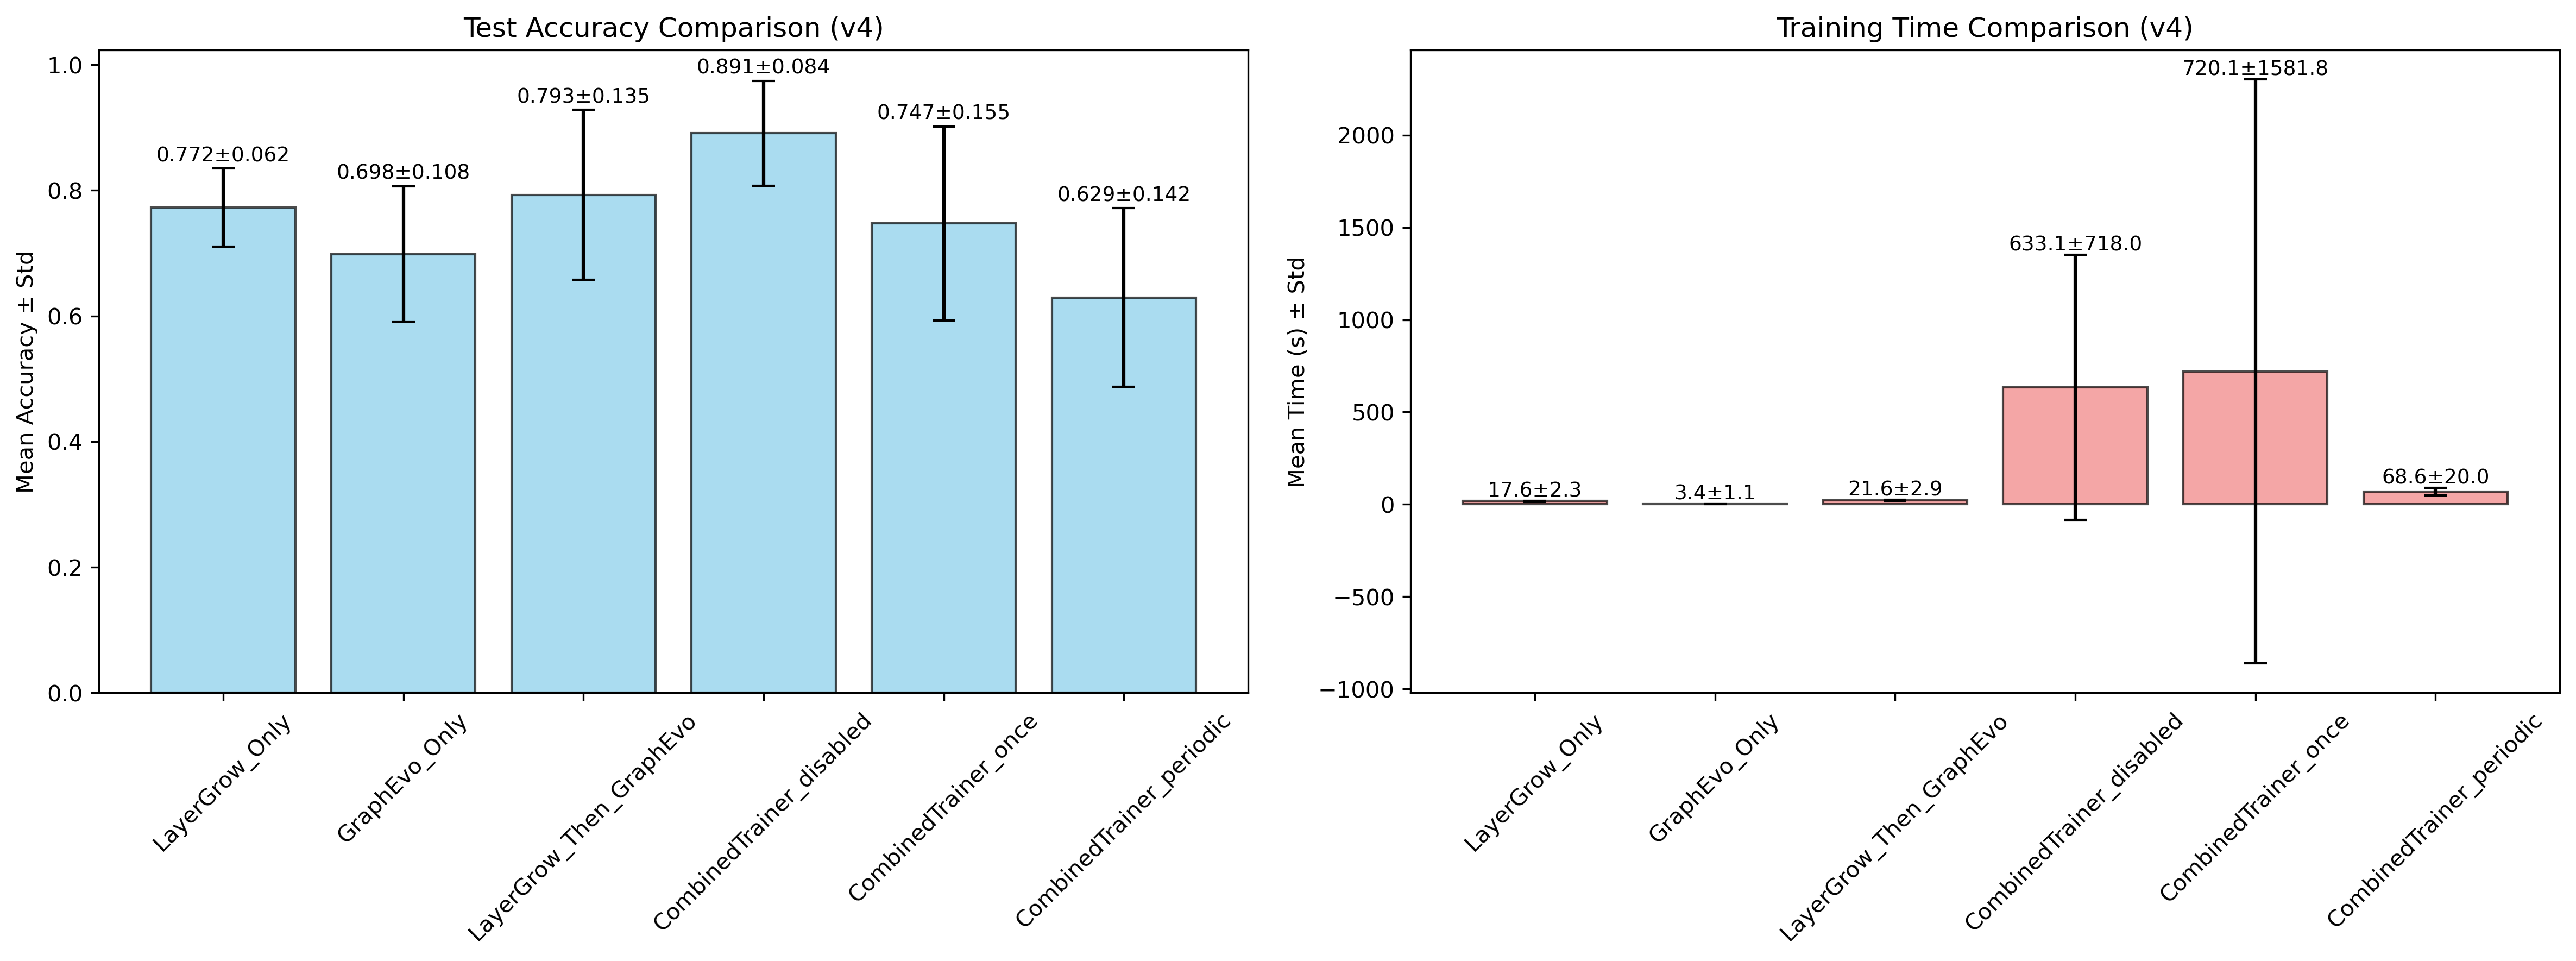
\includegraphics[width=0.95\linewidth]{images/exp_4/exp4_combined_trainer_comparison_circles.png}
\caption{Comparison of Test Accuracy and Training Time for various strategies on the Concentric Circles task (error bars represent standard deviation).}
\label{fig:exp4_circles_comparison}
\end{figure}

\begin{figure}[htbp]
\centering
\begin{minipage}{0.32\linewidth}
    \centering
    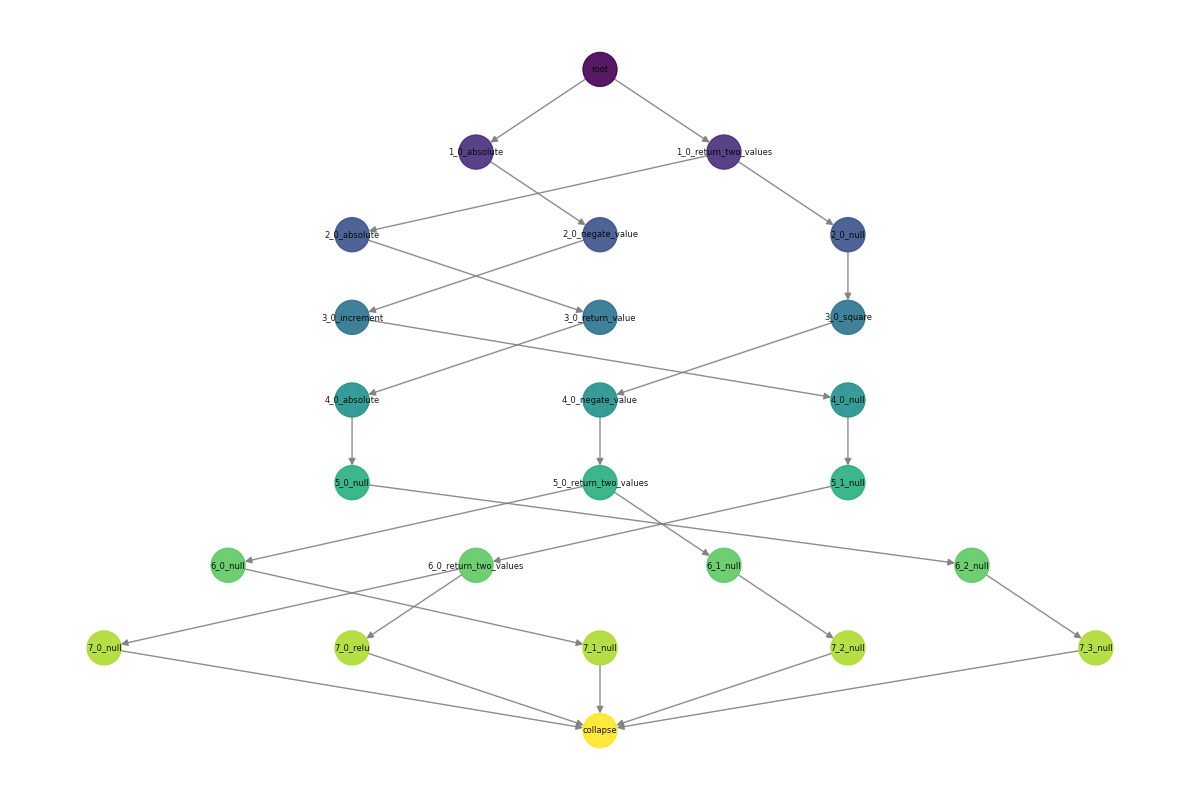
\includegraphics[width=\linewidth]{images/exp_4/circles_best_model_graph.png}

    \textbf{(a) Model Structure}
\end{minipage}
\hfill
\begin{minipage}{0.32\linewidth}
    \centering
    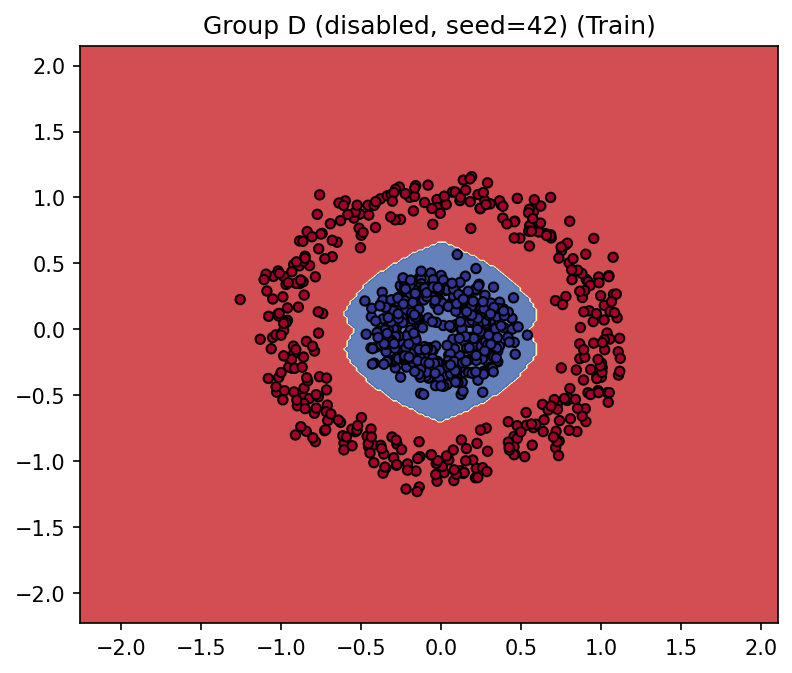
\includegraphics[width=\linewidth]{images/exp_4/circles_best_train.png}

    \textbf{(b) Train Set Boundary}
\end{minipage}
\hfill
\begin{minipage}{0.32\linewidth}
    \centering
    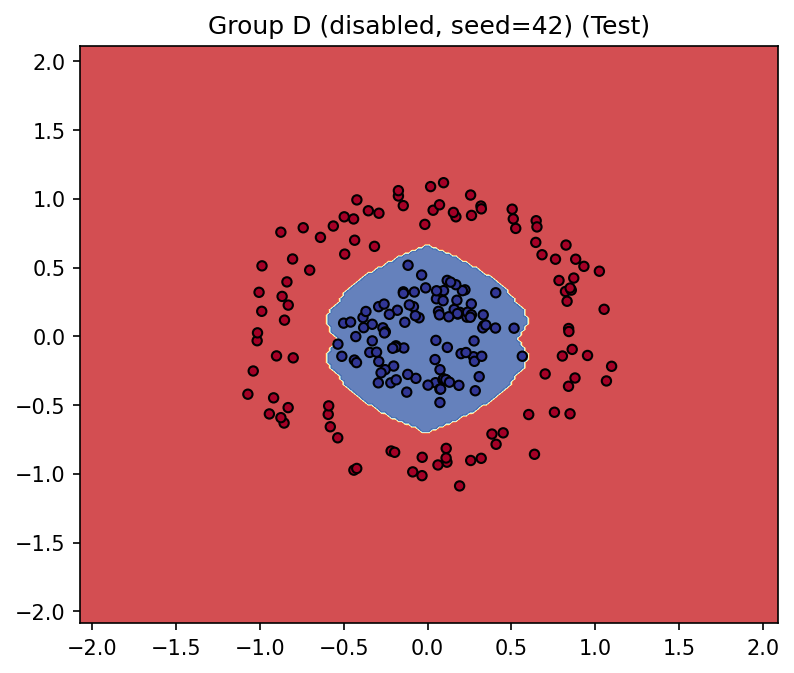
\includegraphics[width=\linewidth]{images/exp_4/circles_best_test.png}

    \textbf{(c) Test Set Boundary}
\end{minipage}
\caption{Structure and decision boundary visualization of the best model from \texttt{CombinedTrainer\_disabled} on the Concentric Circles task. Note the clear square and addition combination logic visible in the structure graph.}
\label{fig:exp4_circles_best_separate}
\end{figure}

\subsubsection*{Two Spirals Task (Full Method Pool)}

This task introduces trigonometric functions to verify the framework's ability to utilize explicit geometric operators.

\begin{table}[htbp]
\centering
\small % 或者 \footnotesize，根据空间情况选择
\setlength{\tabcolsep}{3pt} % 默认是 6pt，减小列间距
\caption{Performance Comparison on Two Spirals Task (Full Pool, 100 repetitions)}
\label{tab:exp_spiral_full}
\begin{tabular}{l c c c c c c}
\toprule
\textbf{Strategy} & \textbf{Test Acc ($\pm$ Std)} & \textbf{Pool Size} & \textbf{Time (s)} & \textbf{\# $\geq$0.99$^*$} & \textbf{Layers} & \textbf{Nodes} \\
\midrule
\textbf{CombinedTrainer\_disabled} & \textbf{0.8493 $\pm$ 0.0338} & 26.0 & 416.4 & \textbf{1} & 6.45 & 20.30 \\
LayerGrow\_Then\_GraphEvo & 0.8148 $\pm$ 0.0556 & 22.0 & 26.5 & 1 & 4.63 & 14.75 \\
LayerGrow\_Only & 0.8053 $\pm$ 0.0389 & 20.0 & 27.4 & 0 & 4.77 & 15.67 \\
CombinedTrainer\_once & 0.7823 $\pm$ 0.0793 & 15.9 & 742.6 & 0 & 6.15 & 20.75 \\
GraphEvo\_Only & 0.7624 $\pm$ 0.0798 & 22.8 & 3.8 & 0 & 3.20 & 8.59 \\
CombinedTrainer\_periodic & 0.7209 $\pm$ 0.1094 & 9.9 & 80.6 & 0 & 4.67 & 16.23 \\
\bottomrule
\multicolumn{7}{l}{\footnotesize $^*$ \textbf{High-Precision Success Count}: Number of runs with Test Accuracy $\geq$ 99\%.}
\end{tabular}
\end{table}

\textbf{Observations:}
\begin{itemize}
    \item Even with powerful operators like \texttt{atan2}, the Two Spirals task remains highly challenging. \texttt{CombinedTrainer\_disabled} still maintained the lead, with an average accuracy of 84.9\%.
    \item Notably, \texttt{CombinedTrainer\_once}, despite having a moderate pool size, had the longest runtime (742.6s) and lower performance than the \texttt{disabled} mode. This may be because after the initial screening, the remaining sub-pool, although streamlined, limited the exploration diversity of new structures in subsequent multi-round evolutions.
    \item \texttt{GraphEvo\_Only} performed better in the Full Pool than in the Restricted Pool (see Table~\ref{tab:exp_spiral_restricted}), indicating that local optimization can more effectively fine-tune node semantics when rich semantic operators are available.
\end{itemize}

\begin{figure}[htbp]
\centering
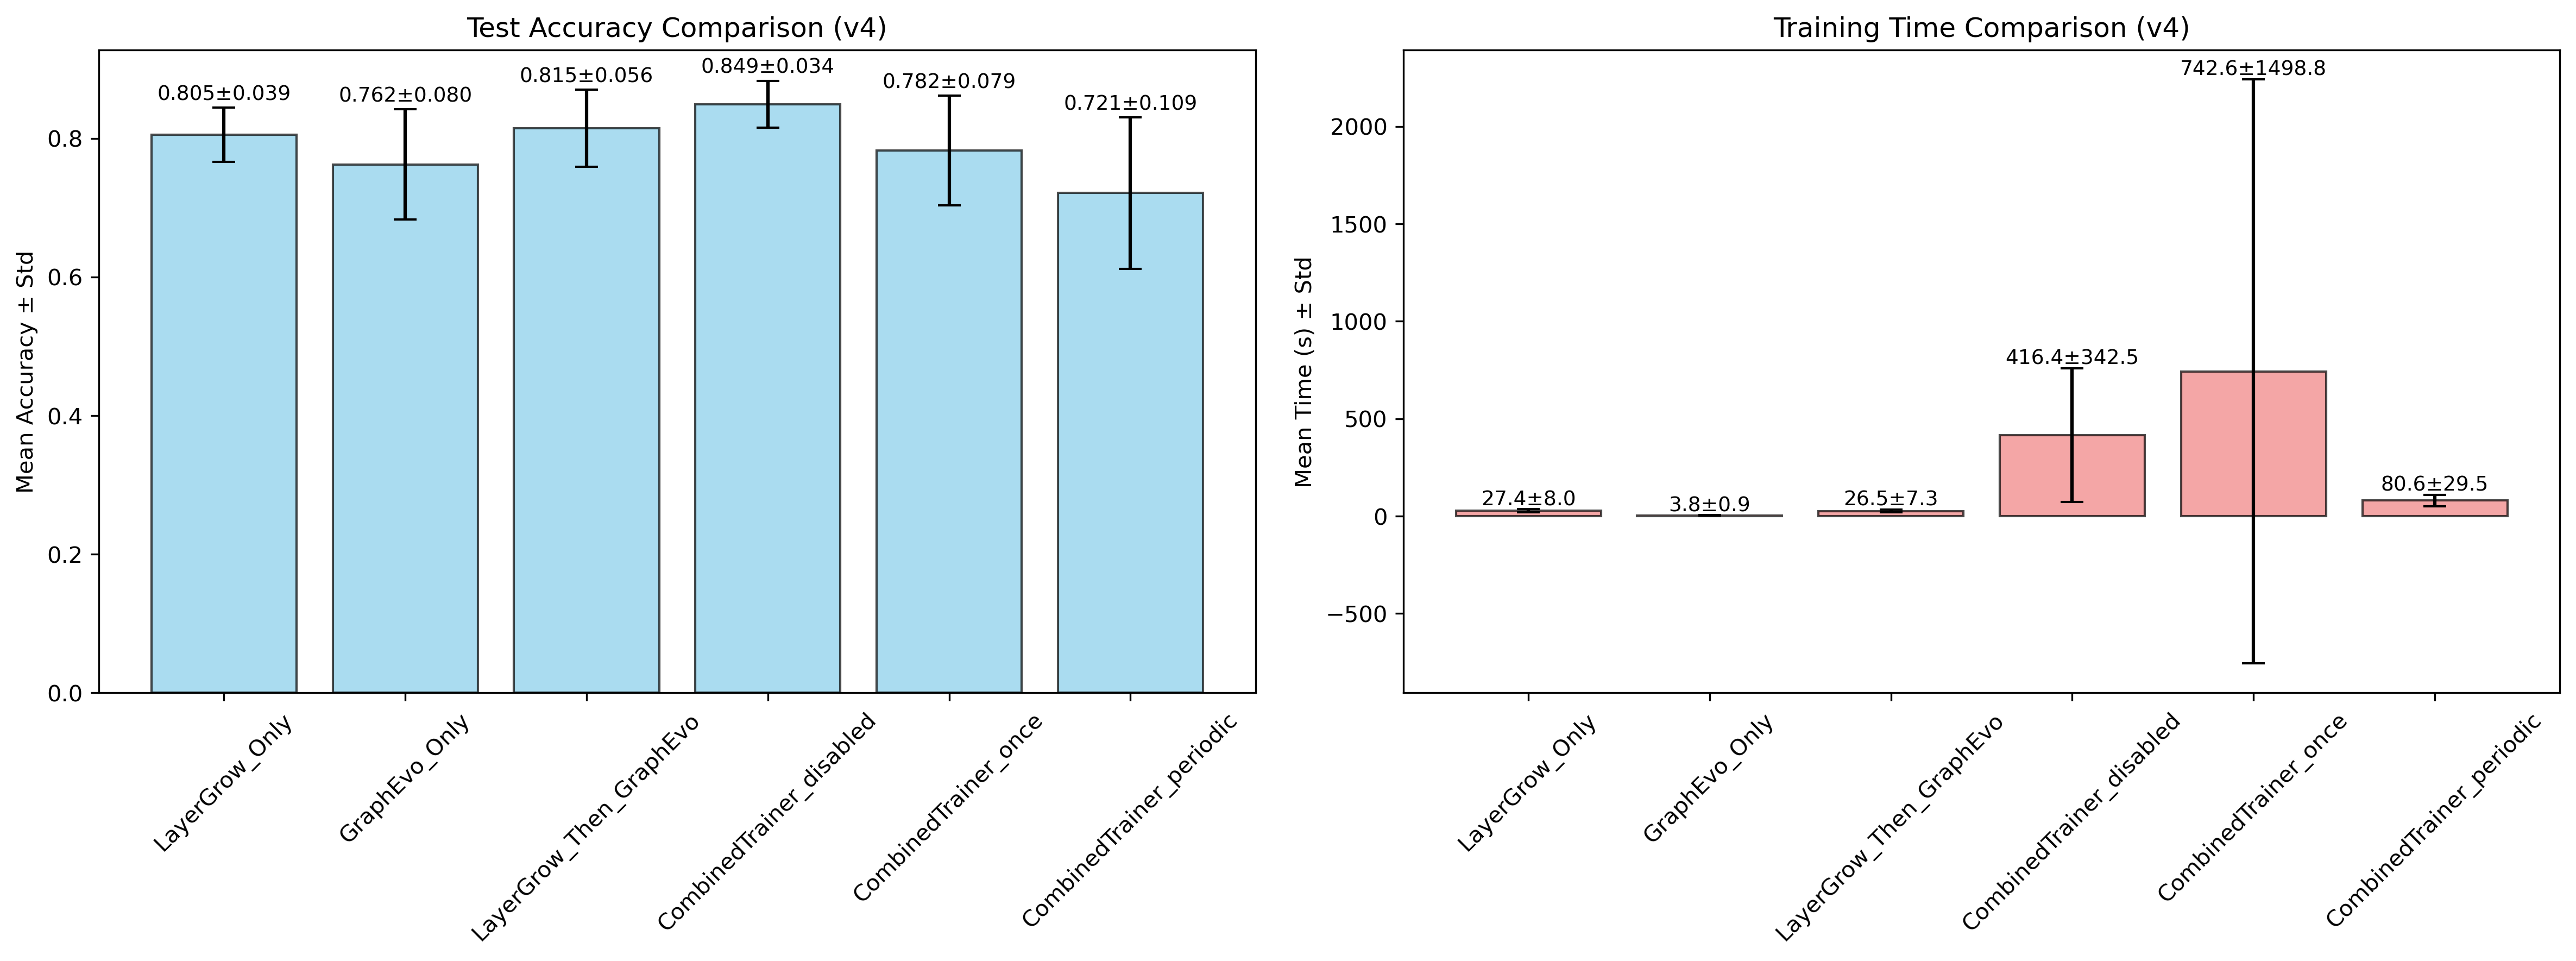
\includegraphics[width=0.95\linewidth]{images/exp_4/exp4_combined_trainer_comparison_spiral.png}
\caption{Performance comparison of various strategies on the Two Spirals task (Full Method Pool).}
\label{fig:exp4_spiral_full_comparison}
\end{figure}

\begin{figure}[htbp]
\centering
\begin{minipage}{0.32\linewidth}
    \centering
    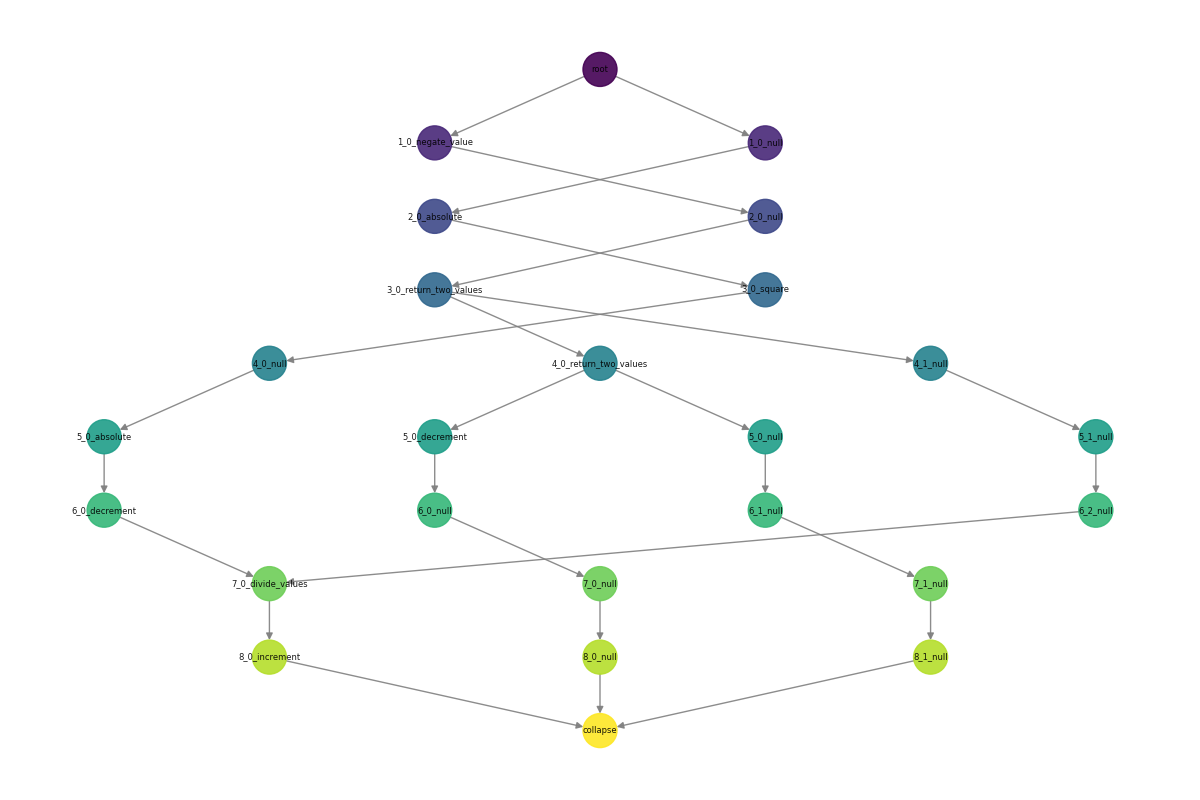
\includegraphics[width=\linewidth]{images/exp_4/spiral_best_model_graph.png}

    \textbf{(a) Model Structure}
\end{minipage}
\hfill
\begin{minipage}{0.32\linewidth}
    \centering
    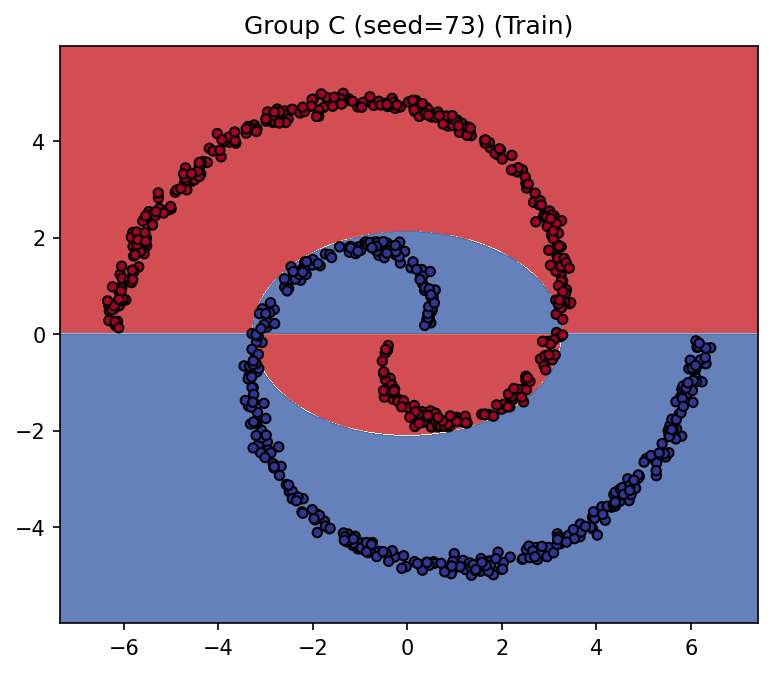
\includegraphics[width=\linewidth]{images/exp_4/spiral_best_train.png}

    \textbf{(b) Train Set Boundary}
\end{minipage}
\hfill
\begin{minipage}{0.32\linewidth}
    \centering
    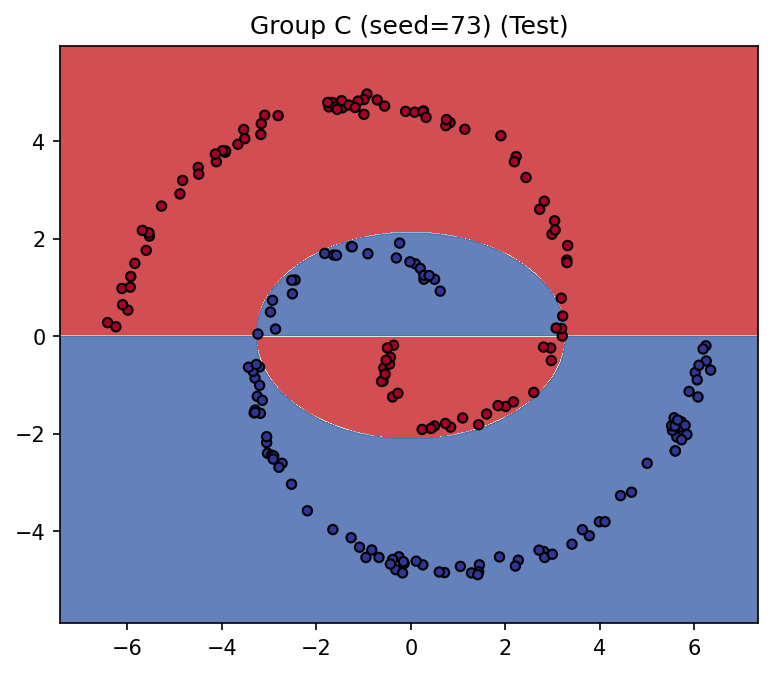
\includegraphics[width=\linewidth]{images/exp_4/spiral_best_test.png}

    \textbf{(c) Test Set Boundary}
\end{minipage}
\caption{Structure and decision boundary visualization of the best model from \texttt{CombinedTrainer\_disabled} on the Two Spirals task (Full Pool). Direct calls to \texttt{atan2} nodes are visible in the structure.}
\label{fig:exp4_spiral_full_best_separate}
\end{figure}

\subsubsection*{Two Spirals Task (Restricted Method Pool)}

This task removes trigonometric functions, forcing the model to approximate spiral boundaries using algebraic operations.

\begin{table}[htbp]
\centering
\small % 或者 \footnotesize，根据空间情况选择
\setlength{\tabcolsep}{3pt} % 默认是 6pt，减小列间距
\caption{Performance Comparison on Two Spirals Task (Restricted Pool, 100 repetitions)}
\label{tab:exp_spiral_restricted}
\begin{tabular}{l c c c c c c}
\toprule
\textbf{Strategy} & \textbf{Test Acc ($\pm$ Std)} & \textbf{Pool Size} & \textbf{Time (s)} & \textbf{\# $\geq$0.99$^*$} & \textbf{Layers} & \textbf{Nodes} \\
\midrule
\textbf{CombinedTrainer\_disabled} & \textbf{0.8386 $\pm$ 0.0390} & 21.0 & 589.3 & \textbf{1} & 6.40 & 22.09 \\
LayerGrow\_Only & 0.8019 $\pm$ 0.0355 & 15.0 & 26.0 & 0 & 5.62 & 20.69 \\
LayerGrow\_Then\_GraphEvo & 0.7989 $\pm$ 0.0421 & 17.0 & 25.2 & 0 & 4.91 & 16.61 \\
CombinedTrainer\_once & 0.7791 $\pm$ 0.0644 & 15.9 & 505.3 & 0 & 5.64 & 20.06 \\
CombinedTrainer\_periodic & 0.7381 $\pm$ 0.0762 & 10.0 & 78.6 & 0 & 4.50 & 14.89 \\
GraphEvo\_Only & 0.7326 $\pm$ 0.0992 & 17.9 & 3.6 & 0 & 3.20 & 8.80 \\
\bottomrule
\multicolumn{7}{l}{\footnotesize $^*$ \textbf{High-Precision Success Count}: Number of runs with Test Accuracy $\geq$ 99\%.}
\end{tabular}
\end{table}

\textbf{Observations:}
\begin{itemize}
    \item Surprisingly, \texttt{CombinedTrainer\_disabled} in the Restricted Pool (83.9\%) showed a minimal performance gap compared to the Full Pool (84.9\%). This demonstrates that AdaptoFlux's \textbf{GDFG structural composition capability} possesses strong expressive redundancy, effectively approximating complex geometric functions through deep algebraic structures.
    \item However, \texttt{GraphEvo\_Only} performance dropped significantly in the Restricted Pool (73.3\% vs 76.2\%), indicating that without high-level semantic operators, relying solely on local node replacement makes it difficult to escape local optima; it must rely on the structural diversity provided by \texttt{LayerGrow}.
\end{itemize}

\begin{figure}[htbp]
\centering
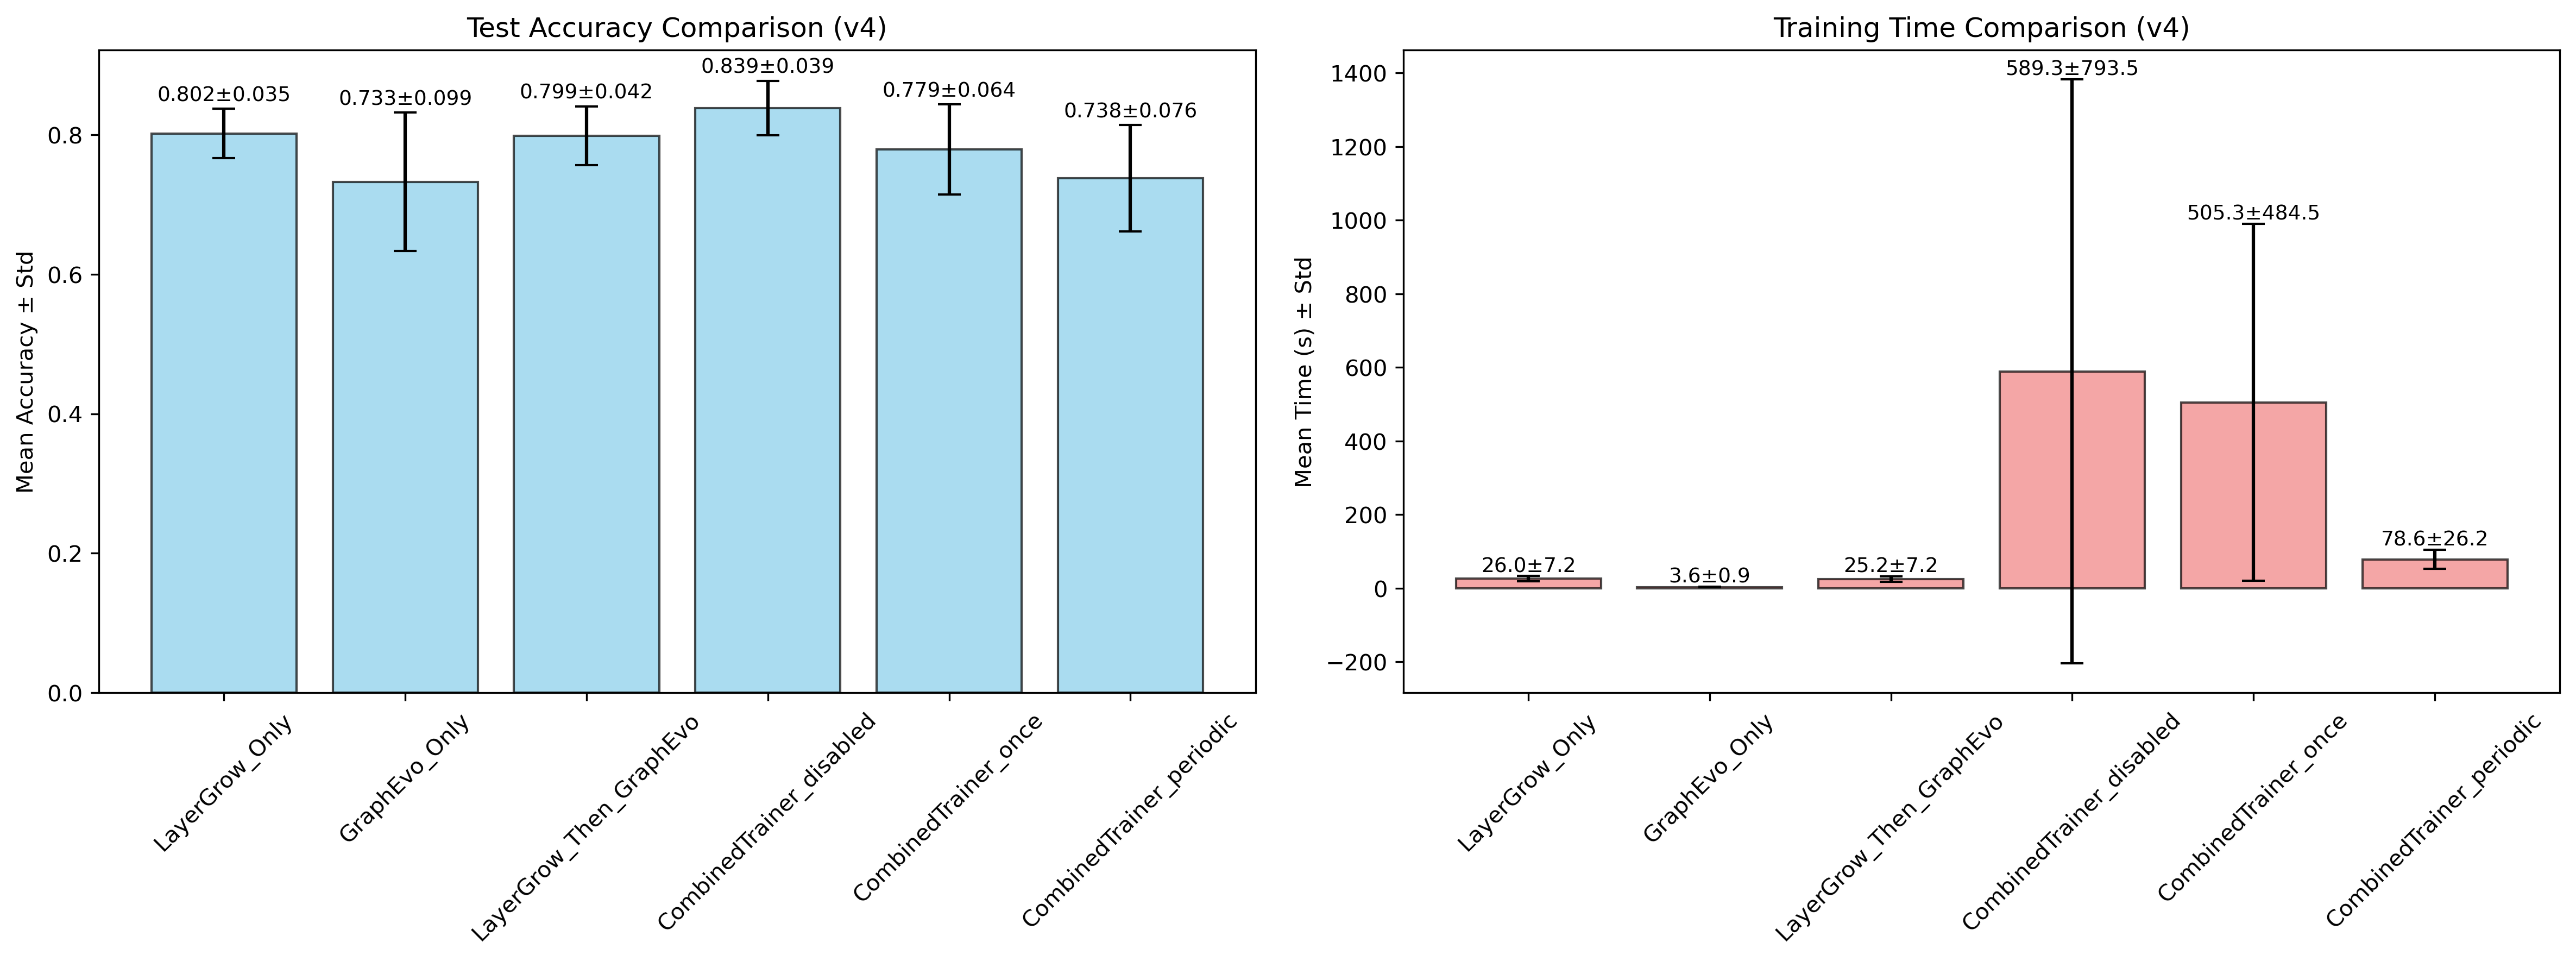
\includegraphics[width=0.95\linewidth]{images/exp_4/exp4_combined_trainer_comparison_spiral_restricted.png}
\caption{Performance comparison of various strategies on the Two Spirals task (Restricted Method Pool).}
\label{fig:exp4_spiral_restricted_comparison}
\end{figure}

\begin{figure}[htbp]
\centering
\begin{minipage}{0.32\linewidth}
    \centering
    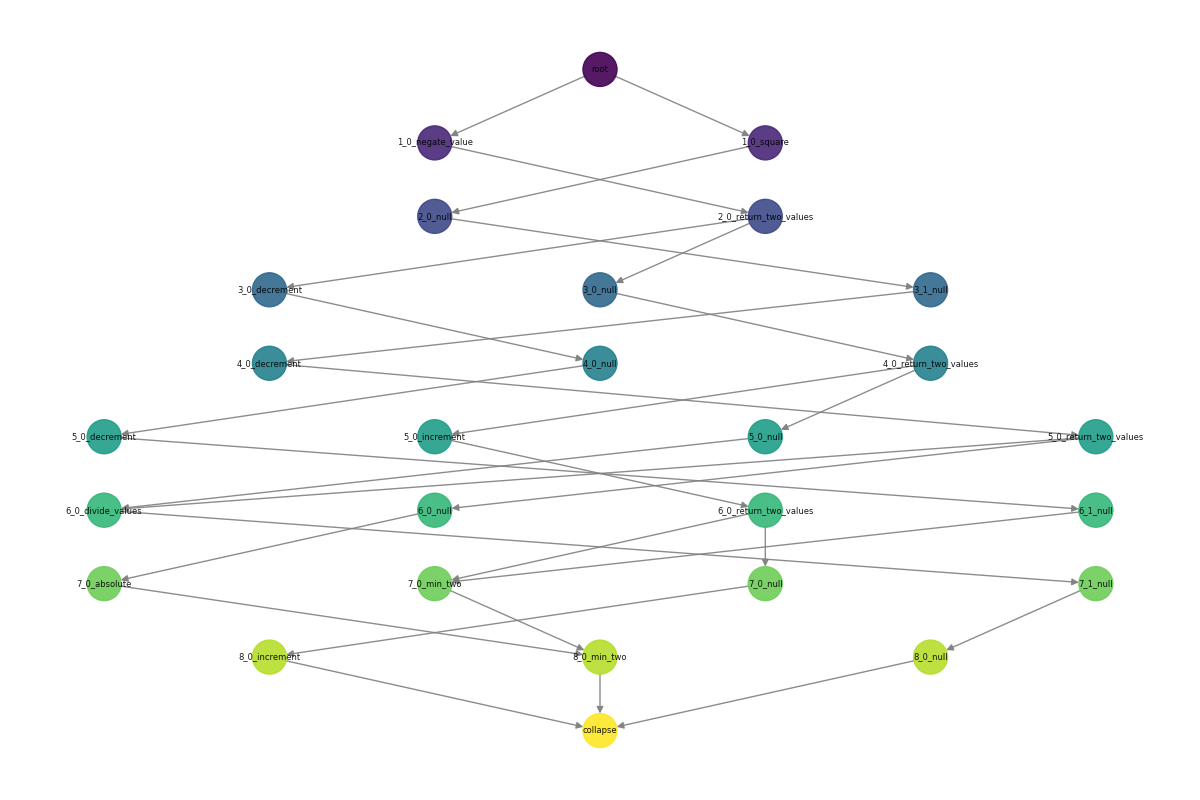
\includegraphics[width=\linewidth]{images/exp_4/spiral_restricted_best_model_graph.png}

    \textbf{(a) Model Structure}
\end{minipage}
\hfill
\begin{minipage}{0.32\linewidth}
    \centering
    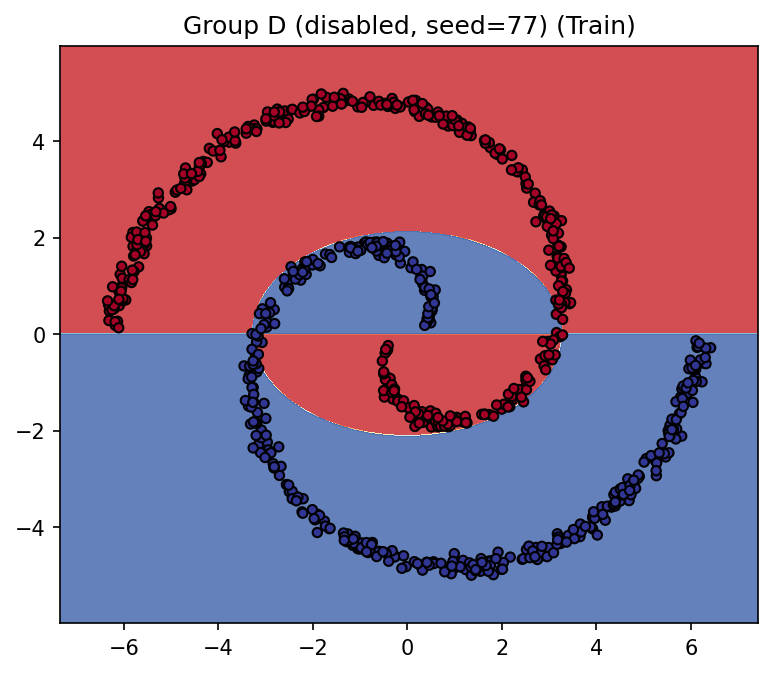
\includegraphics[width=\linewidth]{images/exp_4/spiral_restricted_best_train.png}

    \textbf{(b) Train Set Boundary}
\end{minipage}
\hfill
\begin{minipage}{0.32\linewidth}
    \centering
    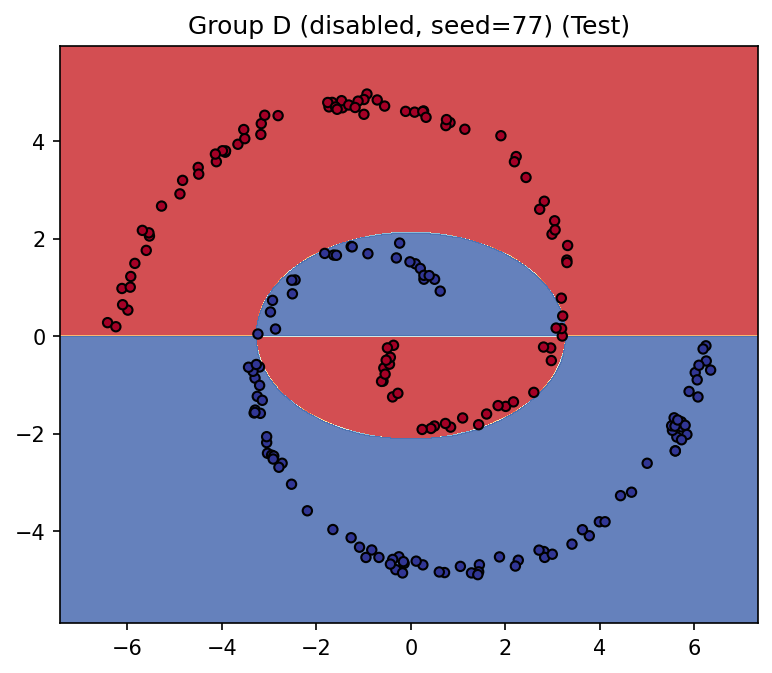
\includegraphics[width=\linewidth]{images/exp_4/spiral_restricted_best_test.png}

    \textbf{(c) Test Set Boundary}
\end{minipage}
\caption{Structure and decision boundary visualization of the best model from \texttt{CombinedTrainer\_disabled} on the Two Spirals task (Restricted Pool). Note that its structure is more complex than the Full Pool model, approximating the spiral shape through multi-layer algebraic operations.}
\label{fig:exp4_spiral_restricted_best_separate}
\end{figure}

\subsection{Analysis and Discussion}

Based on the experimental results above, we draw the following core conclusions:

\begin{itemize}
    \item \textbf{Method Pool Composition Determines Performance Upper Bound, but Structural Composition Can Compensate for Semantic Deficits}
    \begin{itemize}
        \item In the Two Spirals task, the Full Pool slightly outperformed the Restricted Pool, verifying the natural advantage of geometric operators like \texttt{atan2}/\texttt{sin}/\texttt{cos} for polar coordinate tasks.
        \item However, the gap was not substantial ($\sim$1\%), and high-precision solutions were still obtained in the Restricted Pool. This proves that AdaptoFlux's GDFG structural composition capability has strong expressive redundancy, capable of approximating complex geometric functions through deep algebraic structures.
    \end{itemize}
    
    \item \textbf{Multi-Round Combination (Disabled) Outperforms Single-Round and Over-Screening}
    \begin{itemize}
        \item \texttt{CombinedTrainer\_disabled} achieved the best average performance and high-precision success rate in all tasks. Through 3 rounds of ``LayerGrow $\rightarrow$ GraphEvo'' cycles, the model could gradually deepen the structure and refine semantics, proving the effectiveness of \textbf{deep structural exploration}.
        \item In contrast, \texttt{LayerGrow\_Then\_GraphEvo} (single-round) was significantly inferior to the multi-round mode due to the depth limit of single growth.
    \end{itemize}
    
    \item \textbf{Genetic Screening is a Double-Edged Sword: Diversity vs. Efficiency}
    \begin{itemize}
        \item \texttt{CombinedTrainer\_periodic} performed the worst in all tasks. Although it significantly reduced the method pool size (to $\sim$10) and shortened single-round time, \textbf{over-compression led to the loss of key nonlinear operations (such as \texttt{square}, \texttt{atan2}) or critical intermediate combinations}.
        \item In geometrically sensitive tasks, \textbf{preserving method pool diversity is more important than streamlining the search space}. Genetic screening mechanisms should be used with caution; it is recommended to prioritize \texttt{disabled} or \texttt{once} modes when tasks are highly sensitive to specific atomic operations to avoid premature pruning of the search space.
    \end{itemize}
    
    \item \textbf{Complementarity of Layered Growth and Graph Evolution}
    \begin{itemize}
        \item \texttt{LayerGrow\_Then\_GraphEvo} outperformed separate \texttt{LayerGrow\_Only} or \texttt{GraphEvo\_Only} in all tasks.
        \item \texttt{LayerGrow} is responsible for expanding the \textbf{macro-topological depth} of the structure, solving the problem of ``whether it can be represented''; \texttt{GraphEvo} is responsible for \textbf{micro-semantic alignment}, solving the problem of ``how accurately it is represented''. The synergy of the two is the core driving force for AdaptoFlux to navigate discrete spaces.
    \end{itemize}
    
    \item \textbf{Strong Interpretability and Symbolic Nature}
    \begin{itemize}
        \item As shown in Figures \ref{fig:exp4_circles_best_separate}, \ref{fig:exp4_spiral_full_best_separate}, and \ref{fig:exp4_spiral_restricted_best_separate}, the generated GDFG structures are clear and sparse. The mathematical expression of the decision logic can be directly deduced from the model structure graph (e.g., the $x_1^2 + x_2^2$ combination in the Concentric Circles task, or the \texttt{atan2} call in the Two Spirals task).
        \item This \textbf{white-box characteristic} is the essential advantage of AdaptoFlux as a symbolic-structural hybrid paradigm, giving it potential application value in scientific computing and control fields requiring high credibility.
    \end{itemize}
\end{itemize}

\subsection{Conclusion}

The experiments in this appendix demonstrate that AdaptoFlux exhibits powerful structural composition capabilities in complex geometric tasks. Its performance depends not only on the \textbf{completeness} of the method pool but also on the balance between \textbf{structural depth} and \textbf{semantic diversity} maintained by the training strategy.

For practical applications, we recommend:
\begin{itemize}
    \item When exploring unknown complex tasks, prioritize using \textbf{\texttt{CombinedTrainer\_disabled}} to maximize the exploration space.
    \item If computational resources are limited and the task semantics are known, try \textbf{\texttt{CombinedTrainer\_once}} for moderate compression.
    \item Avoid using high-frequency periodic genetic screening (\texttt{periodic}) in the early stages to prevent destroying the connectivity of the solution space.
\end{itemize}

\section{Static Symbolic Regression with Restricted Method Pools}
\label{sec:appendix_baseline_comparison}

We compare the original AdaptoFlux probes with PySR and gplearn on eight Feynman formulas, using the four arithmetic primitives listed below. The experiment measures formula recovery, numerical accuracy and sensitivity to output aggregation. All results use numerical operators; stateful execution is evaluated separately in Sections~\ref{subsec:stateful_synthesis} and \ref{app:revision_action}.

\subsection{Tasks and Restricted Experimental Setting}

The eight target formulas are:
\begin{align*}
    f_1(m, c) &= m \cdot c^2 & \text{(Energy)} \\
    f_2(m, a) &= m \cdot a & \text{(Newton's Second Law)} \\
    f_3(m, v) &= 0.5 \cdot m \cdot v^2 & \text{(Kinetic Energy)} \\
    f_4(q_1, q_2, r) &= \frac{q_1 q_2}{r^2} & \text{(Coulomb's Law)} \\
    f_5(n, T, V) &= \frac{n T}{V} & \text{(Ideal Gas Law)} \\
    f_6(I, R) &= I \cdot R & \text{(Ohm's Law)} \\
    f_7(v_1, v_2, t) &= \frac{v_2 - v_1}{t} & \text{(Acceleration Definition)} \\
    f_8(V, I) &= V \cdot I & \text{(Electric Power)}
\end{align*}

The common mathematical primitives are \texttt{add}, \texttt{sub}, \texttt{mul}, \texttt{div}.
AdaptoFlux's layer-building interface also supplies \texttt{fanout} (variable copying) and \texttt{identity} (passthrough). These auxiliary methods support reuse in that particular construction interface; variable reuse is also intrinsic to a general DAG through multiple outgoing edges. Output aggregation is a further experimental configuration, varied among \texttt{first}, \texttt{prod} and \texttt{sum} below.

\textbf{Deliberately Restricted Setting (a sanity check, not a race)}: Because gplearn and PySR are pure-symbolic tools that cannot exercise AdaptoFlux's method imports, we \textbf{actively disabled ATF's method-import capability}, reducing it to a pure symbolic synthesizer using only 5 basic operators. This isolates the expressiveness of the representation itself (graph structure vs.\ tree/expression) from differences in function sets, rather than staging a head-to-head comparison of search engines. The experiment therefore probes a lower bound on what the GDFG substrate can express under the current probes; it is not the operating mode for which AdaptoFlux is designed.

\subsection{Experimental Setup}

All methods were run independently 10 times on each task with different random seeds. This experiment reports the \textbf{best-of-10 MSE, Exact Match status (Exact?), runtime (seconds), and final method pool size}. AdaptoFlux was tested with three different \texttt{collapse\_mode} strategies:
\begin{description}
    \item[\texttt{first}] First valid output;
    \item[\texttt{prod}] Product aggregation;
    \item[\texttt{sum}] Sum aggregation.
\end{description}

Baseline methods include:
\begin{description}
    \item[\textbf{gplearn}] Classic Genetic Programming implementation, using the same 5-function set;
    \item[\textbf{PySR}] Modern symbolic regression tool based on sparse regression and symbolic enumeration;
    \item[\textbf{XGBoost}] Black-box gradient boosting tree model, used to contrast pure predictive performance with interpretability trade-offs.
\end{description}

To more accurately assess \textbf{program equivalence} in symbolic regression tasks, this experiment adopts a \textbf{numerical-symbolic joint discrimination strategy}. Specifically, we first determine if the model output is numerically highly consistent with the ground truth using the following function:
\begin{lstlisting}[language=Python, basicstyle=\small\ttfamily]
def is_numerical_exact_match(y_pred, y_true, tol=1e-5):
    return np.all(np.abs(y_pred - y_true) < tol)
\end{lstlisting}
This function requires the prediction error for all test samples to be strictly less than $10^{-5}$. However, relying solely on MSE or numerical matching may yield \textbf{false positives} (e.g., the model fits an expression that looks similar but is structurally incorrect) or \textbf{false negatives} (e.g., high MSE due to constant offset but correct structure). Therefore, in addition to automatic judgment, we further performed \textbf{manual symbolic parsing verification} on the \textbf{best expressions} output by ATF, gplearn, and PySR to confirm whether they are \textbf{algebraically equivalent} to the target formula (e.g., $x_0 \cdot x_1 \cdot x_1$ is equivalent to $m \cdot c^2$ under variable mapping).

Based on this dual verification mechanism, we constructed Table~\ref{tab:symbolic_exact_match}, which specifically records whether each method \textbf{truly recovered the target physical formula at the symbolic level}.

\subsection{Results Overview}

Tables~\ref{tab:baselines_first}--\ref{tab:baselines_sum} present the best-of-10 performance of AdaptoFlux under the three collapse modes; Table~\ref{tab:baselines_gp_pysr} summarizes the corresponding results for gplearn, PySR, and XGBoost; and Table~\ref{tab:symbolic_exact_match} reports the symbolic-level exact match analysis. Best-of-10 tables are retained only because this is how the reference systems are conventionally reported on this suite; stability-oriented conclusions rely on the mean $\pm$ std statistics in Tables~\ref{tab:atf_stats_first}--\ref{tab:atf_stats_sum} and Figures~\ref{fig:mse_distribution}--\ref{fig:success_rate}.

Key findings are as follows:
\begin{itemize}
    \item \textbf{gplearn and PySR achieved exact matches (Exact?=Yes) on most tasks}, with MSE typically below $10^{-12}$, performing robustly especially in binary multiplication or simple division tasks (e.g., F\_ma, OhmsLaw, Acceleration, Power, Coulomb)---as expected for systems specialized in exactly this static setting.
    \item \textbf{XGBoost failed to recover analytical expressions}, with MSE generally 2--4 orders of magnitude higher, highlighting its fundamental limitations in symbolic recovery tasks.
    \item \textbf{AdaptoFlux's performance is highly dependent on the collapse mode}:
        \begin{itemize}
            \item The \texttt{prod} mode performed best in multiplication-dominated tasks (F\_ma, OhmsLaw, Power, E\_mc2, KE), achieving exact matches (MSE $\sim 10^{-13}$) for F\_ma, OhmsLaw, and Power, comparable to gplearn/PySR;
            \item The \texttt{first} mode succeeded in some tasks (e.g., F\_ma) but exhibited poorer overall stability;
            \item The \texttt{sum} mode generally performed worst, barely reaching high precision only in OhmsLaw and Power.
        \end{itemize}
    \item \textbf{Complex tasks remain a bottleneck for the current probes}: for tasks involving explicit constants (e.g., 0.5 in KE) or three-variable nonlinear combinations (IdealGas, Coulomb), the restricted ATF failed to recover the exact formula, with MSE significantly higher than the specialized reference systems. As analyzed below, this reflects the limits of the lightweight local-search probes under a fixed uniform configuration rather than a representational deficit.
    \item \textbf{Native action support is not exercised here}: the ``Supports actions'' markers in the tables record only that the execution backend accepts side-effecting methods; that capability is deliberately disabled in this section and is demonstrated separately by the automatic stateful synthesis experiment (Section~\ref{subsec:stateful_synthesis}) and the Snake case study (Appendix~\ref{app:snake_controller}).
\end{itemize}

We tested three collapse modes, with \texttt{prod} performing best in multiplication-dominated tasks; thus, subsequent analysis focuses primarily on this mode.

\begin{table}[htbp]
\centering
\caption{Parameter-free symbolic regression with collapse=first (best of 10 runs)}
\label{tab:baselines_first}
\begin{tabular}{lccccc}
\toprule
Task & Exact? & MSE & Runtime (s) & Method Pool & Notes \\
\midrule
E\_mc2 & No & 2e+03 & 4.0 & 5 & Supports actions \\
F\_ma & \textbf{Yes} & 3e-12 & 0.3 & 5 & Supports actions \\
KE & No & 4e+03 & 42.0 & 8 & Supports actions \\
Coulomb & No & 1e+01 & 13.1 & 7 & Supports actions \\
IdealGas & No & 3e+04 & 11.0 & 7 & Supports actions \\
OhmsLaw & \textbf{Yes} & 5e-13 & 0.4 & 5 & Supports actions \\
Acceleration & No & 7e+00 & 10.7 & 7 & Supports actions \\
Power & \textbf{Yes} & 1e-12 & 0.4 & 5 & Supports actions \\
\bottomrule
\end{tabular}
\end{table}

\begin{table}[htbp]
\centering
\caption{AdaptoFlux performance with \texttt{collapse=prod} (best of 10 runs). 
The ``Exact?'' column indicates \textbf{numerical exact match}: all absolute errors on the test set are $< 10^{-5}$. 
This is stricter than $\mathrm{MSE} < 10^{-5}$ and does not imply symbolic equivalence.}
\label{tab:baselines_prod}
\begin{tabular}{lccccc}
\toprule
Task & Exact? & MSE & Runtime (s) & Method Pool & Notes \\
\midrule
E\_mc2 & No & 2e-11 & 0.1 & 5 & Supports actions \\
F\_ma & \textbf{Yes} & 2e-13 & 0.0 & 5 & Supports actions \\
KE & No & 2e-11 & 0.1 & 5 & Supports actions \\
Coulomb & No & 9e+00 & 6.0 & 5 & Supports actions \\
IdealGas & No & 2e+04 & 19.8 & 8 & Supports actions \\
OhmsLaw & \textbf{Yes} & 2e-13 & 0.0 & 5 & Supports actions \\
Acceleration & No & 5e+00 & 11.2 & 7 & Supports actions \\
Power & \textbf{Yes} & 8e-13 & 0.0 & 5 & Supports actions \\
\bottomrule
\end{tabular}
\end{table}

\begin{table}[htbp]
\centering
\caption{Parameter-free symbolic regression with collapse=sum (best of 10 runs)}
\label{tab:baselines_sum}
\begin{tabular}{lccccc}
\toprule
Task & Exact? & MSE & Runtime (s) & Method Pool & Notes \\
\midrule
E\_mc2 & No & 8e+00 & 532.1 & 8 & Supports actions \\
F\_ma & No & 4e+01 & 6.4 & 7 & Supports actions \\
KE & No & 8e+02 & 39.9 & 8 & Supports actions \\
Coulomb & No & 1e+01 & 8.6 & 6 & Supports actions \\
IdealGas & No & 3e+04 & 2.2 & 5 & Supports actions \\
OhmsLaw & \textbf{Yes} & 1e-12 & 0.5 & 5 & Supports actions \\
Acceleration & No & 1e+01 & 9.7 & 6 & Supports actions \\
Power & \textbf{Yes} & 2e-12 & 1.6 & 5 & Supports actions \\
\bottomrule
\end{tabular}
\end{table}

\begin{table}[htbp]
\centering
\caption{Baseline performance of gplearn, PySR, and XGBoost (best of 10 runs)}
\label{tab:baselines_gp_pysr}
\begin{tabular}{lcccc}
\toprule
Task & Method & Exact? & MSE & Runtime (s) \\
\midrule
\multirow{3}{*}{E\_mc2}
& Gplearn & \textbf{Yes} & 8.3e-12 & 17.86 \\
& PySR & \textbf{Yes} & 8.3e-12 & 20.29 \\
& Xgboost & No & 1.5e+02 & 0.04 \\
\midrule
\multirow{3}{*}{F\_ma}
& Gplearn & \textbf{Yes} & 1.9e-13 & 16.40 \\
& PySR & \textbf{Yes} & 2.1e-12 & 20.49 \\
& Xgboost & No & 2.5e+01 & 724.38 \\
\midrule
\multirow{3}{*}{KE}
& Gplearn & No & 3.4e-11 & 72.71 \\
& PySR & No & 3.4e-11 & 20.31 \\
& Xgboost & No & 3.9e+02 & 0.03 \\
\midrule
\multirow{3}{*}{Coulomb}
& Gplearn & \textbf{Yes} & 6.8e-14 & 10.49 \\
& PySR & \textbf{Yes} & 2.7e-13 & 20.46 \\
& Xgboost & No & 6.4 & 0.02 \\
\midrule
\multirow{3}{*}{IdealGas}
& Gplearn & No & 1e-10 & 122.72 \\
& PySR & No & 2.2e-10 & 20.32 \\
& Xgboost & No & 4.5e+03 & 0.05 \\
\midrule
\multirow{3}{*}{OhmsLaw}
& Gplearn & \textbf{Yes} & 2.2e-13 & 9.24 \\
& PySR & \textbf{Yes} & 2.2e-13 & 20.40 \\
& Xgboost & No & 9.6 & 0.03 \\
\midrule
\multirow{3}{*}{Acceleration}
& Gplearn & \textbf{Yes} & 3.9e-14 & 28.84 \\
& PySR & \textbf{Yes} & 1.1e-13 & 20.46 \\
& Xgboost & No & 1.7 & 0.04 \\
\midrule
\multirow{3}{*}{Power}
& Gplearn & \textbf{Yes} & 8e-13 & 116.68 \\
& PySR & \textbf{Yes} & 1e-12 & 20.20 \\
& Xgboost & No & 3.1e+01 & 0.03 \\
\bottomrule
\end{tabular}
\end{table}

\begin{table}[htbp]
\small % 或者 \footnotesize，根据空间情况选择
\setlength{\tabcolsep}{3pt} % 默认是 6pt，减小列间距
\centering
\caption{Symbolic expressions recovered by gplearn and PySR}
\label{tab:symbolic_expressions}
\begin{tabularx}{\linewidth}{@{}lc>{\raggedright\arraybackslash}Xc@{}}
\toprule
Task & Method & Expression & Exact? \\
\midrule
\multirow{2}{*}{E\_mc2}
& gplearn & \texttt{mul(mul(X1, X0), X1)}  & \textbf{Yes} \\
& PySR & \texttt{x0*x1*x1}  & \textbf{Yes} \\
\midrule
\multirow{2}{*}{F\_ma}
& gplearn & \texttt{mul(X0, X1)} & \textbf{Yes} \\
& PySR & \texttt{x0*x1 - 0.027047554 - 1*(-0.027047586)} & \textbf{No} \\
\midrule
\multirow{2}{*}{KE}
& gplearn & \texttt{mul(mul(X2, X1), mul(X0, X1))} & \textbf{Yes} \\
& PySR & \texttt{x0*x1*x1*x2} & \textbf{Yes} \\
\midrule
\multirow{2}{*}{Coulomb}
& gplearn & \texttt{div(mul(div(X1, X2), X0), X2)} & \textbf{Yes} \\
& PySR & \path{x0/((x2/((x1/x2))))} & \textbf{Yes} \\
\midrule
\multirow{2}{*}{IdealGas}
& gplearn & \texttt{div(X1, div(X2, X0))} & \textbf{Yes} \\
& PySR & \path{x0*x1/x2} & \textbf{Yes} \\
\midrule
\multirow{2}{*}{OhmsLaw}
& gplearn & \texttt{mul(X0, X1)} & \textbf{Yes} \\
& PySR & \texttt{x0*x1 - (-x0 + x0 - x1 + x1)} & \textbf{Yes} \\
\midrule
\multirow{2}{*}{Acceleration}
& gplearn & \texttt{div(sub(X1, X0), X2)} & \textbf{Yes} \\
& PySR & \path{(-x0 + x1 - 6.078859e-6/(x2/((x2/(-16.520508)))))/x2} & \textbf{No} \\
\midrule
\multirow{2}{*}{Power}
& gplearn & \texttt{mul(X1, X0)} & \textbf{Yes} \\
& PySR & \texttt{x1*(x0 - 1*0.99999976) + x1} & \textbf{No} \\
\bottomrule
\end{tabularx}
\end{table}

\begin{figure}[p] % [p] 表示独占一页 (Page)
\centering
% 主标题稍微精简，避免占用过多垂直空间
\caption{Best computation graphs generated by AdaptoFlux on eight Feynman formula tasks. Yes/No indicates algebraic equivalence (see Table~\ref{tab:symbolic_exact_match}).}
\label{fig:atf_graphs}

% 使用 \resizebox 或者手动控制每个图片的高度
% 这里我们假设每行两个图片，共4行。
% 为了安全起见，我们限制每个图片的最大高度为 \textheight 的 1/5 (因为还有标题和间距)

% --- Row 1 ---
\begin{minipage}{0.48\linewidth}
  \centering
  % height=0.18\textheight: 4行图片 + 间距 + 标题 ≈ 0.72 + 0.1 = 0.82 < 0.9
  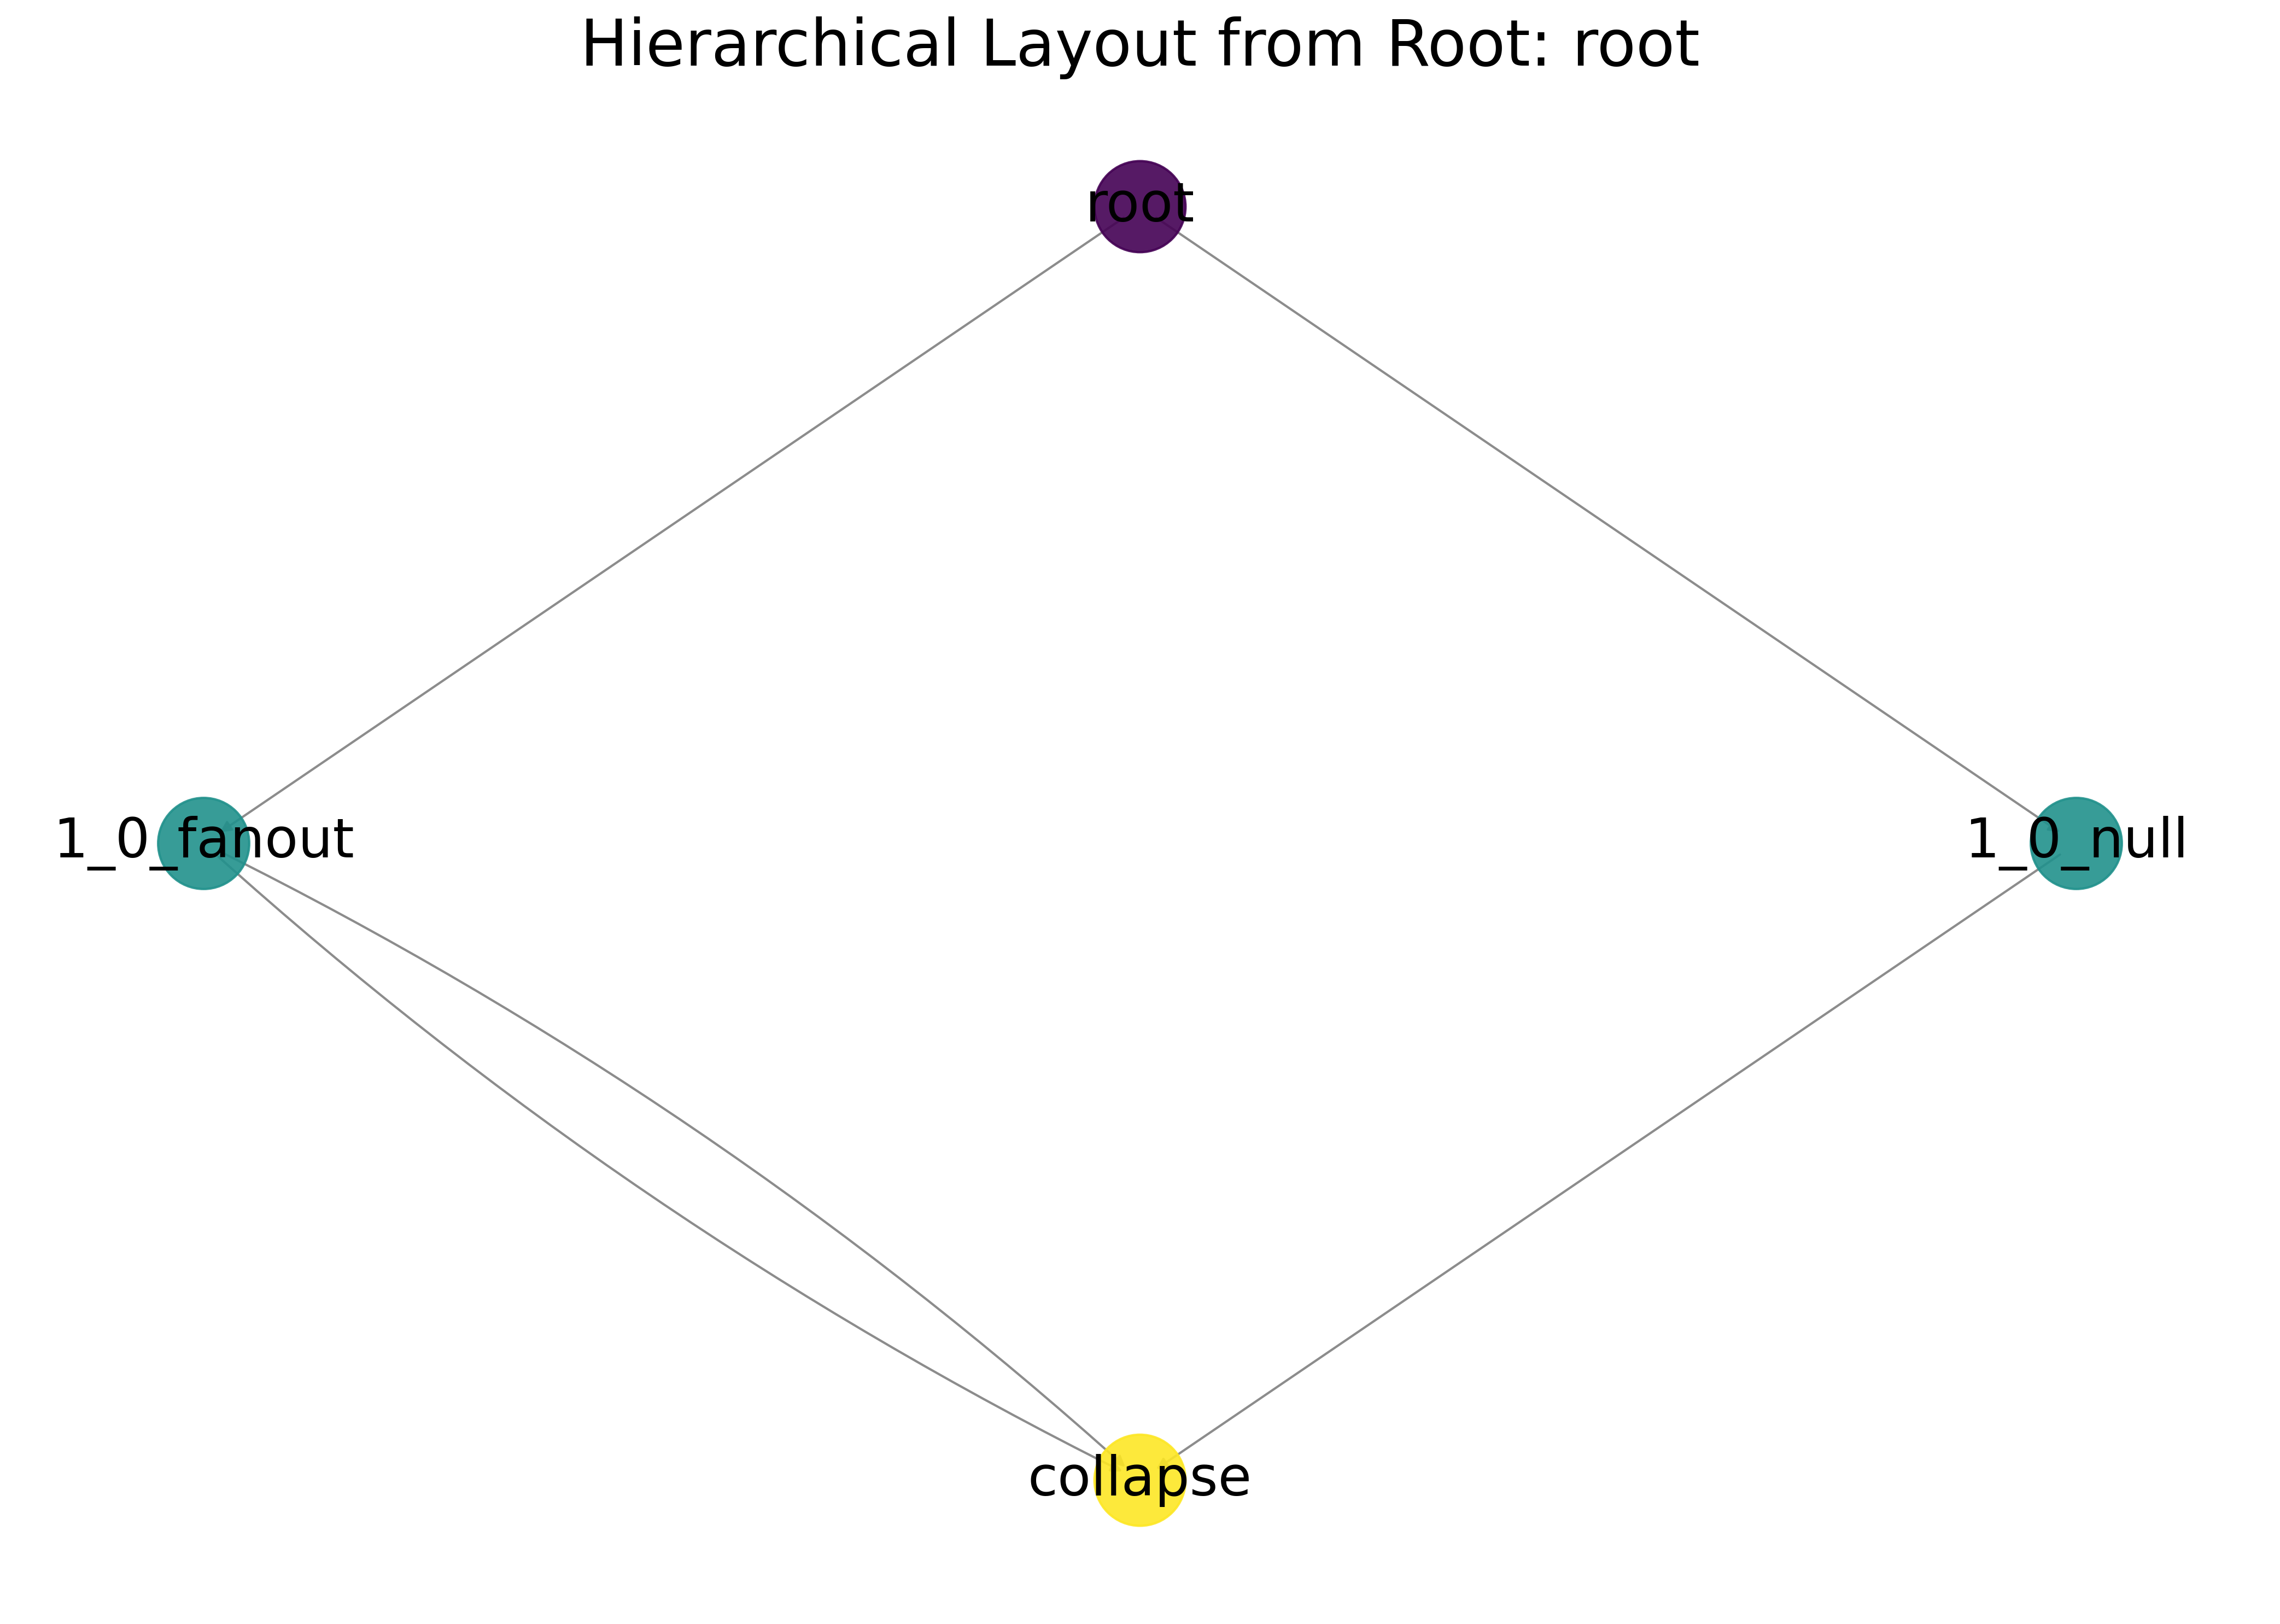
\includegraphics[width=\linewidth, height=0.18\textheight, keepaspectratio]{images/ExternalBaselines/best_E_mc2_collapse_prod.png}

  {\small\textbf{(a)} E\_mc2 (Yes)}
\end{minipage}
\hfill
\begin{minipage}{0.48\linewidth}
  \centering
  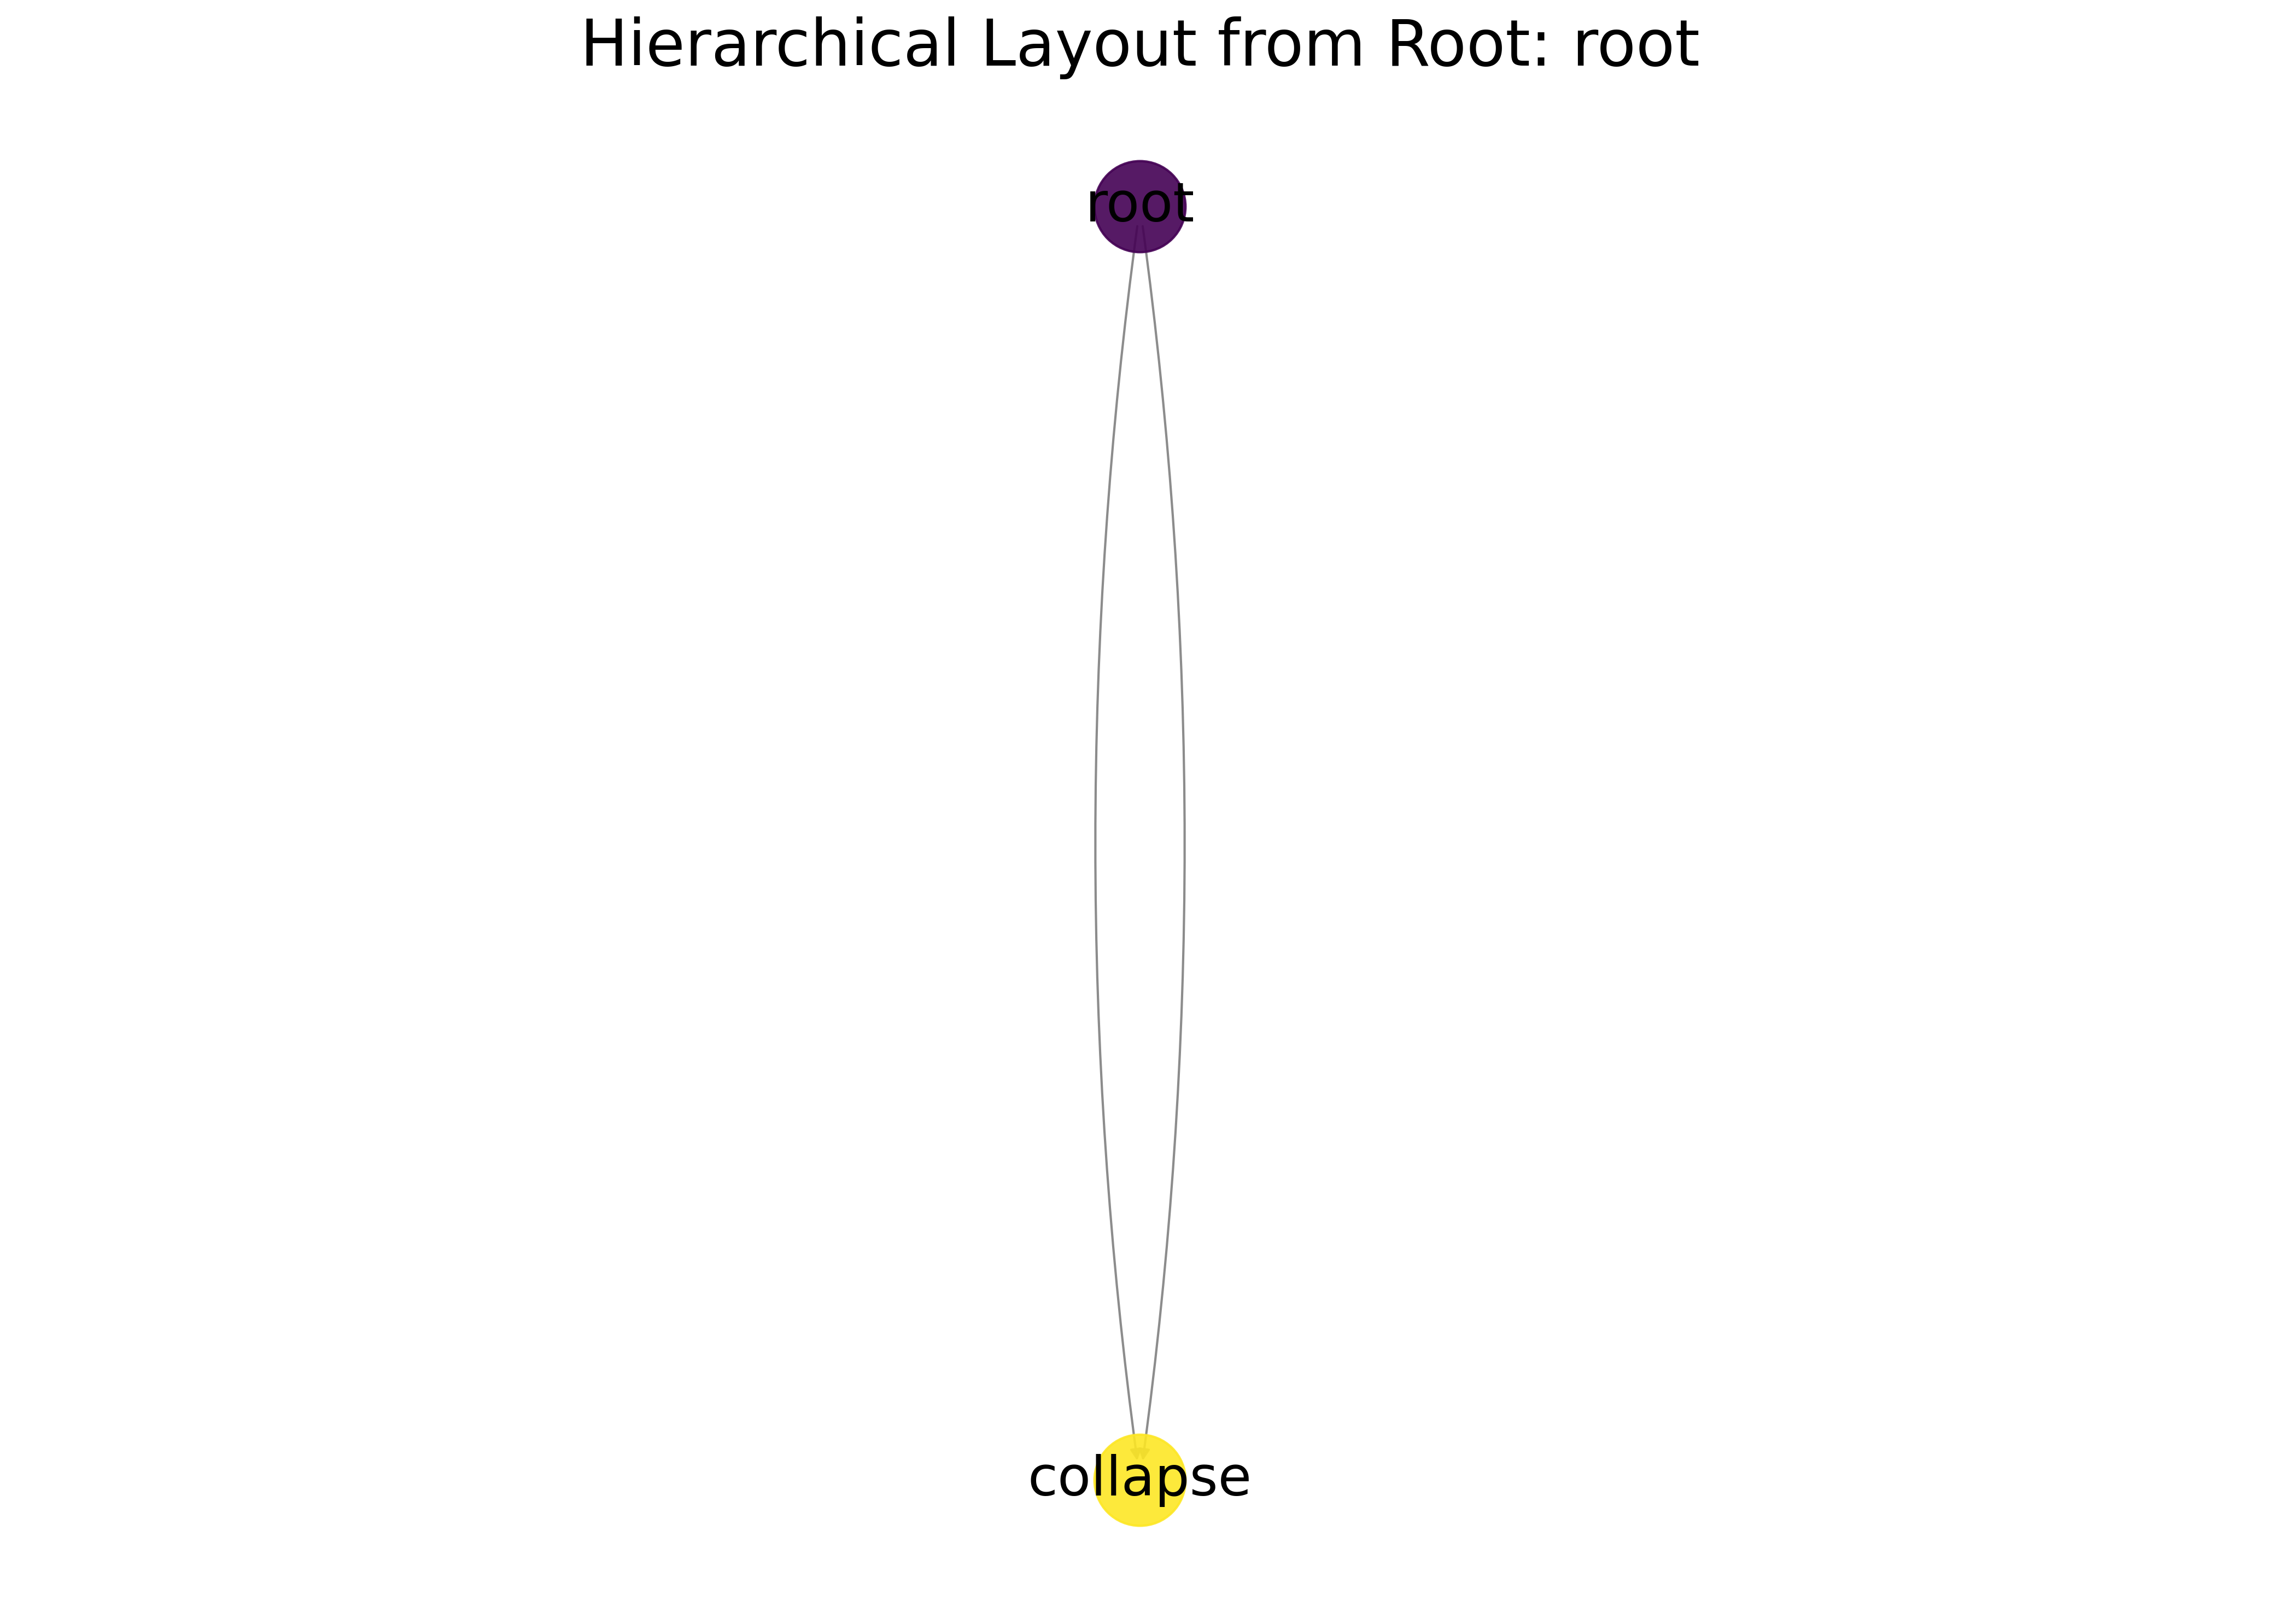
\includegraphics[width=\linewidth, height=0.18\textheight, keepaspectratio]{images/ExternalBaselines/best_F_ma_collapse_prod.png}

  {\small\textbf{(b)} F\_ma (Yes)}
\end{minipage}

\vspace{0.5em} % 减小间距以节省空间

% --- Row 2 ---
\begin{minipage}{0.48\linewidth}
  \centering
  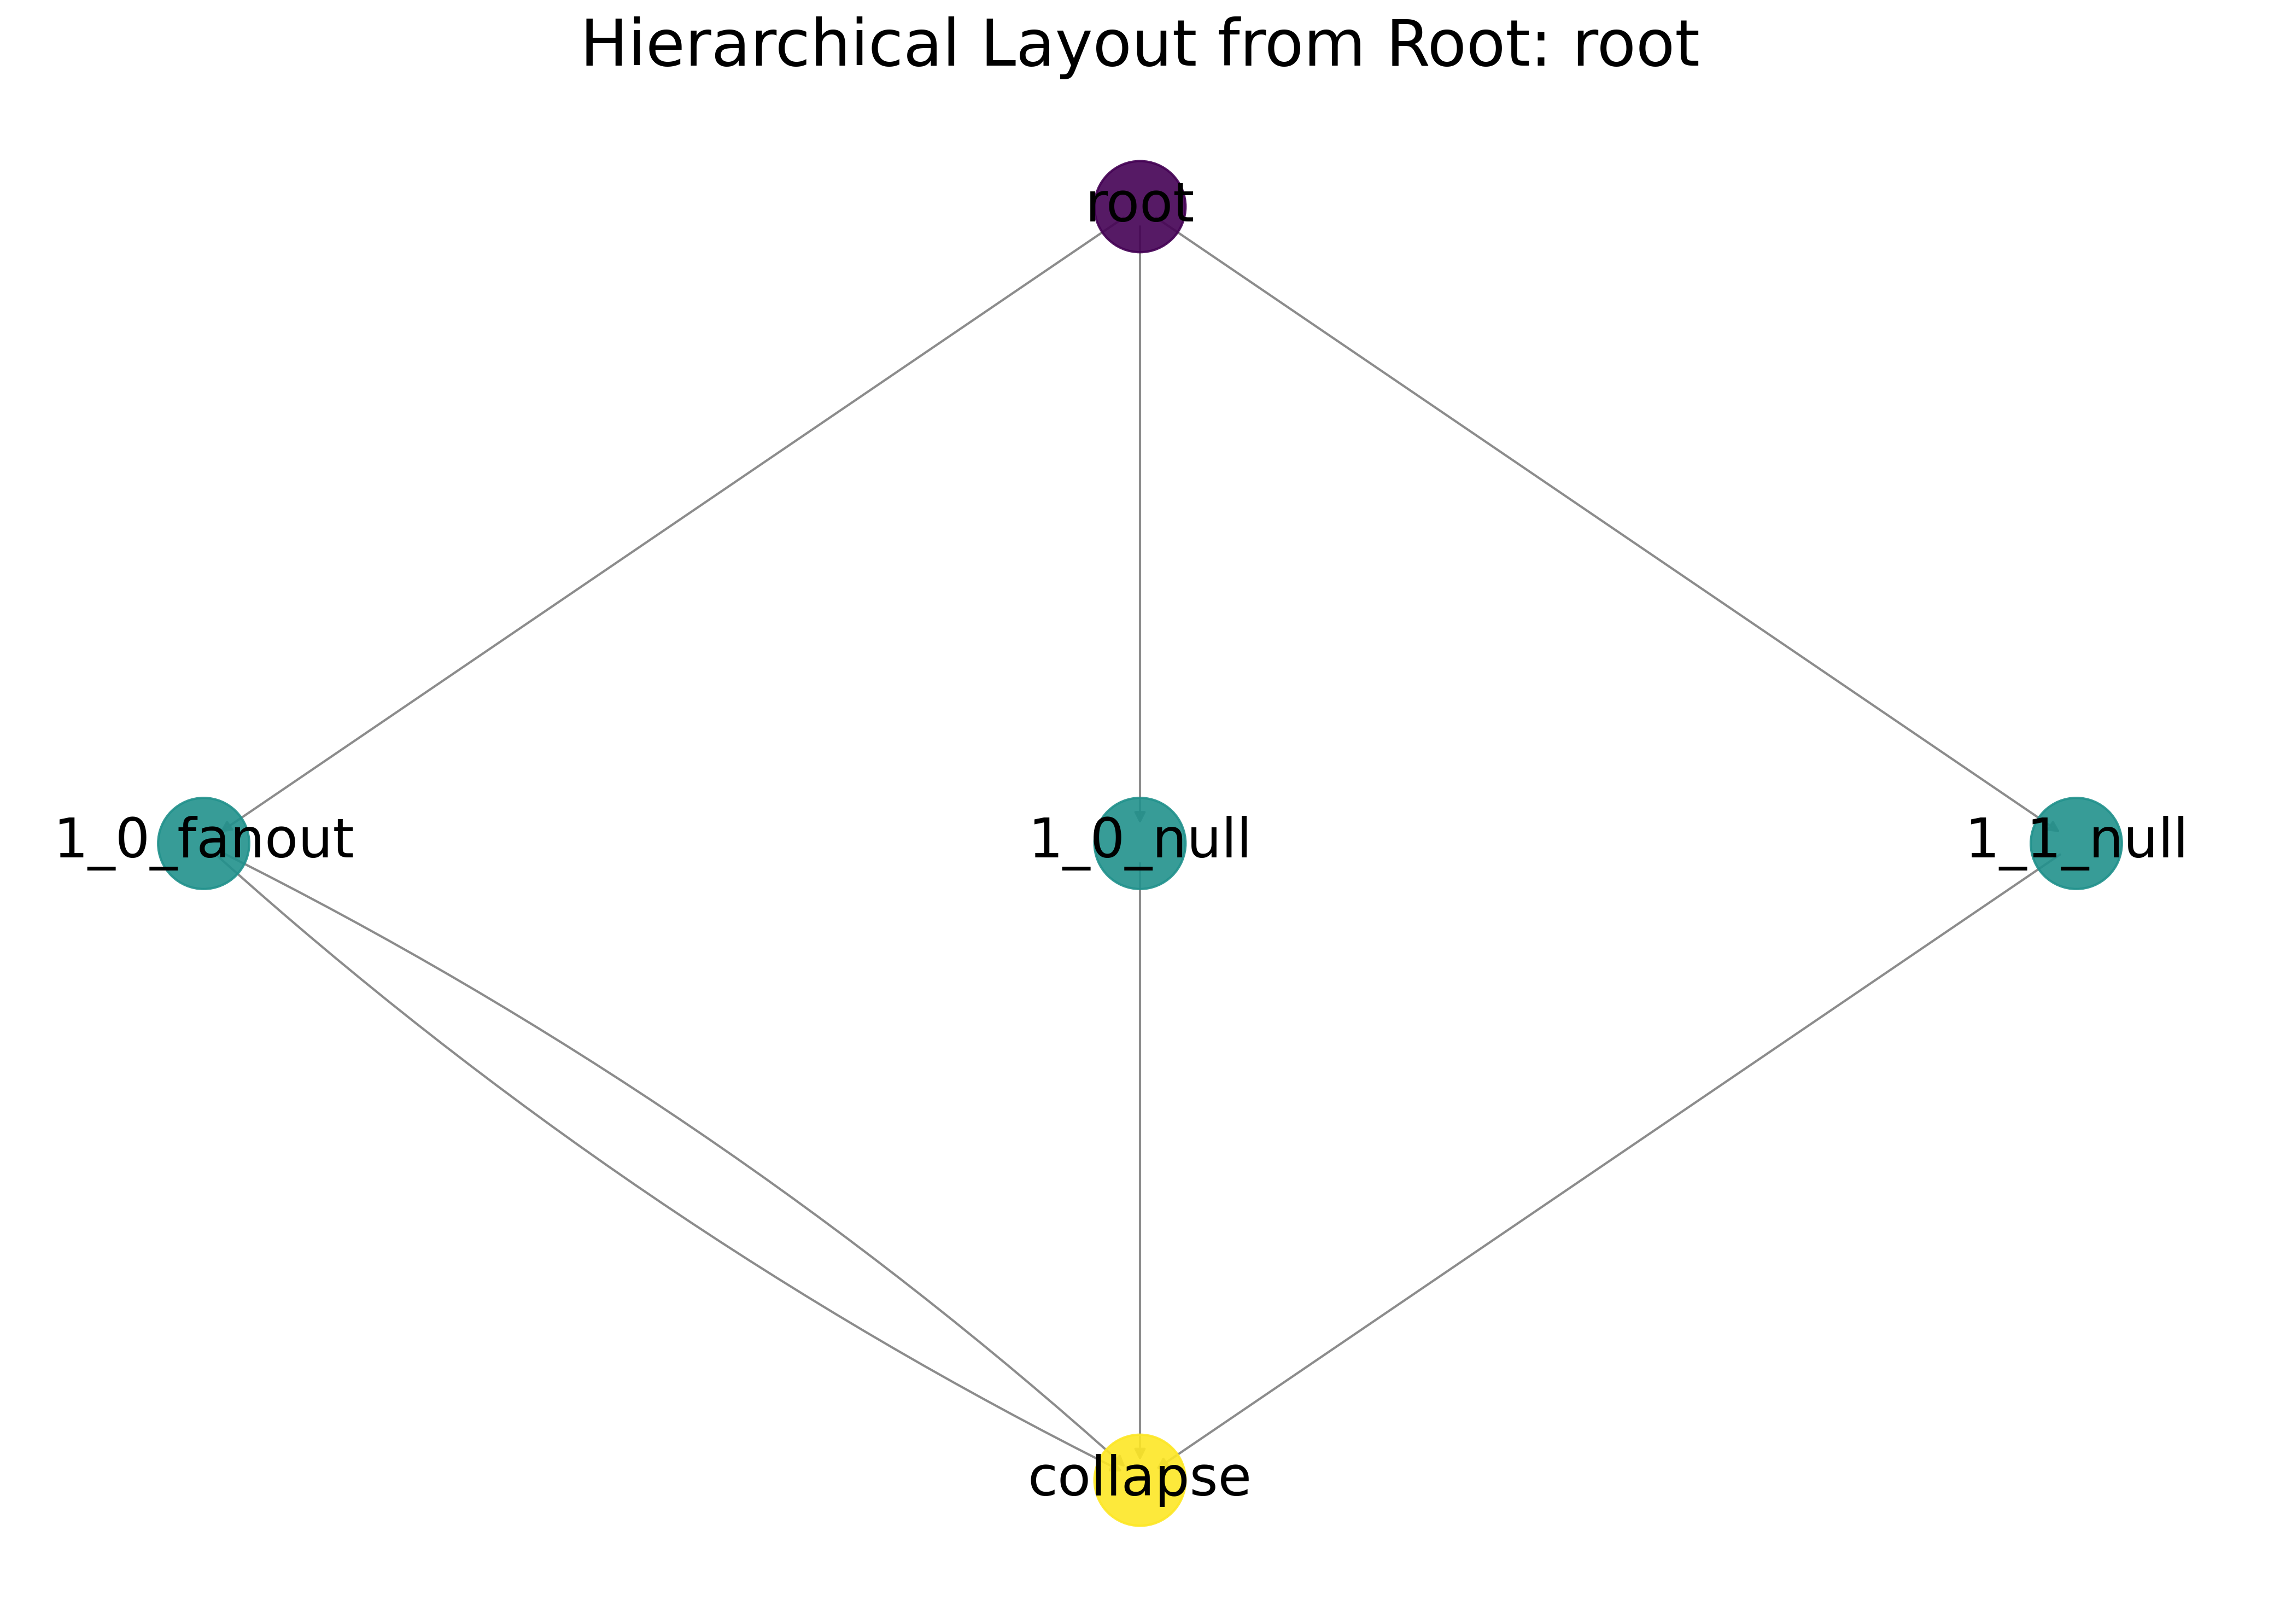
\includegraphics[width=\linewidth, height=0.18\textheight, keepaspectratio]{images/ExternalBaselines/best_KE_collapse_prod.png}

  {\small\textbf{(c)} KE (Yes)}
\end{minipage}
\hfill
\begin{minipage}{0.48\linewidth}
  \centering
  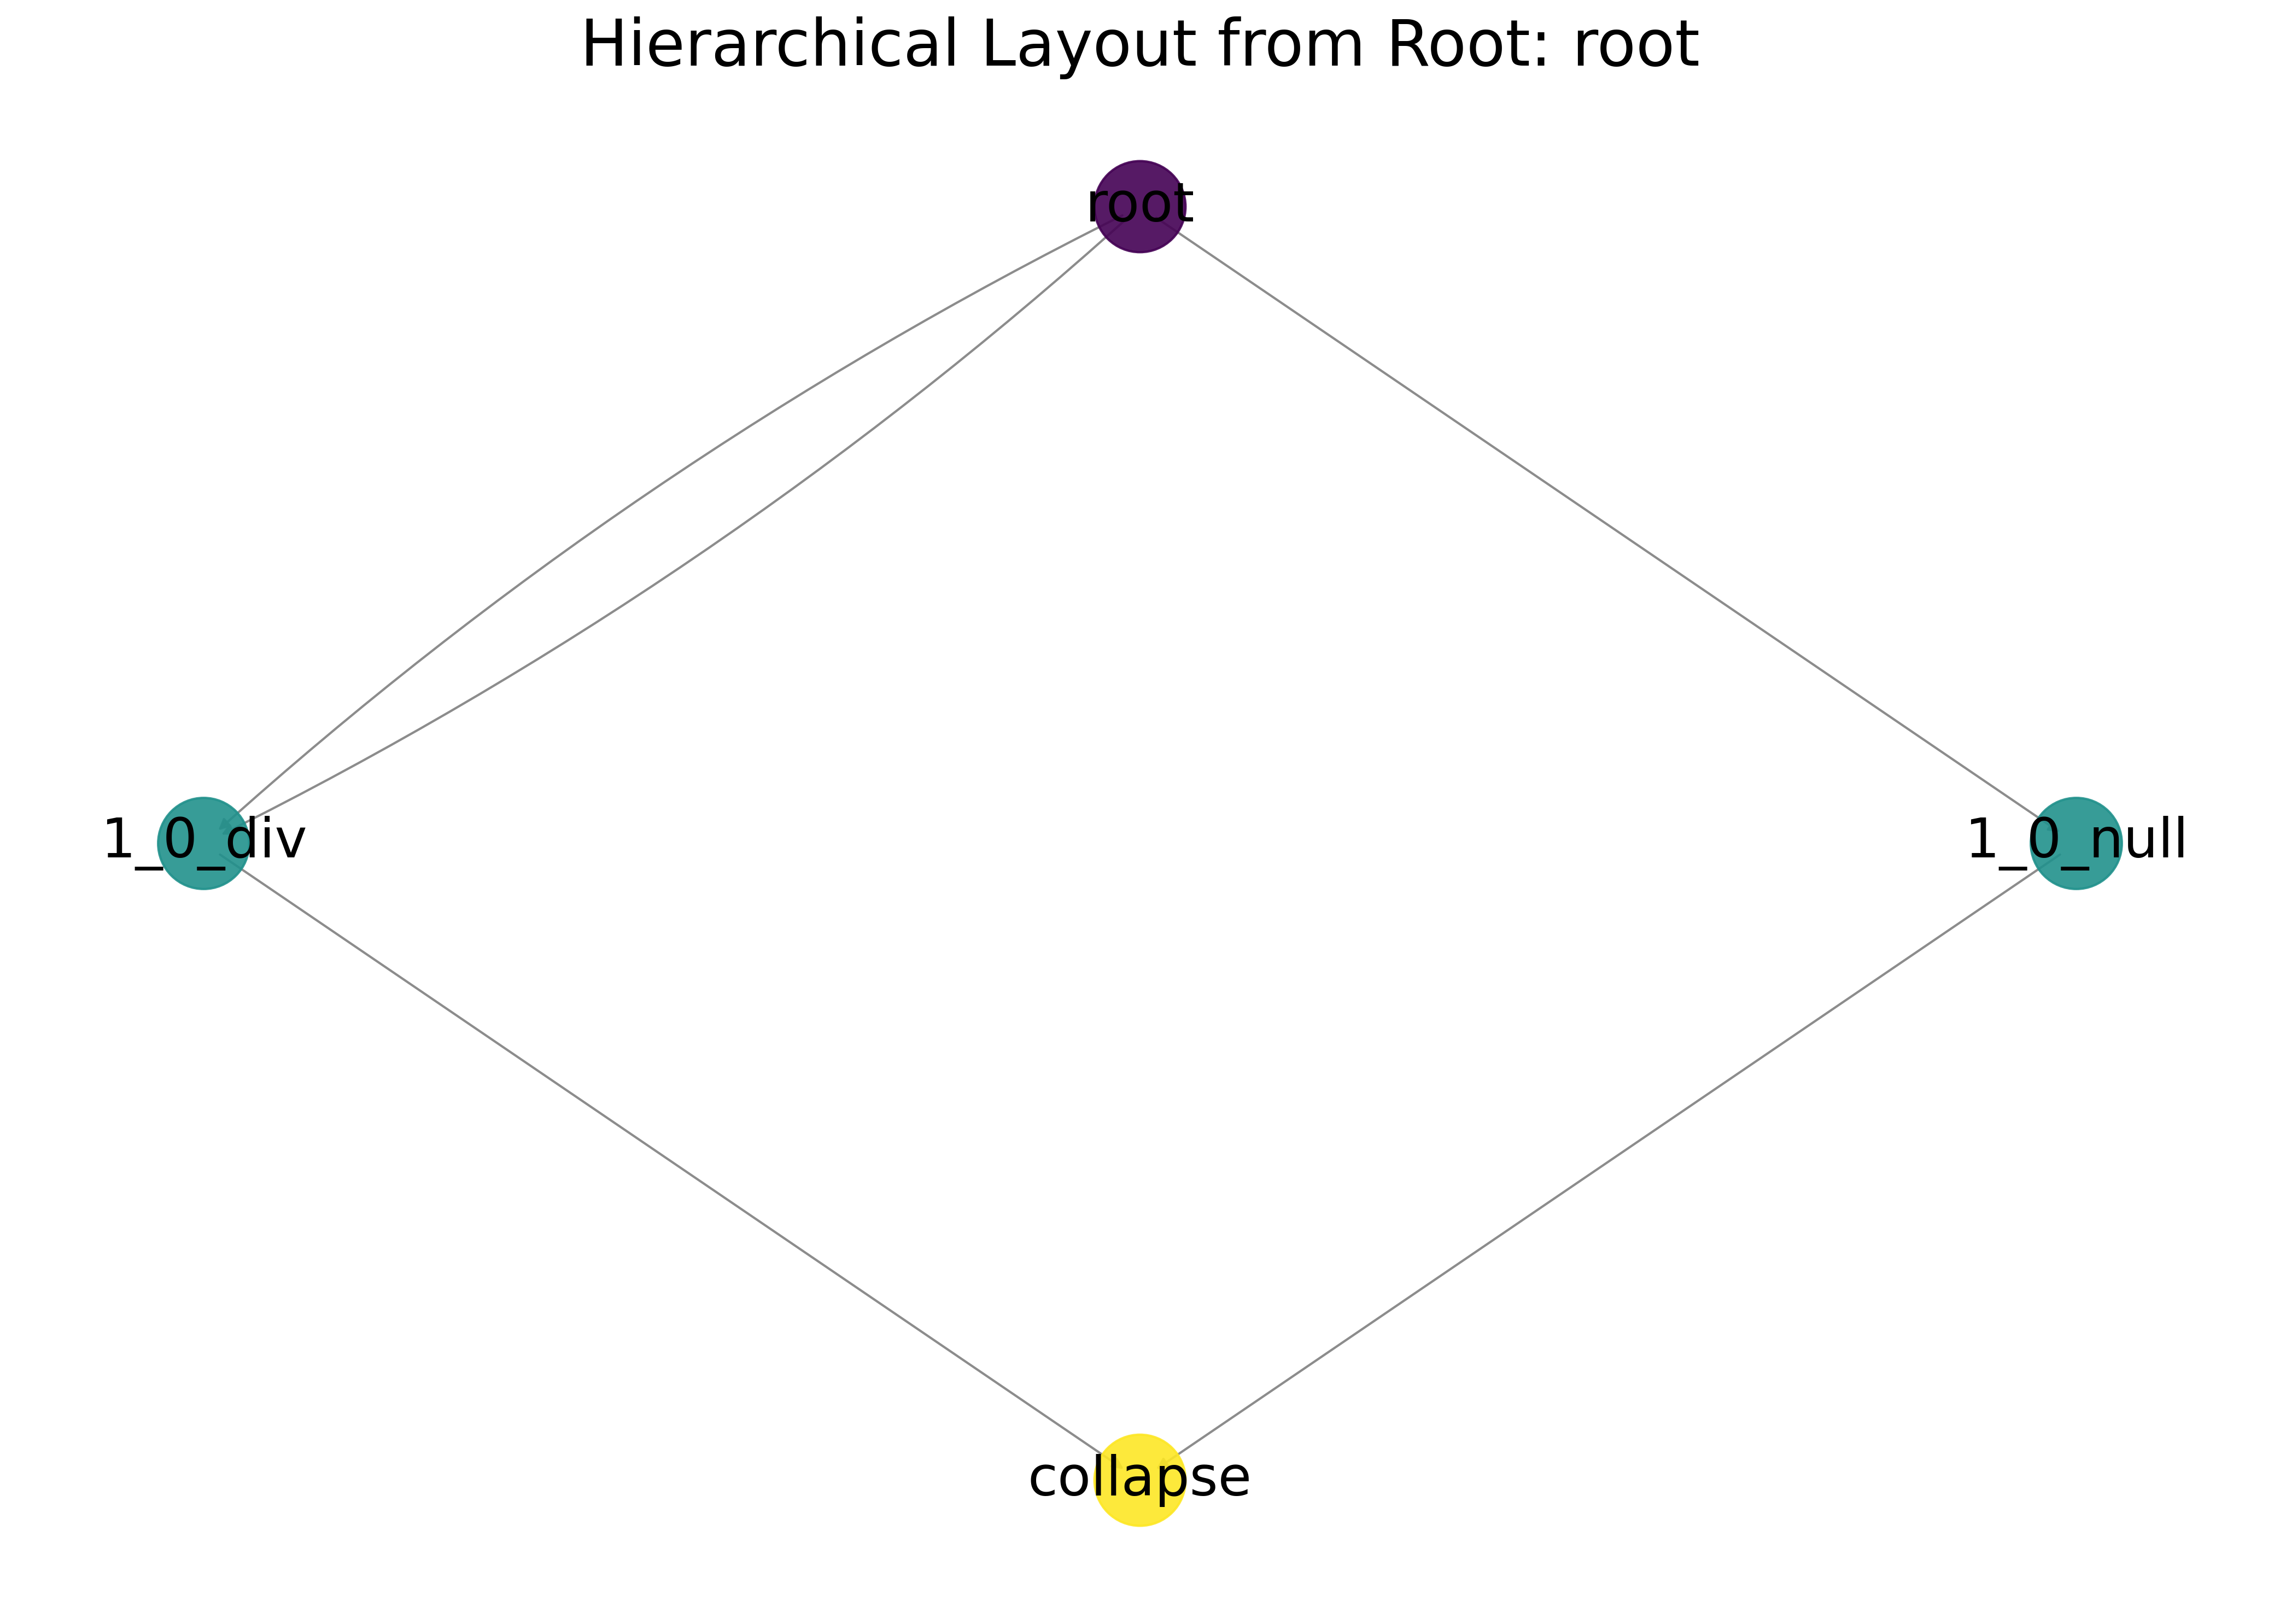
\includegraphics[width=\linewidth, height=0.18\textheight, keepaspectratio]{images/ExternalBaselines/best_Coulomb_collapse_prod.png}

  {\small\textbf{(d)} Coulomb (No)}
\end{minipage}

\vspace{0.5em}

% --- Row 3 ---
\begin{minipage}{0.48\linewidth}
  \centering
  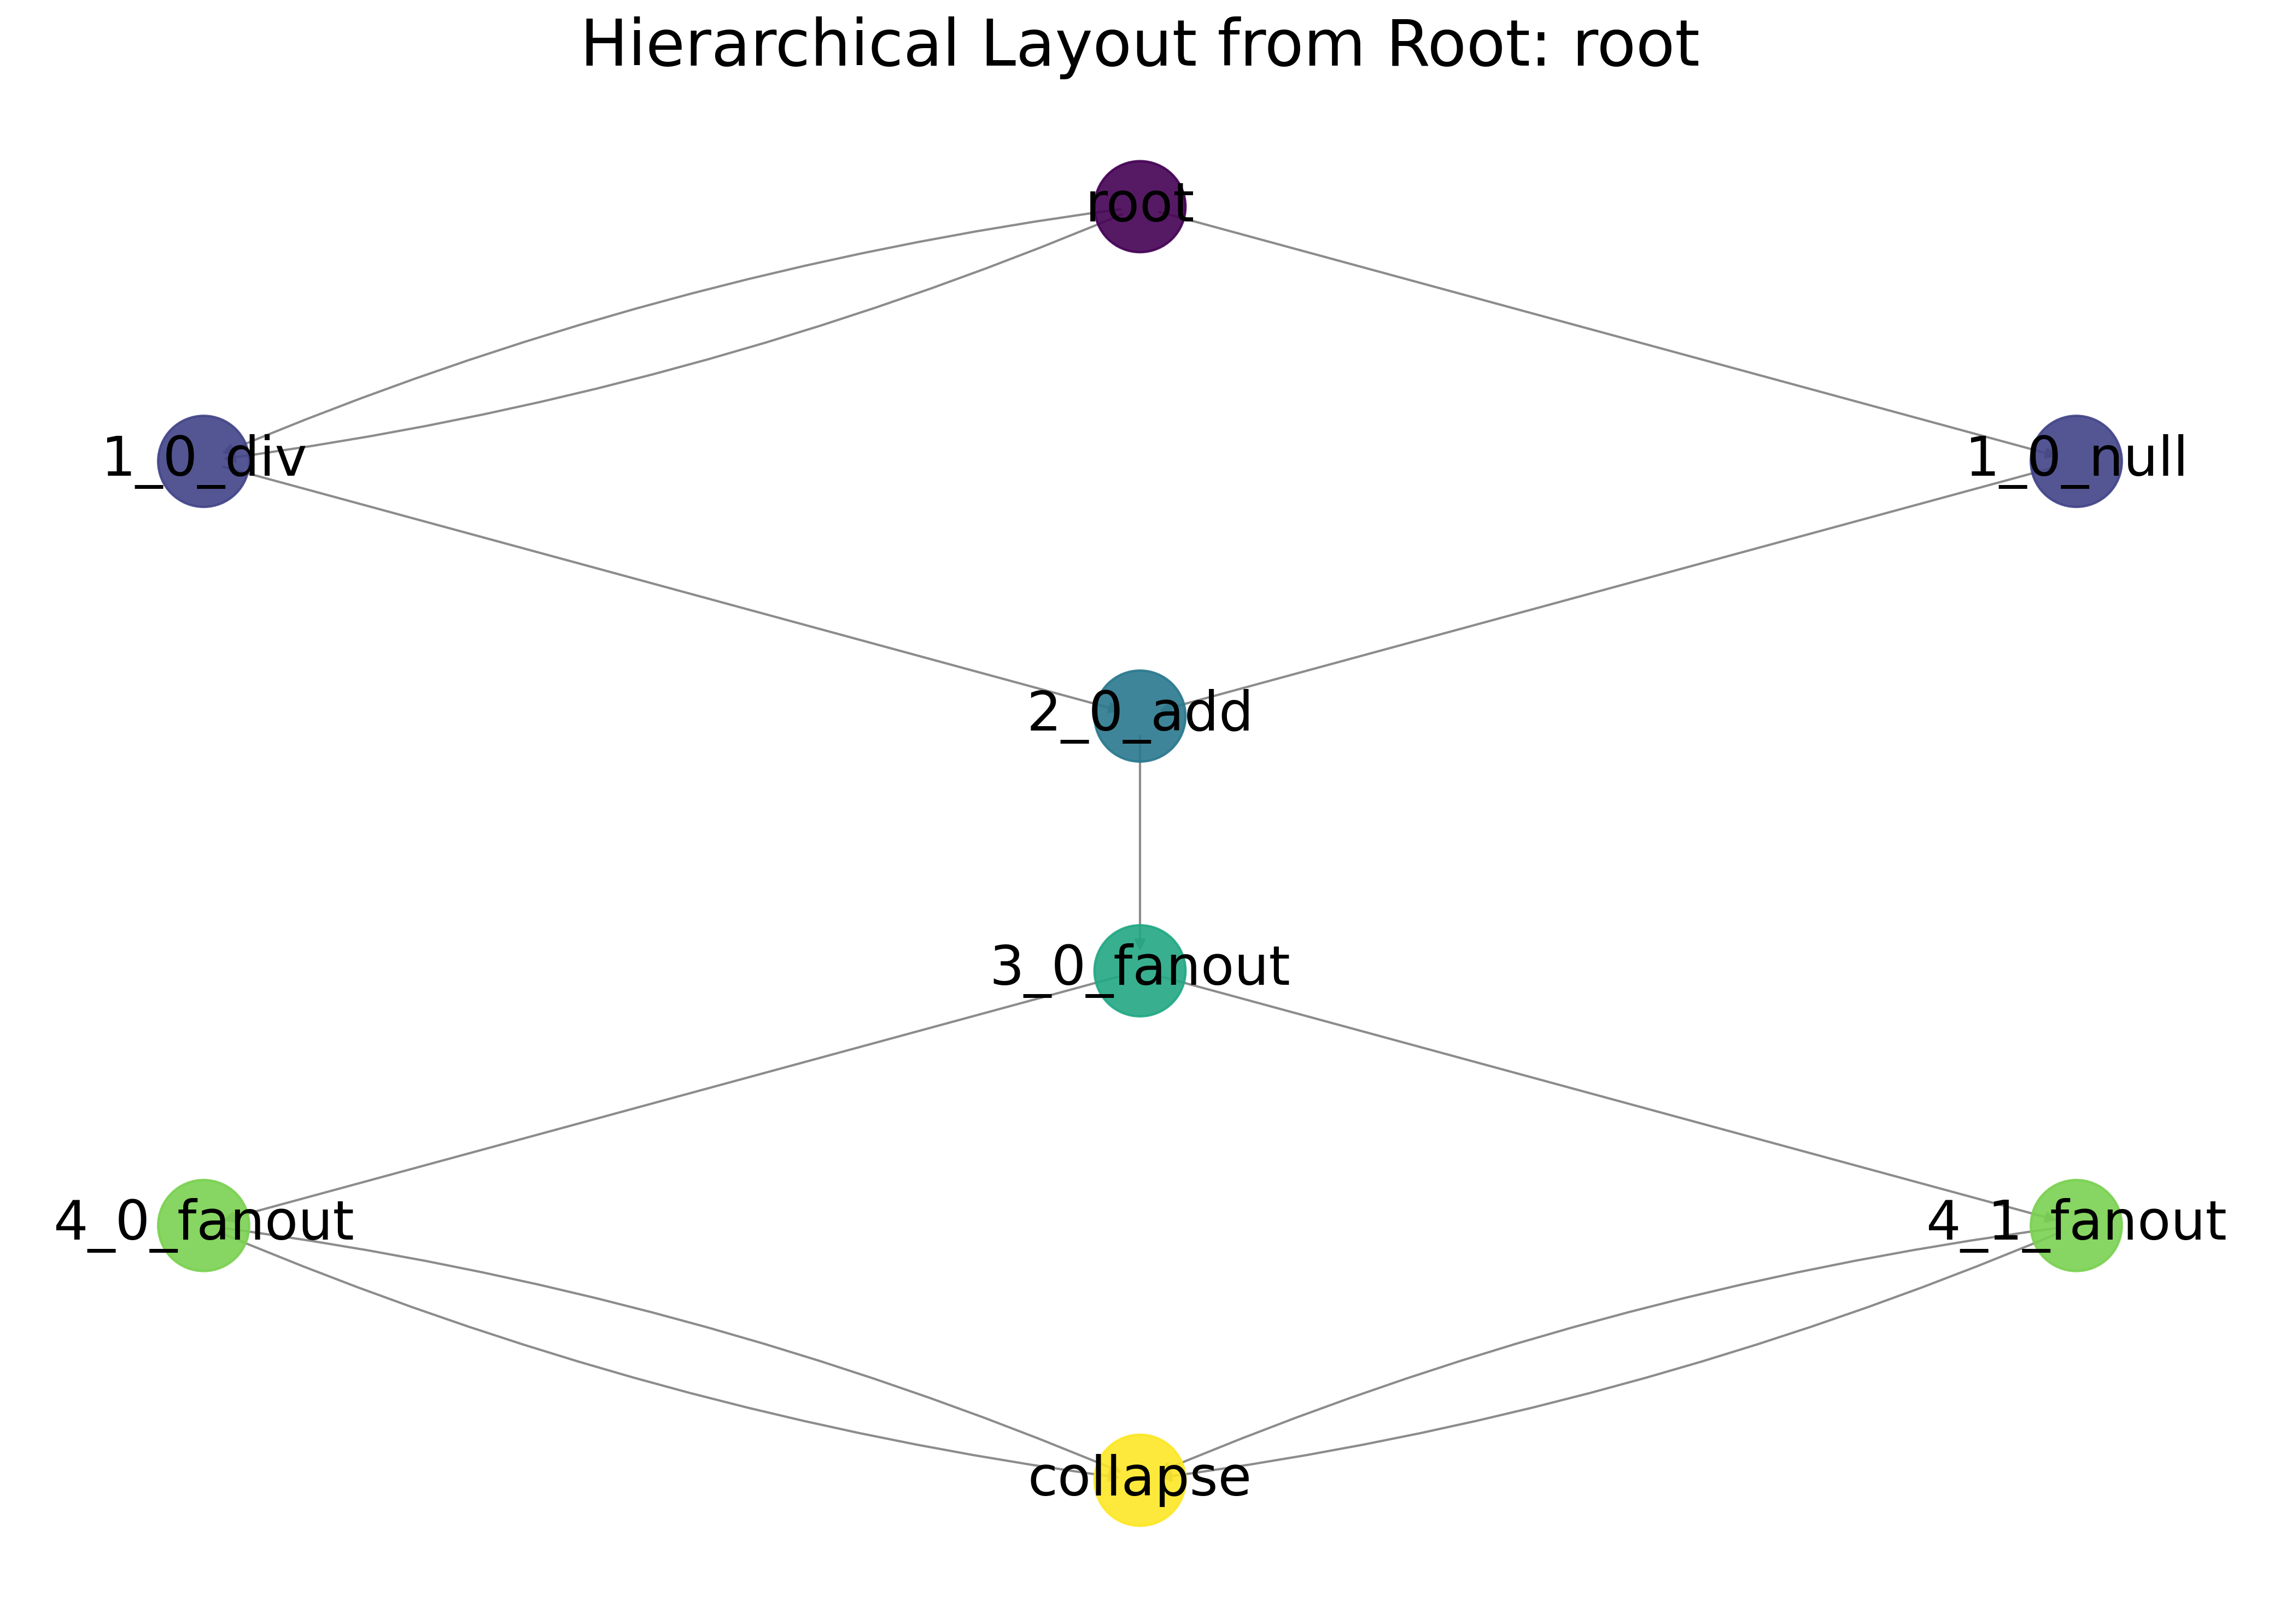
\includegraphics[width=\linewidth, height=0.18\textheight, keepaspectratio]{images/ExternalBaselines/best_IdealGas_collapse_prod.png}

  {\small\textbf{(e)} Ideal Gas (No)}
\end{minipage}
\hfill
\begin{minipage}{0.48\linewidth}
  \centering
  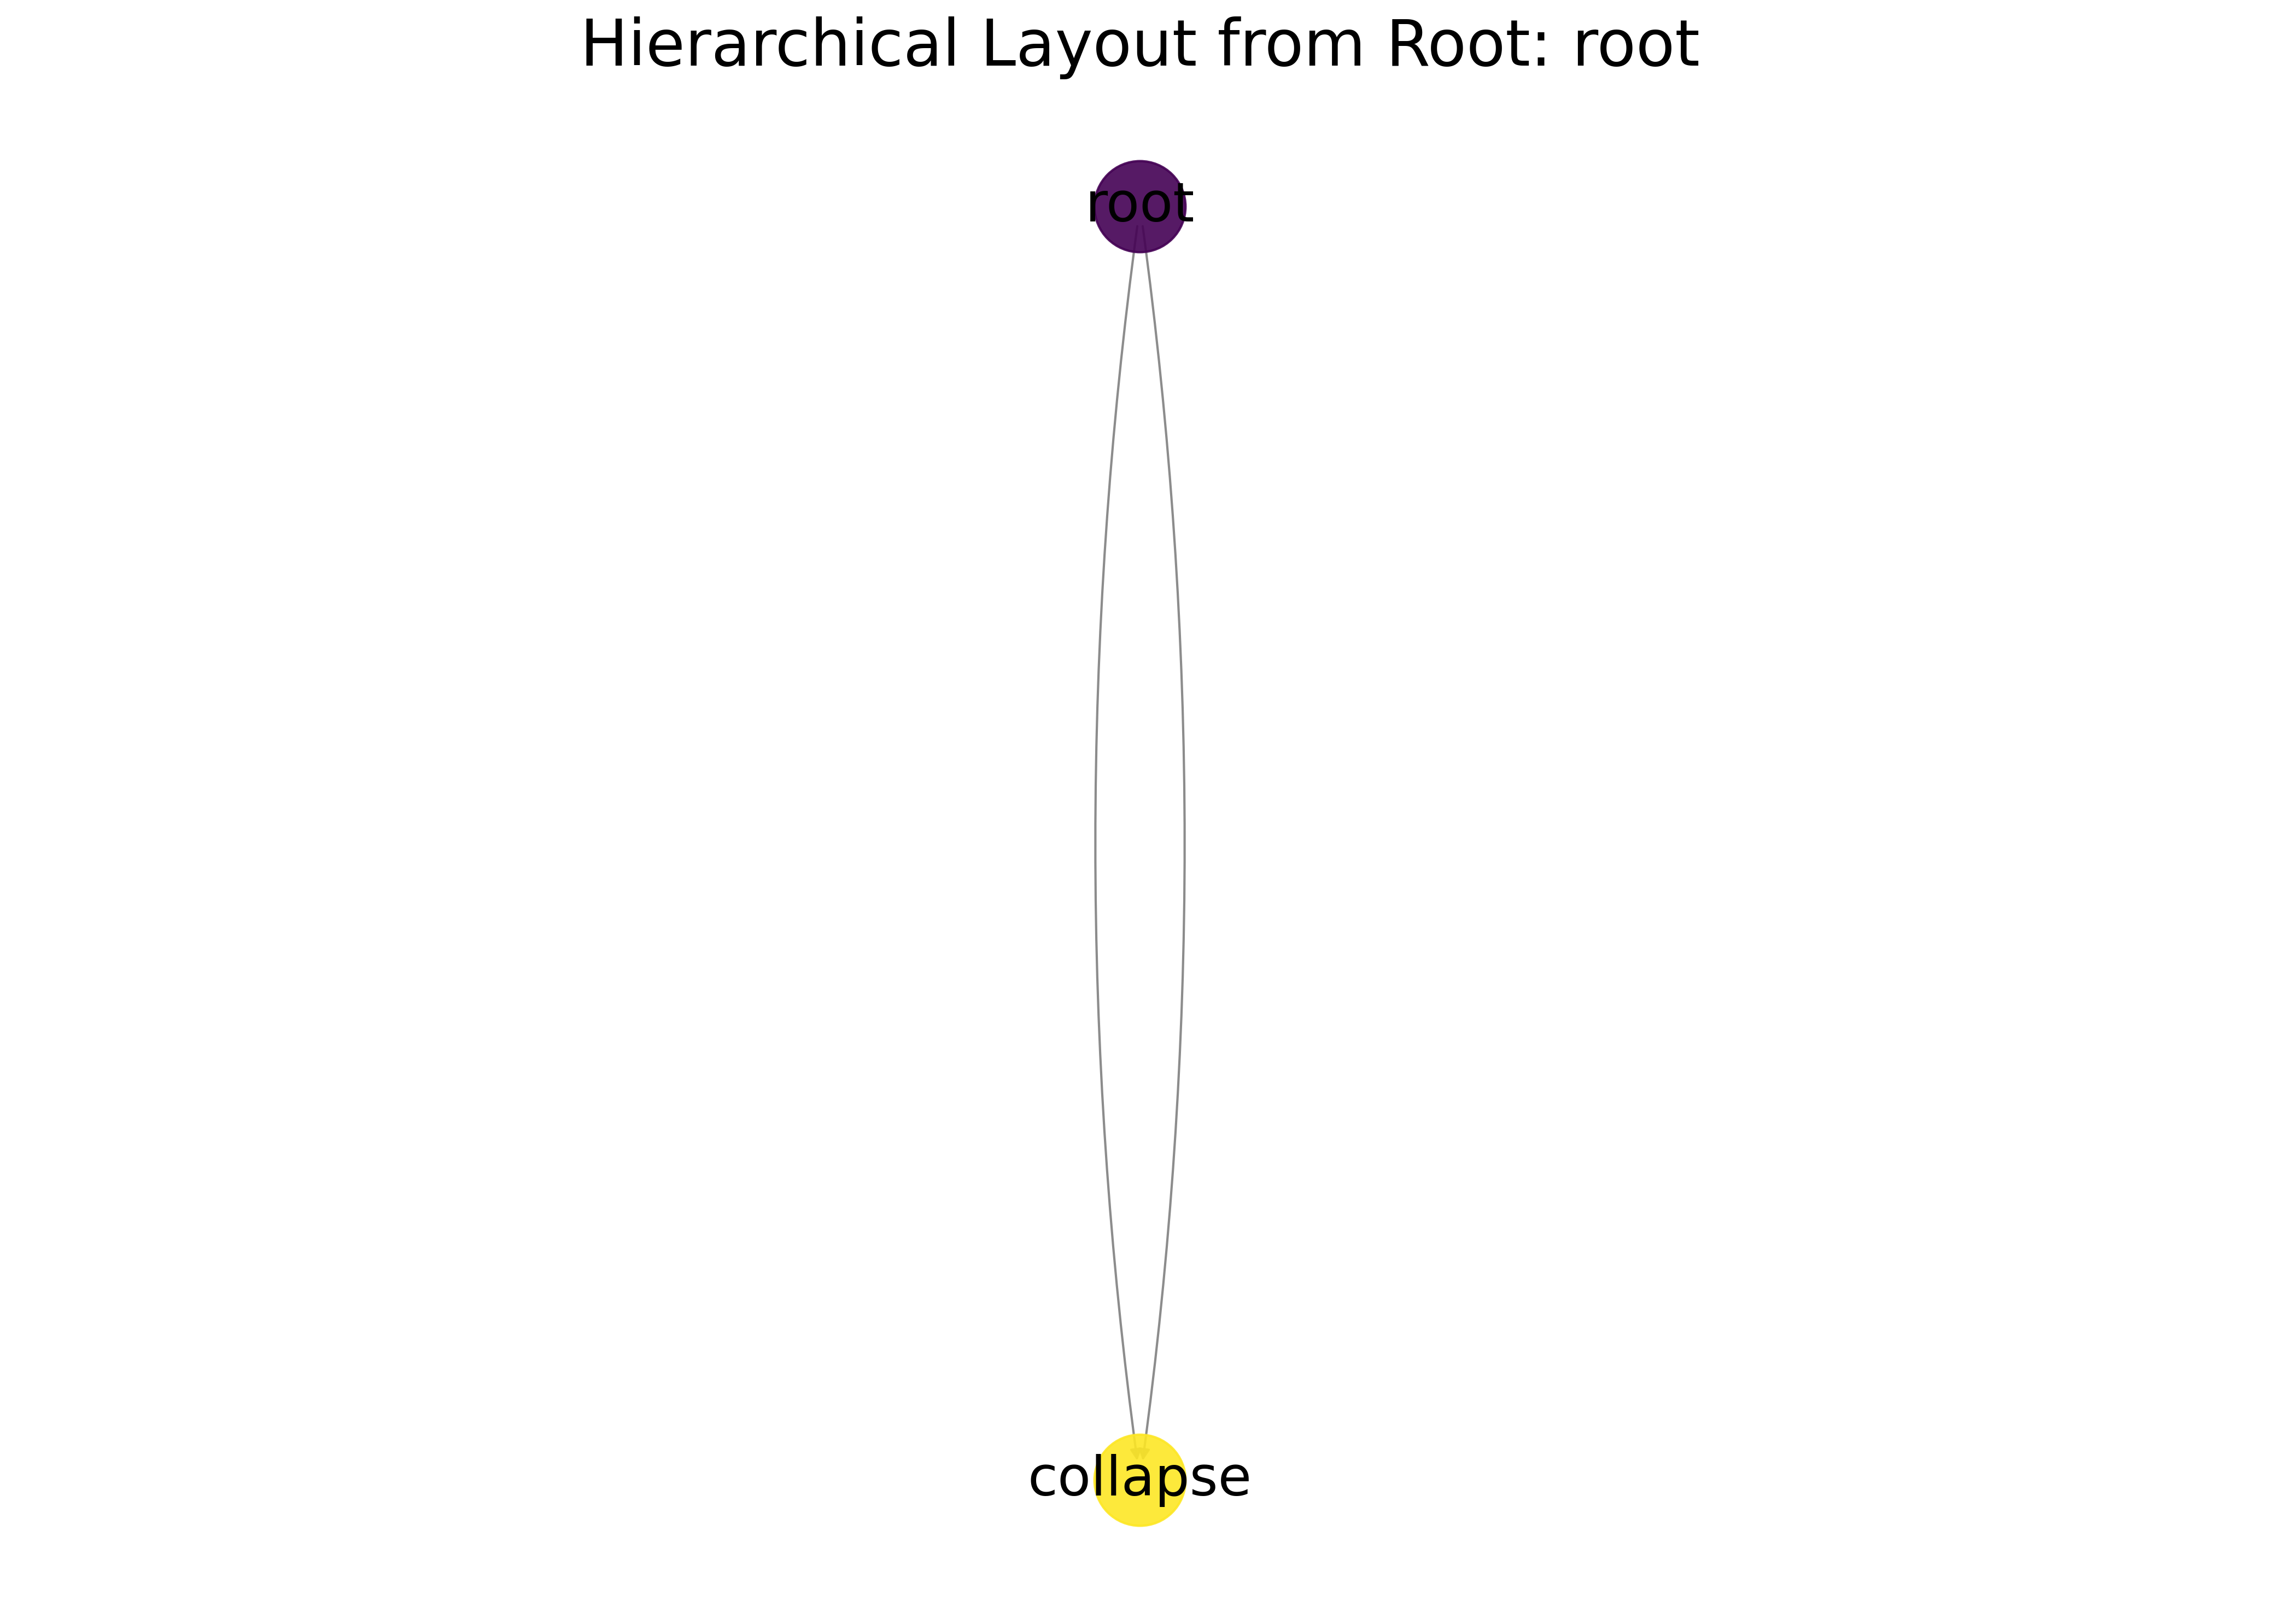
\includegraphics[width=\linewidth, height=0.18\textheight, keepaspectratio]{images/ExternalBaselines/best_OhmsLaw_collapse_prod.png}

  {\small\textbf{(f)} Ohm's Law (Yes)}
\end{minipage}

\vspace{0.5em}

% --- Row 4 ---
\begin{minipage}{0.48\linewidth}
  \centering
  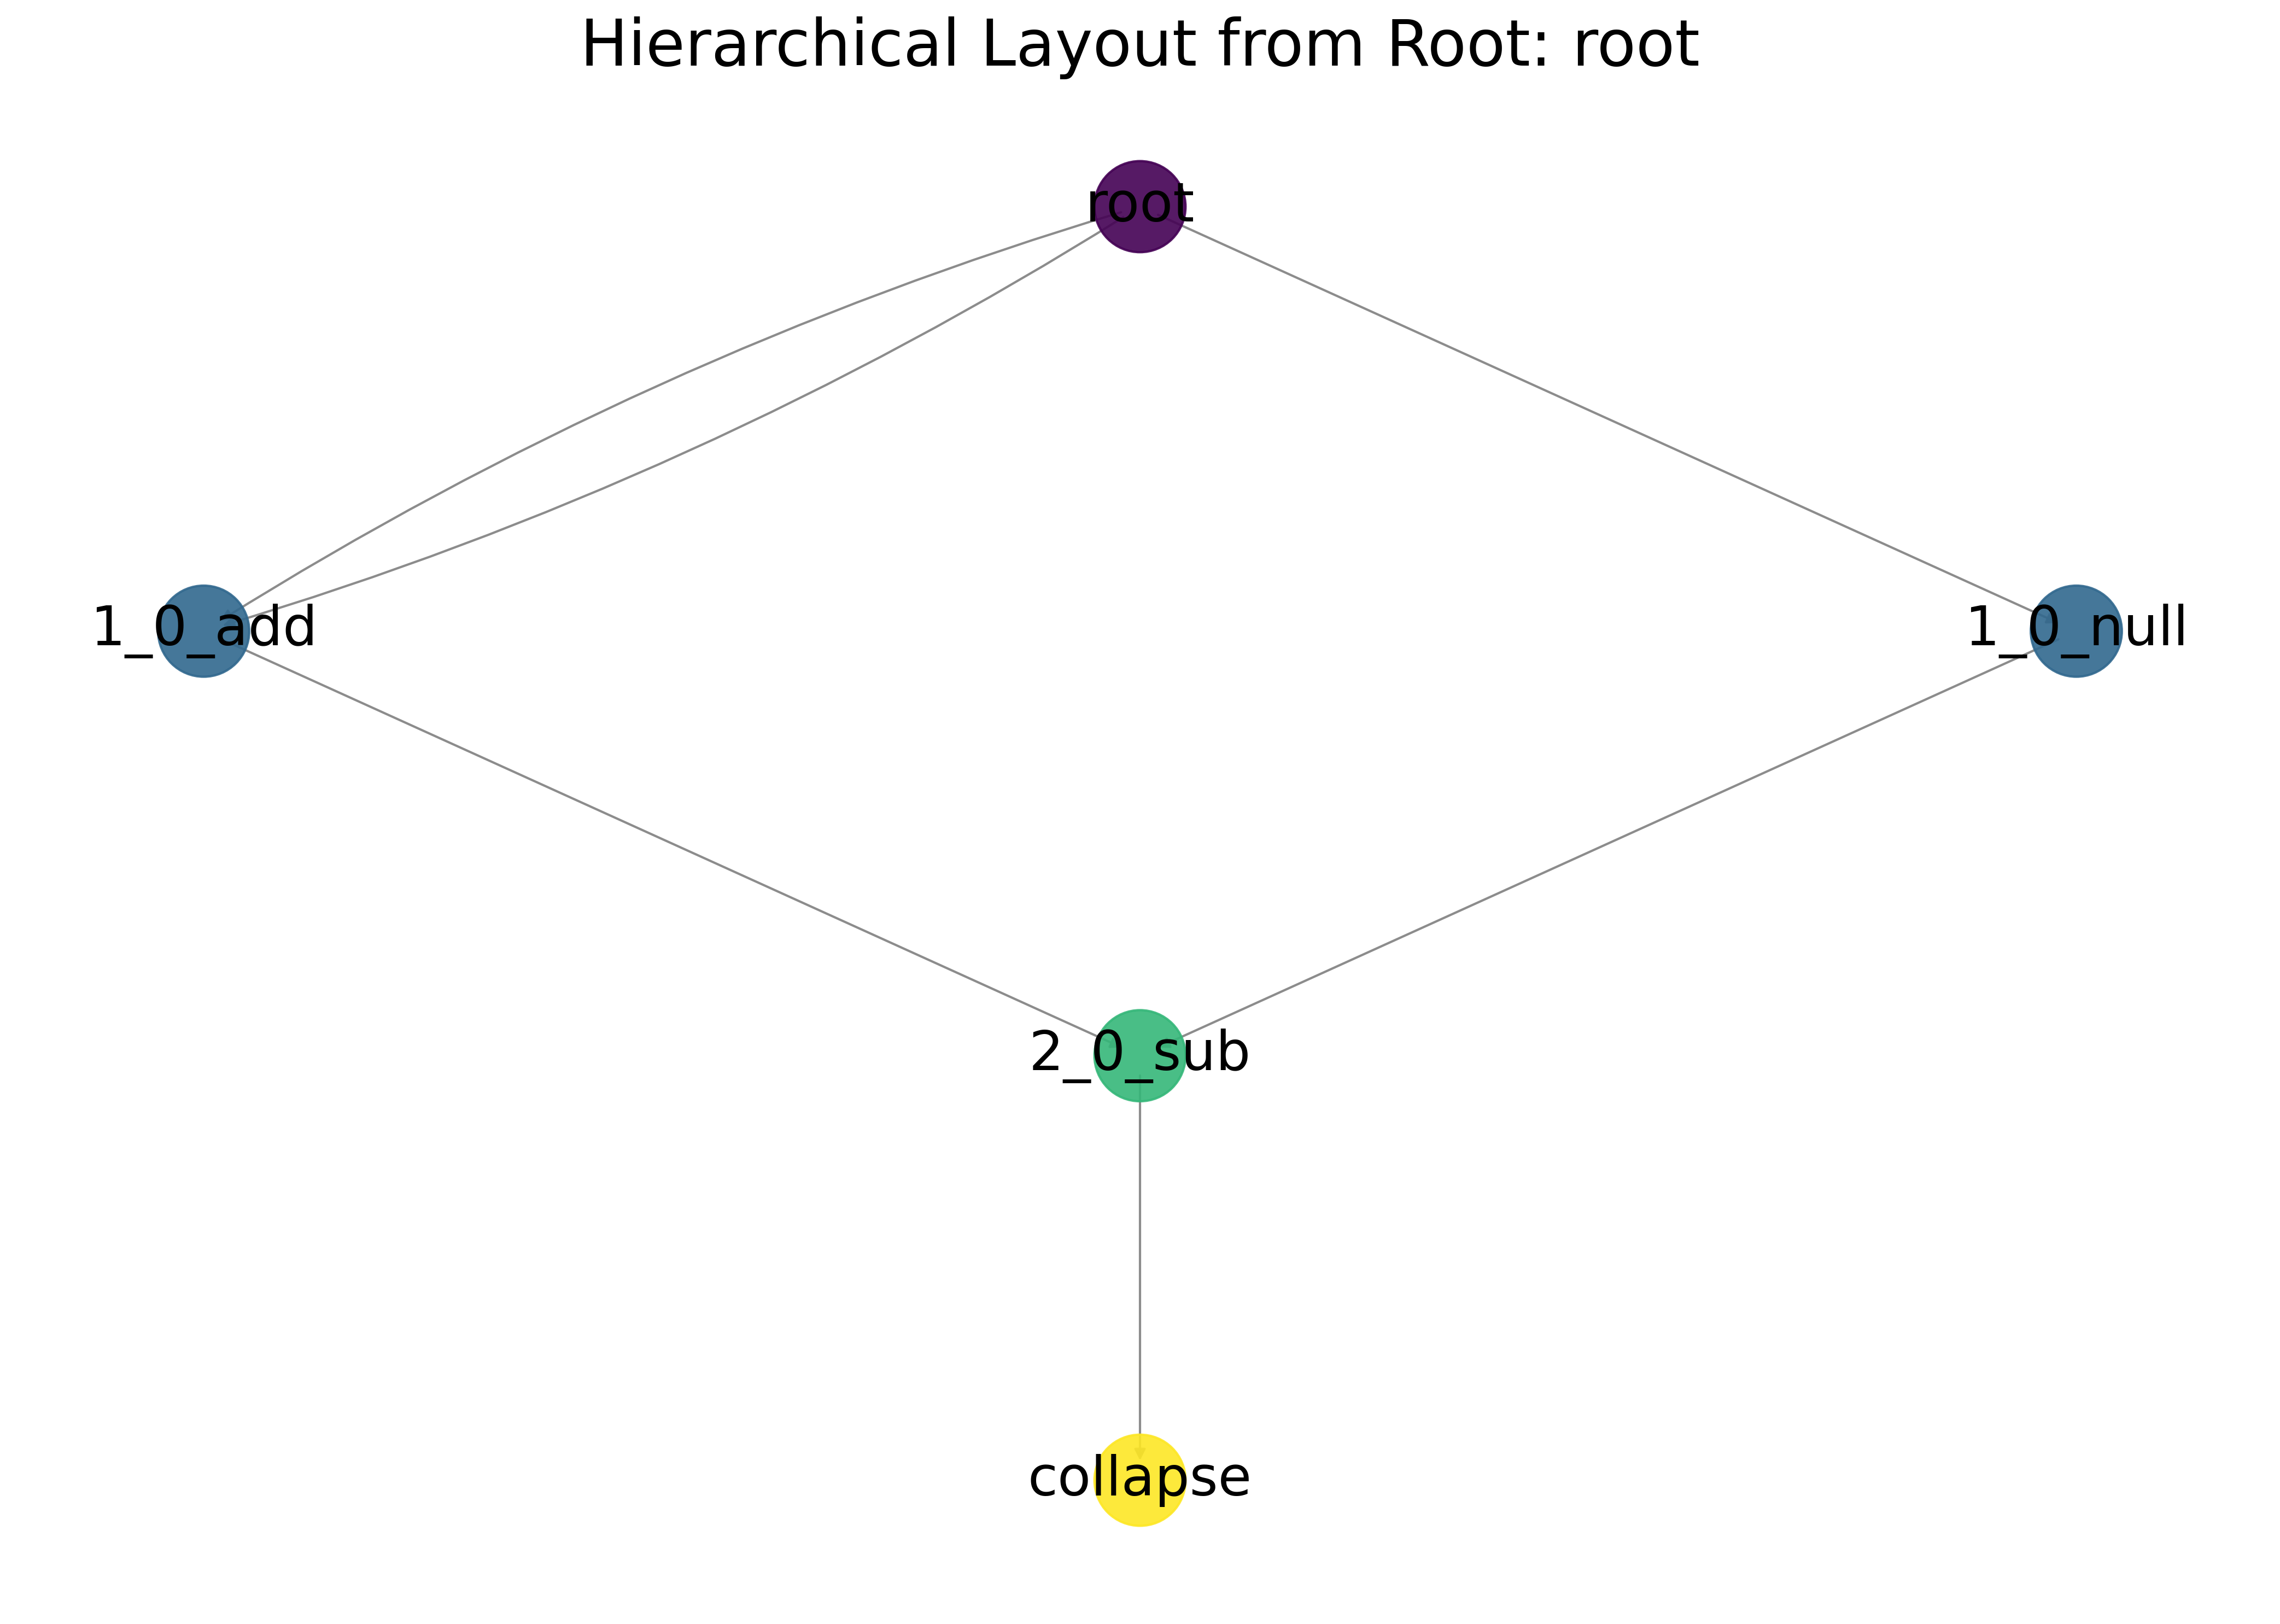
\includegraphics[width=\linewidth, height=0.18\textheight, keepaspectratio]{images/ExternalBaselines/best_Acceleration_collapse_prod.png}

  {\small\textbf{(g)} Acceleration (No)}
\end{minipage}
\hfill
\begin{minipage}{0.48\linewidth}
  \centering
  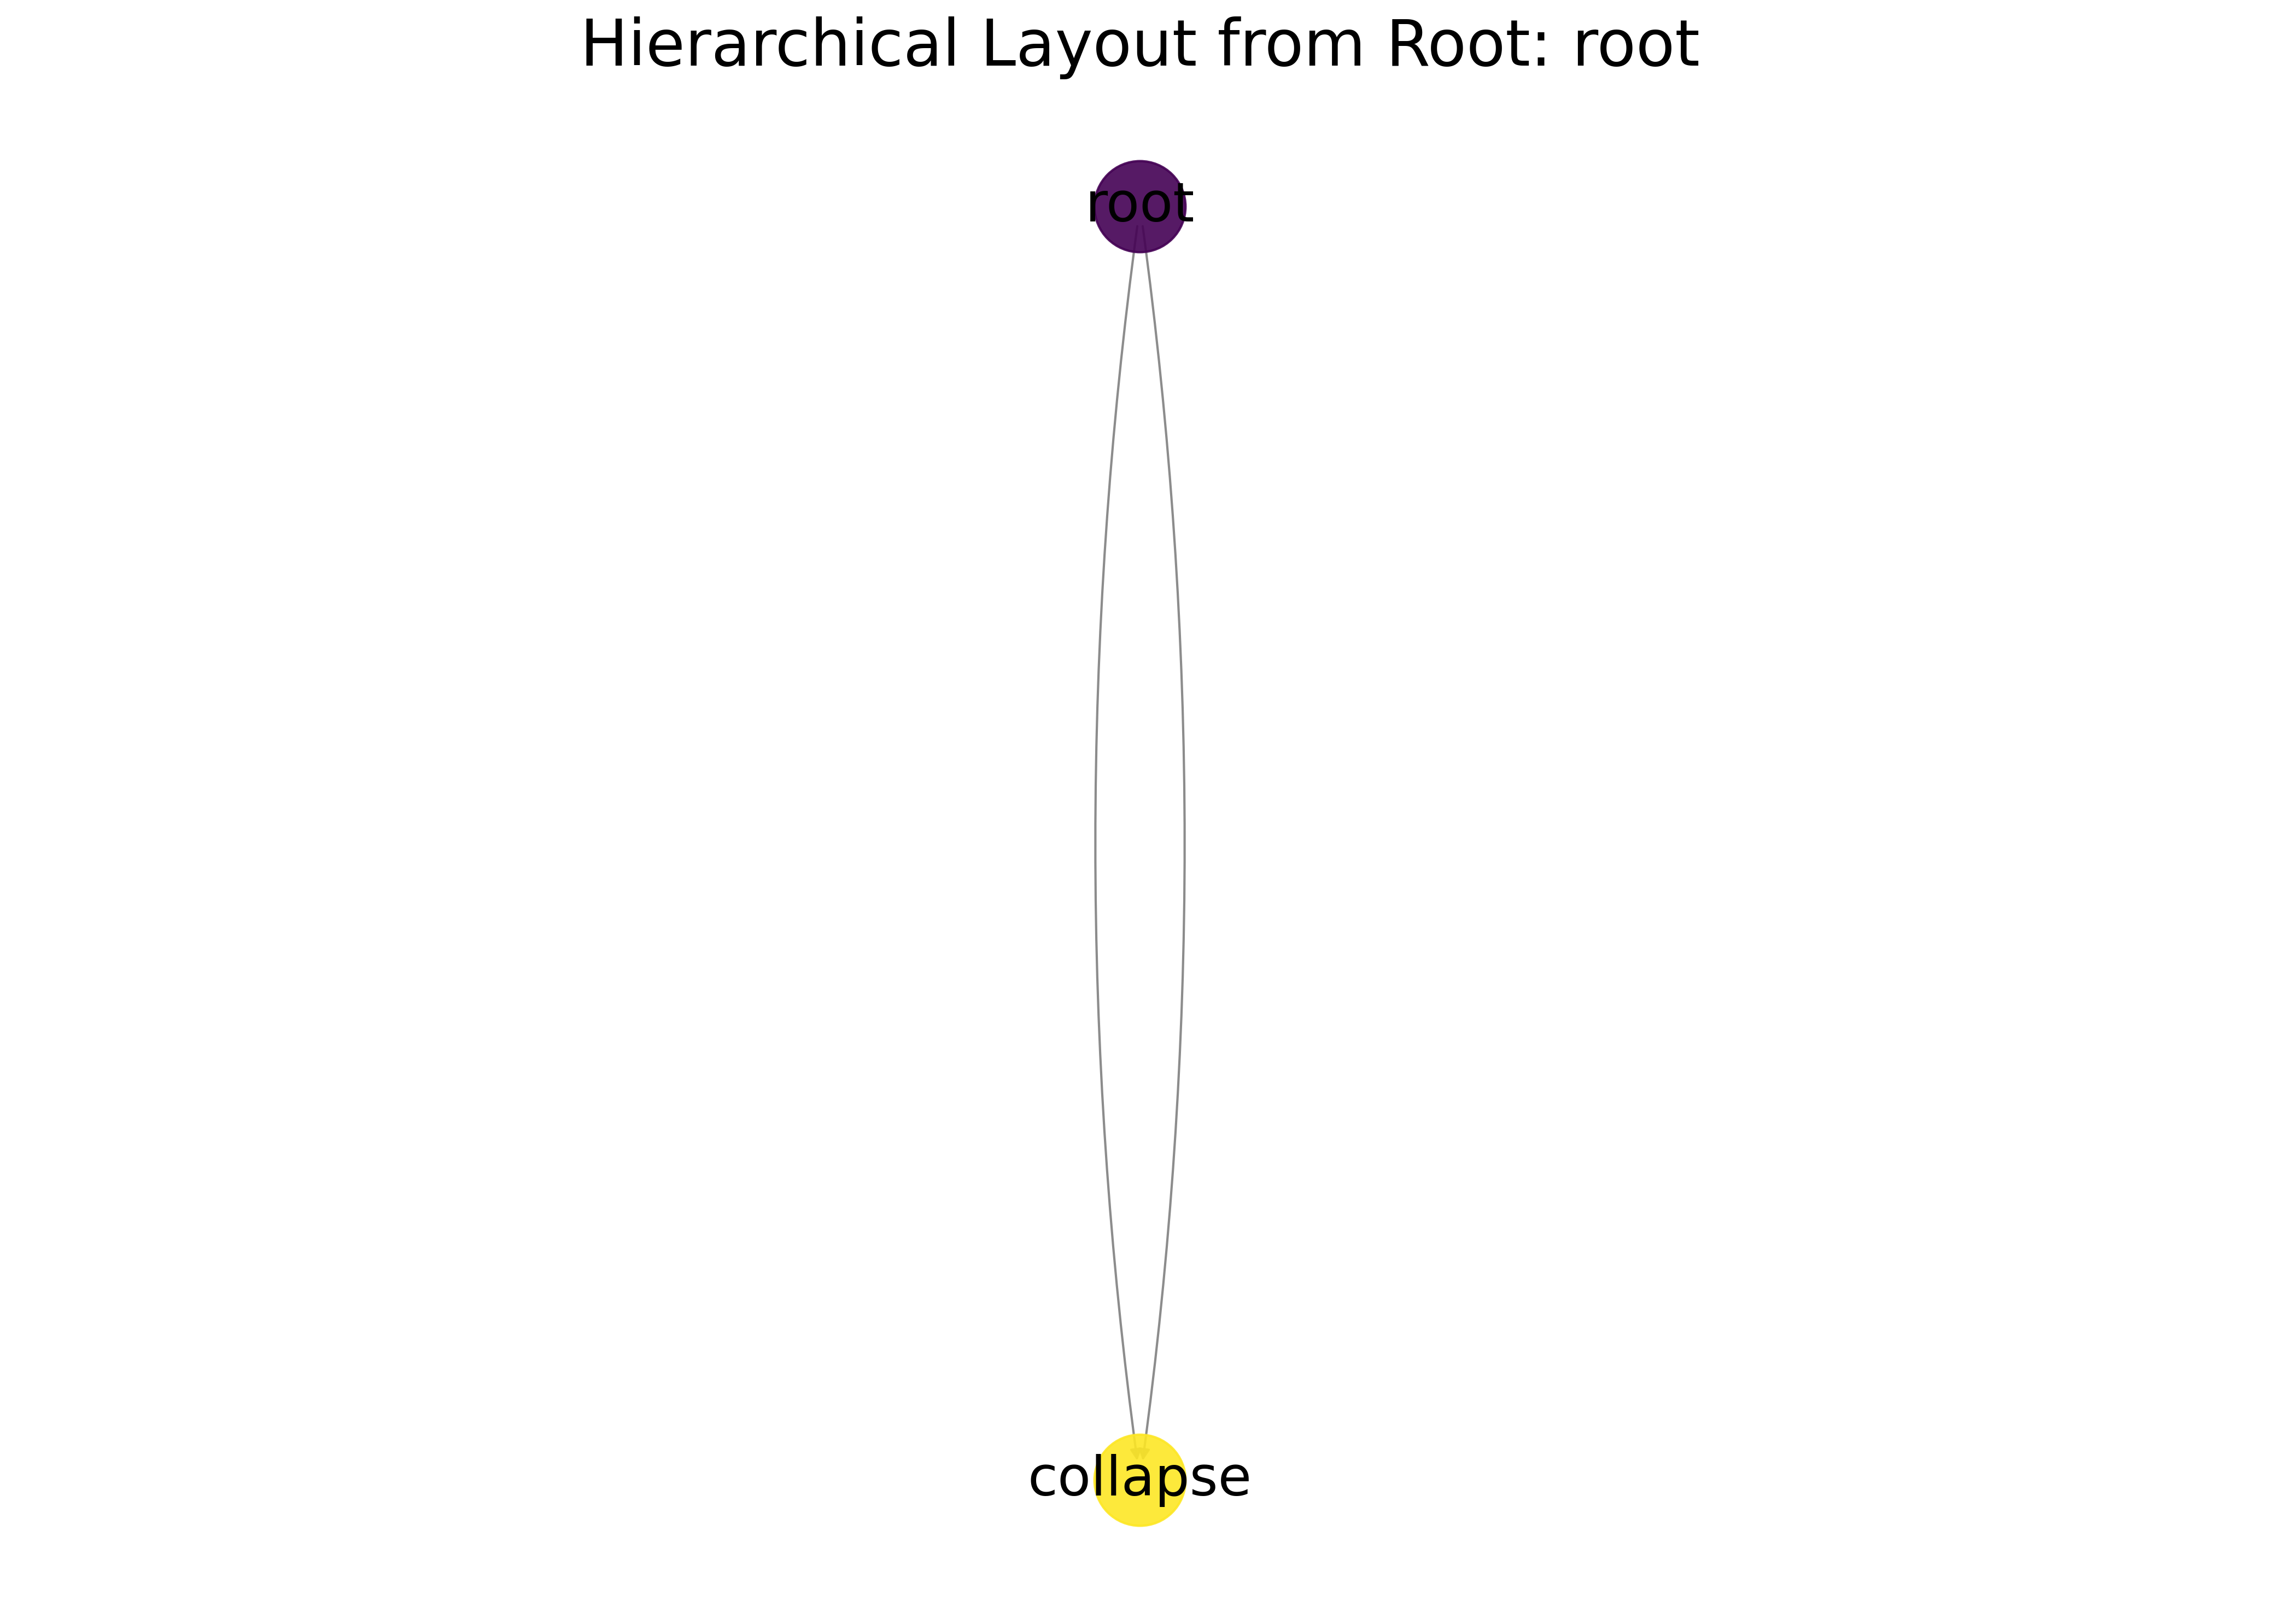
\includegraphics[width=\linewidth, height=0.18\textheight, keepaspectratio]{images/ExternalBaselines/best_Power_collapse_prod.png}

  {\small\textbf{(h)} Power (Yes)}
\end{minipage}

\end{figure}

\begin{table}[htbp]
\centering
\caption{Symbolic exact match analysis: whether the best expression is 
\textbf{algebraically equivalent} to the ground-truth formula, 
as determined by manual inspection. This is stricter than numerical matching.}
\label{tab:symbolic_exact_match}
\begin{tabular}{lccc}
\toprule
Task & AdaptoFlux (prod) & gplearn & PySR \\
\midrule
E\_mc2       & \textbf{Yes}  & \textbf{Yes} & \textbf{Yes} \\
F\_ma        & \textbf{Yes} & \textbf{Yes} & \textbf{No} \\
KE           & \textbf{Yes}  & \textbf{Yes}  & \textbf{Yes} \\
Coulomb      & No  & \textbf{Yes} & \textbf{Yes} \\
IdealGas     & No  & \textbf{Yes}  & \textbf{Yes}  \\
OhmsLaw      & \textbf{Yes} & \textbf{Yes} & \textbf{Yes} \\
Acceleration & No  & \textbf{Yes} & \textbf{No} \\
Power        & \textbf{Yes} & \textbf{Yes} & \textbf{No} \\
\bottomrule
\end{tabular}
\end{table}

To provide a more comprehensive view of performance stability beyond the ``best-of-10'' metrics reported in Tables~\ref{tab:baselines_first}--\ref{tab:symbolic_exact_match}, we visualize the full distribution of MSE and exact match success rates across all 10 independent runs in Figure~\ref{fig:mse_distribution} and Figure~\ref{fig:success_rate}. 

Figure~\ref{fig:mse_distribution} highlights the vast difference in convergence quality between simple multiplication tasks (e.g., \texttt{F\_ma}) and complex multi-variable tasks (e.g., \texttt{IdealGas}). Notably, the \texttt{prod} mode exhibits extremely low variance in multiplication-dominated tasks, confirming that its superior performance is consistent rather than an outlier. Conversely, for complex tasks like \texttt{IdealGas} and \texttt{Coulomb}, all modes exhibit high variance and elevated MSE, indicating that the current search strategy struggles to consistently converge to the correct symbolic structure in high-dimensional spaces.

Figure~\ref{fig:success_rate} quantifies the stability of symbolic recovery. It clearly demonstrates that the \texttt{prod} mode achieves a 100\% exact match success rate on tasks like \texttt{F\_ma}, \texttt{OhmsLaw}, and \texttt{Power}, significantly outperforming \texttt{first} and \texttt{sum} modes in terms of reliability. This visual evidence reinforces the conclusion that the choice of collapse mode is critical for aligning with the mathematical structure of the target task.

\begin{figure}[htbp]
    \centering
    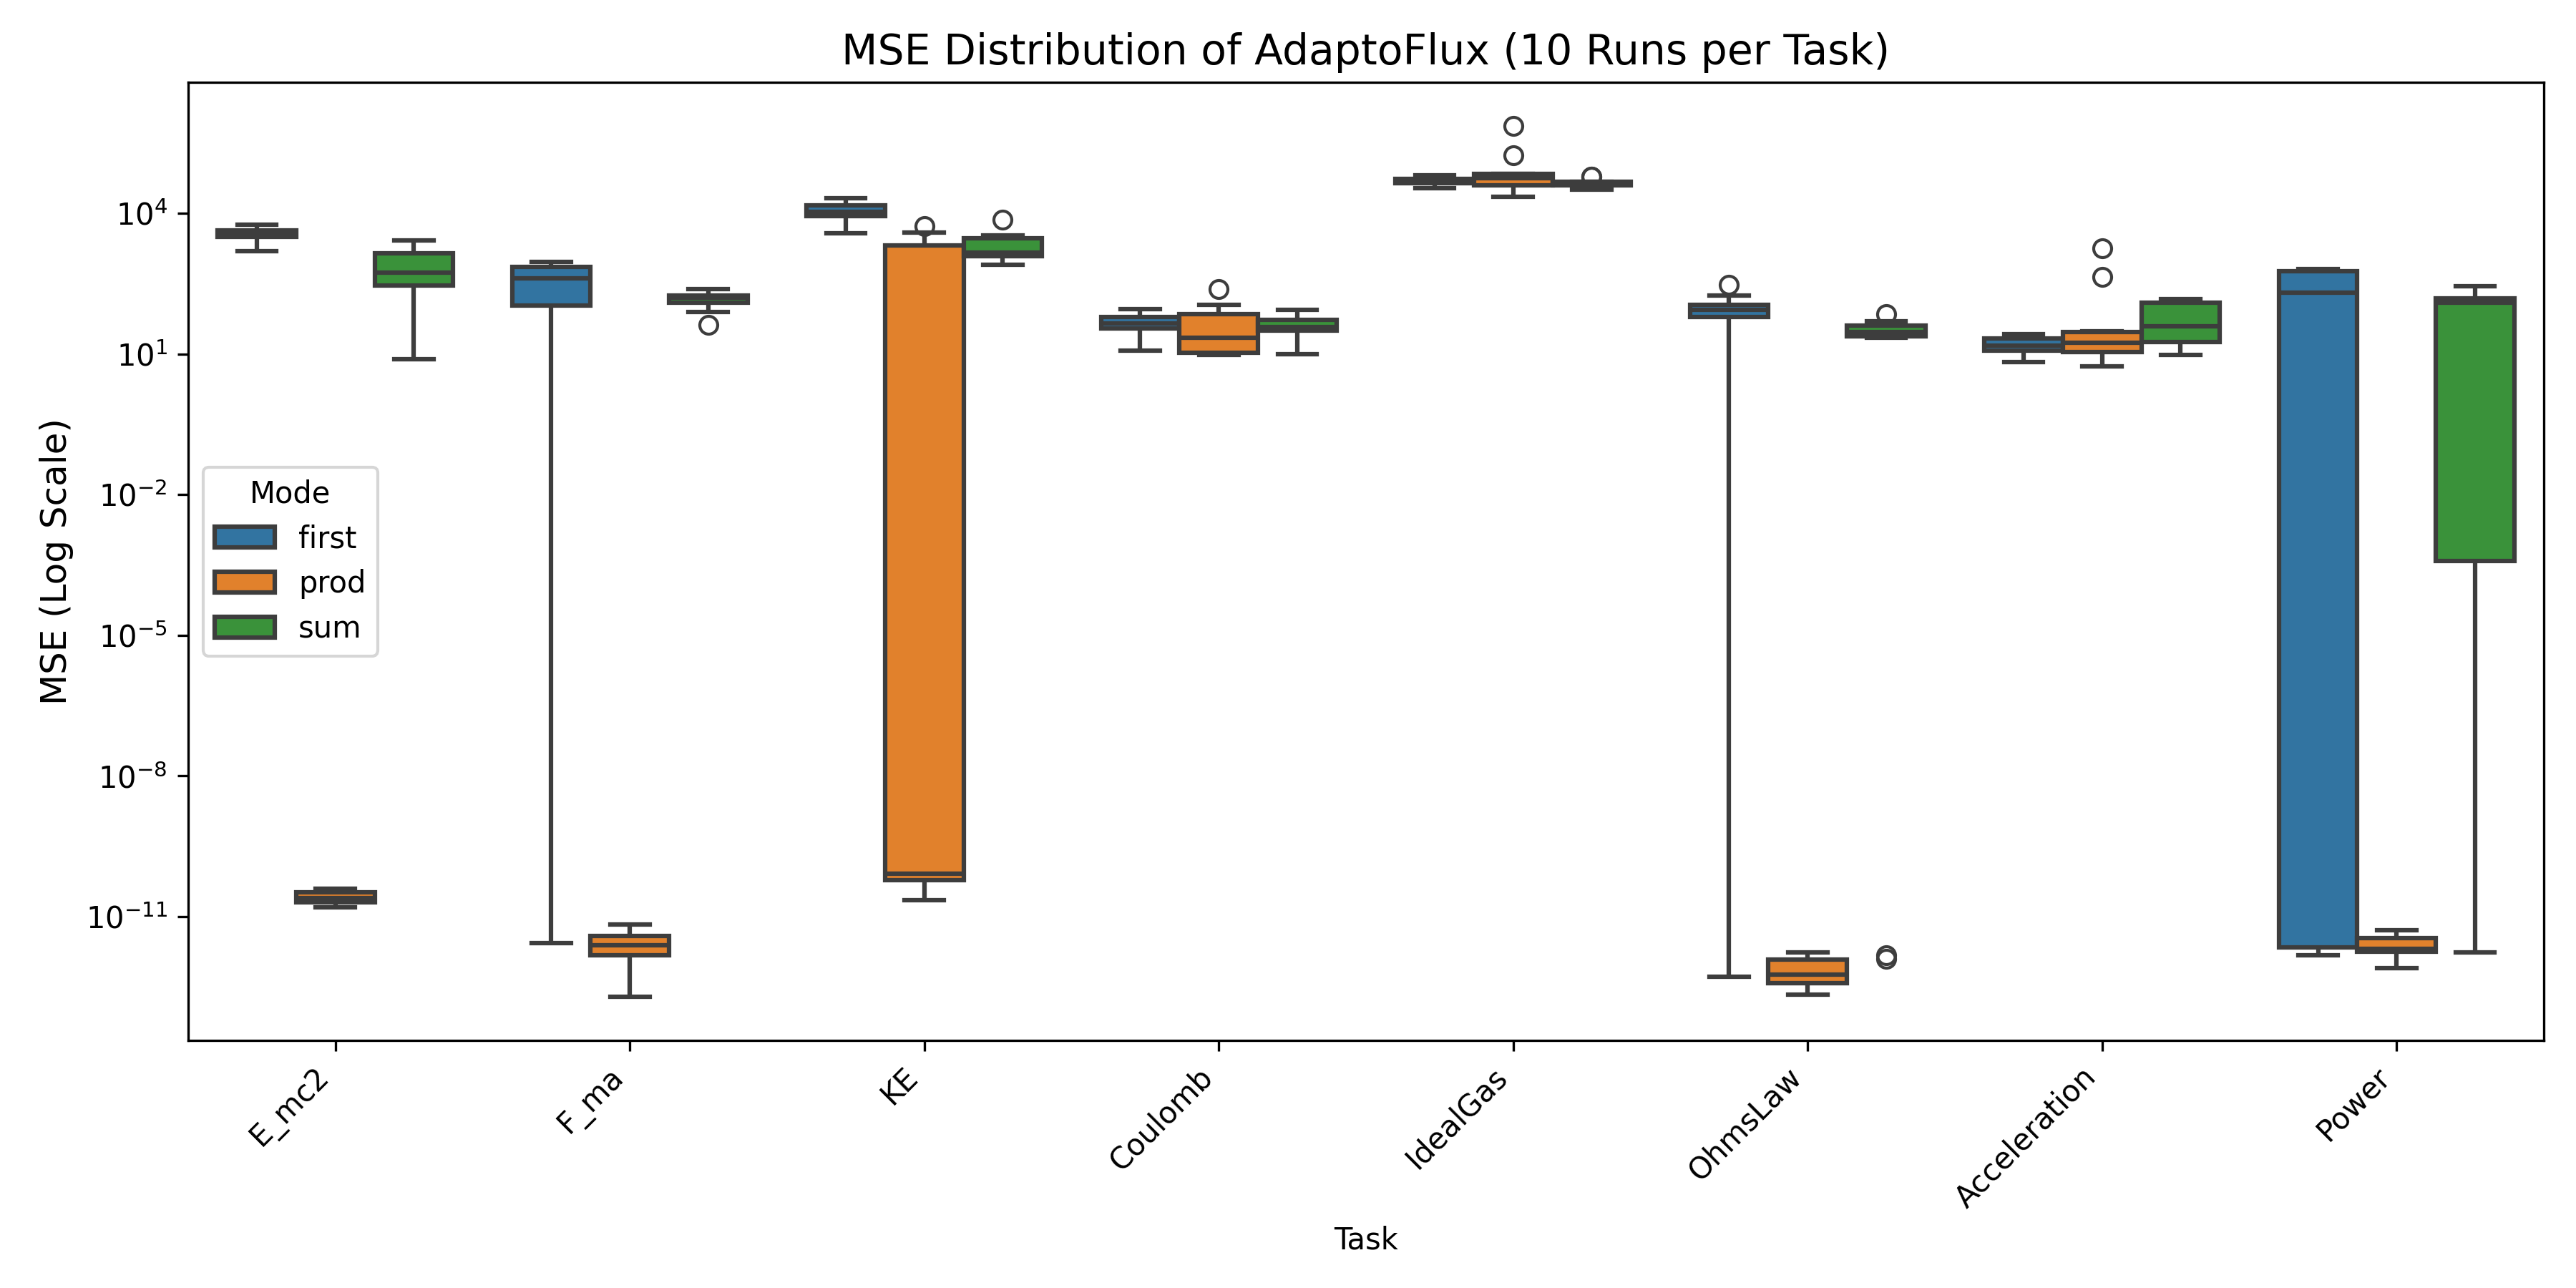
\includegraphics[width=\linewidth]{images/ExternalBaselines/atf_mse_distribution_boxplot.png} 
    \caption{Distribution of Mean Squared Error (MSE) for AdaptoFlux across 8 Feynman tasks over 10 independent runs. The log-scale y-axis emphasizes the stability of the \texttt{prod} mode in multiplication tasks versus the high variance in complex tasks.}
    \label{fig:mse_distribution}
\end{figure}

\begin{figure}[htbp]
    \centering
    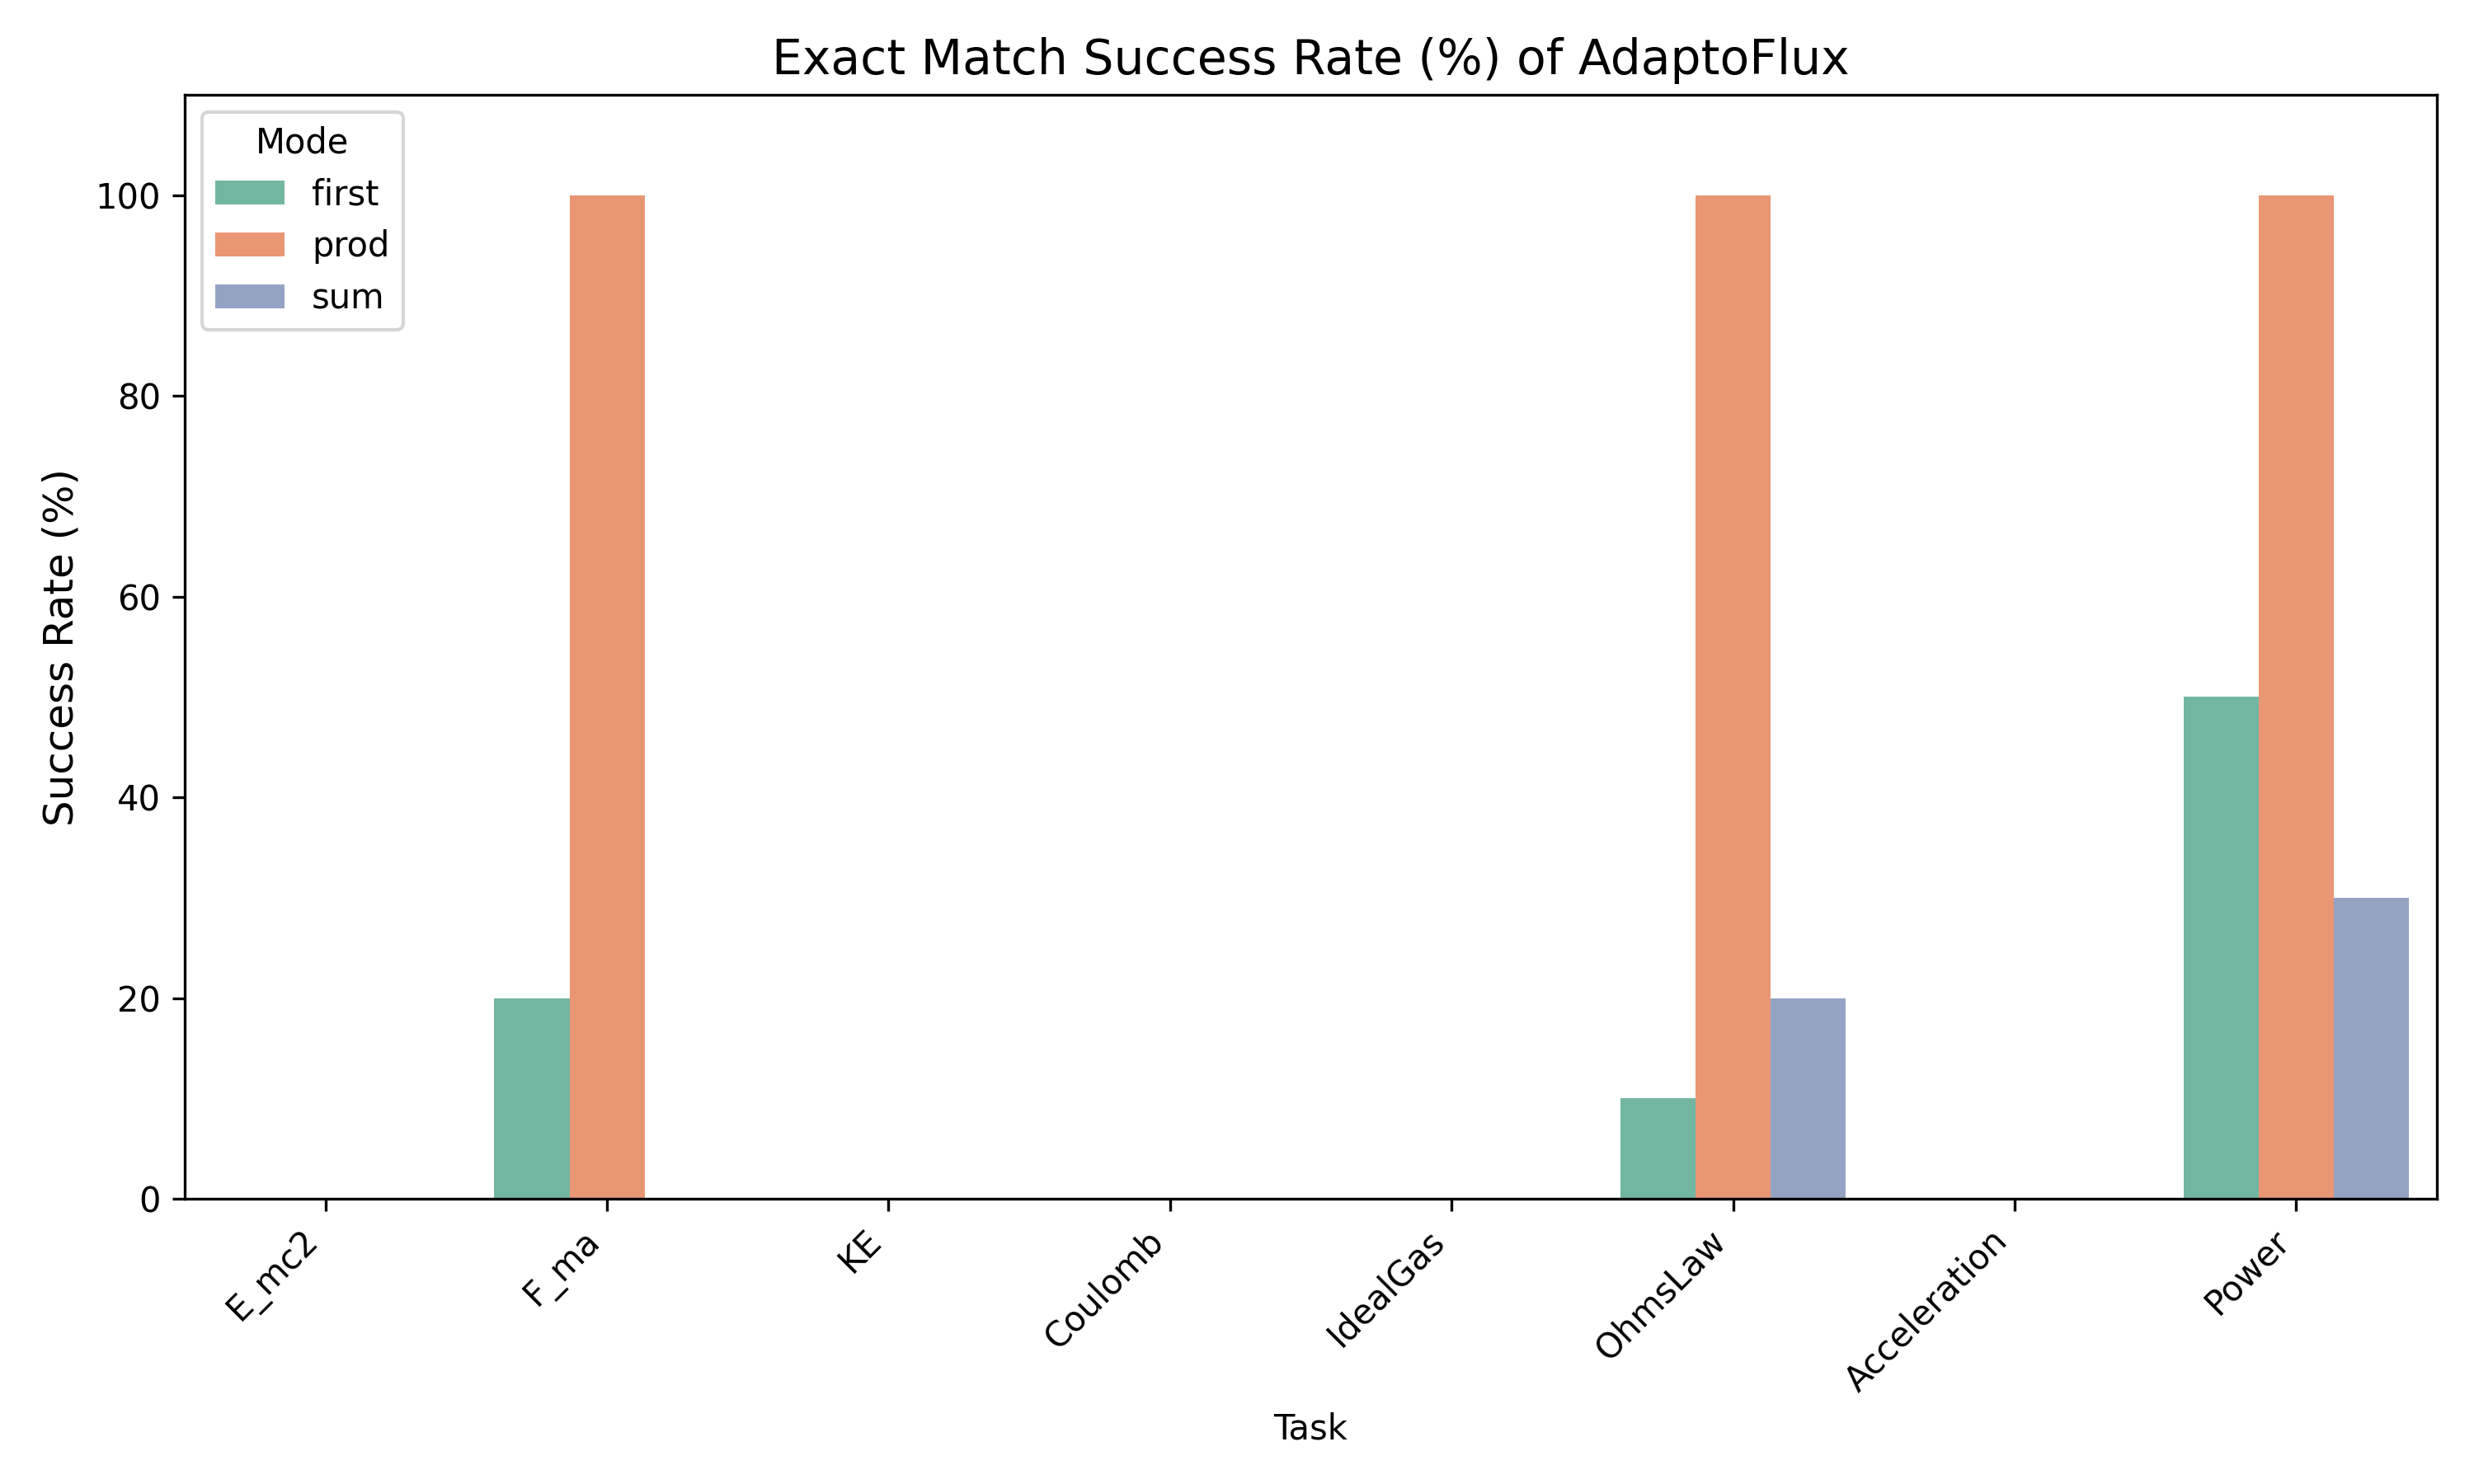
\includegraphics[width=\linewidth]{images/ExternalBaselines/atf_success_rate_bars.png}
    \caption{Exact Symbolic Match Success Rate (\%) for AdaptoFlux across different collapse modes. The \texttt{prod} mode demonstrates robust stability (100\% success) on multiplication-dominated tasks, whereas other modes show significant inconsistency.}
    \label{fig:success_rate}
\end{figure}

\begin{table}[htbp]
    \centering
    \small % 或者 \footnotesize，根据空间情况选择
    \setlength{\tabcolsep}{3pt} % 默认是 6pt，减小列间距
    \caption{AdaptoFlux performance with collapse=\texttt{first} over 10 independent runs. Values report Mean $\pm$ Std for MSE and Runtime, along with Median, Min MSE, and Exact Match Success Rate.}
    \label{tab:atf_stats_first}
    \begin{tabular}{lcccccc}
        \toprule
        Task & MSE (Mean $\pm$ Std) & Median & Min & Success Rate (\%) & Runtime (s) $\pm$ Std \\
        \midrule
        E\_mc2       & $3.50e+03 \pm 1.21e+03$ & $3.47e+03$ & $1.55e+03$ & 0.0  & $3.10 \pm 1.75$ \\
        F\_ma        & $4.31e+02 \pm 3.28e+02$ & $4.13e+02$ & $2.77e-12$ & 20.0 & $3.39 \pm 6.96$ \\
        KE           & $1.16e+04 \pm 5.28e+03$ & $1.09e+04$ & $3.71e+03$ & 0.0  & $10.14 \pm 11.53$ \\
        Coulomb      & $4.78e+01 \pm 2.11e+01$ & $4.49e+01$ & $1.19e+01$ & 0.0  & $7.90 \pm 8.58$ \\
        IdealGas     & $4.87e+04 \pm 8.04e+03$ & $4.70e+04$ & $3.47e+04$ & 0.0  & $7.44 \pm 4.85$ \\
        OhmsLaw      & $1.04e+02 \pm 7.77e+01$ & $8.71e+01$ & $5.28e-13$ & 10.0 & $1.51 \pm 1.72$ \\
        Acceleration & $1.58e+01 \pm 6.16e+00$ & $1.49e+01$ & $6.68e+00$ & 0.0  & $2.41 \pm 3.23$ \\
        Power        & $2.81e+02 \pm 2.88e+02$ & $2.05e+02$ & $1.49e-12$ & 50.0 & $0.54 \pm 0.30$ \\
        \bottomrule
    \end{tabular}
\end{table}

\begin{table}[htbp]
    \centering
    \small % 或者 \footnotesize，根据空间情况选择
    \setlength{\tabcolsep}{3pt} % 默认是 6pt，减小列间距
    \caption{AdaptoFlux performance with collapse=\texttt{prod} over 10 independent runs. This mode demonstrates the highest stability and success rate in multiplication-dominated tasks (F\_ma, OhmsLaw, Power).}
    \label{tab:atf_stats_prod}
    \begin{tabular}{lcccccc}
        \toprule
        Task & MSE (Mean $\pm$ Std) & Median & Min & Success Rate (\%) & Runtime (s) $\pm$ Std \\
        \midrule
        E\_mc2       & $2.64e-11 \pm 7.80e-12$ & $2.53e-11$ & $1.59e-11$ & 0.0  & $0.07 \pm 0.01$ \\
        F\_ma        & $2.88e-12 \pm 1.96e-12$ & $2.42e-12$ & $1.93e-13$ & 100.0 & $0.02 \pm 0.00$ \\
        KE           & $1.31e+03 \pm 1.86e+03$ & $8.29e-11$ & $2.27e-11$ & 0.0  & $2.61 \pm 3.14$ \\
        Coulomb      & $5.65e+01 \pm 6.85e+01$ & $2.25e+01$ & $9.40e+00$ & 0.0  & $9.20 \pm 3.30$ \\
        IdealGas     & $1.28e+05 \pm 2.04e+05$ & $5.55e+04$ & $2.25e+04$ & 0.0  & $15.17 \pm 7.40$ \\
        OhmsLaw      & $8.04e-13 \pm 5.15e-13$ & $5.89e-13$ & $2.21e-13$ & 100.0 & $0.02 \pm 0.00$ \\
        Acceleration & $2.36e+02 \pm 5.36e+02$ & $1.73e+01$ & $5.38e+00$ & 0.0  & $11.62 \pm 4.05$ \\
        Power        & $2.65e-12 \pm 1.41e-12$ & $2.07e-12$ & $8.05e-13$ & 100.0 & $0.02 \pm 0.00$ \\
        \bottomrule
    \end{tabular}
\end{table}

\begin{table}[htbp]
    \centering
    \small % 或者 \footnotesize，根据空间情况选择
    \setlength{\tabcolsep}{3pt} % 默认是 6pt，减小列间距
    \caption{AdaptoFlux performance with collapse=\texttt{sum} over 10 independent runs. Generally exhibits higher variance and lower success rates compared to \texttt{prod}, particularly in complex tasks.}
    \label{tab:atf_stats_sum}
    \begin{tabular}{lcccccc}
        \toprule
        Task & MSE (Mean $\pm$ Std) & Median & Min & Success Rate (\%) & Runtime (s) $\pm$ Std \\
        \midrule
        E\_mc2       & $8.84e+02 \pm 7.94e+02$ & $5.33e+02$ & $7.73e+00$ & 0.0  & $154.79 \pm 201.62$ \\
        F\_ma        & $1.50e+02 \pm 5.70e+01$ & $1.57e+02$ & $4.11e+01$ & 0.0  & $12.78 \pm 20.35$ \\
        KE           & $2.33e+03 \pm 1.88e+03$ & $1.44e+03$ & $7.84e+02$ & 0.0  & $159.76 \pm 153.73$ \\
        Coulomb      & $4.27e+01 \pm 2.15e+01$ & $3.81e+01$ & $9.73e+00$ & 0.0  & $7.52 \pm 5.12$ \\
        IdealGas     & $4.38e+04 \pm 9.34e+03$ & $4.21e+04$ & $3.14e+04$ & 0.0  & $11.50 \pm 19.96$ \\
        OhmsLaw      & $3.06e+01 \pm 1.99e+01$ & $2.98e+01$ & $1.26e-12$ & 20.0 & $4.82 \pm 3.52$ \\
        Acceleration & $6.52e+01 \pm 5.45e+01$ & $3.84e+01$ & $9.58e+00$ & 0.0  & $19.94 \pm 40.29$ \\
        Power        & $1.01e+02 \pm 9.30e+01$ & $1.22e+02$ & $1.76e-12$ & 30.0 & $25.39 \pm 42.22$ \\
        \bottomrule
    \end{tabular}
\end{table}

\subsection{Analysis of Core Findings}

\begin{enumerate}
    \item \textbf{Under the restricted setting, the substrate recovered exact symbolic structures in multiplication-dominated tasks}: for F\_ma, OhmsLaw, Power, E\_mc2, and KE, the \texttt{prod} mode not only reached high numerical precision (MSE $\sim 10^{-13}$--$10^{-11}$) but also produced computation graphs that were \textbf{algebraically equivalent} to the target formulas under symbolic verification (Table~\ref{tab:symbolic_exact_match}), matching the specialized reference systems on these tasks. This demonstrates that the GDFG representation retains basic symbolic expressiveness---it can synthesize correct program structure, including formulas with explicit constants---even when stripped of method imports and driven by a lightweight probe.
    
    \item \textbf{ATF can correctly combine input variables containing constants, but its performance is highly sensitive to search configuration}: In the Kinetic Energy (KE) task, where the constant $0.5$ in the target formula $0.5 \cdot m \cdot v^2$ is provided as an independent input dimension, AdaptoFlux successfully constructed the correct multiplication chain ($x_2 \cdot x_0 \cdot x_1 \cdot x_1$) in \texttt{prod} mode, achieving algebraic equivalence (Table~\ref{tab:symbolic_exact_match}); whereas it failed completely in \texttt{sum} or \texttt{first} modes (Tables~\ref{tab:baselines_sum}, \ref{tab:baselines_first}). This contrast clearly indicates that \textbf{AdaptoFlux's search effectiveness strongly depends on configurations aligned with the mathematical structure of the task}. For three-variable nonlinear tasks like IdealGas and Coulomb, ATF has not yet recovered the correct symbolic structure under the current uniform \texttt{prod} mode setting; however, manual inspection of its best solutions reveals that the output programs often miss only one or two key operations (such as a division or variable copy). This suggests that success rates could be significantly improved by introducing more flexible collapse strategies, increasing graph depth, or expanding method pool capacity---but to maintain fair comparison with baselines, this experiment did not adjust hyperparameters or search strategies for specific tasks.
    
    \item \textbf{The choice of Collapse mode is critical}: The \texttt{prod} mode performed excellently in multiplication-like tasks, while \texttt{first} and \texttt{sum} modes were generally poor. This reveals a key design principle of AdaptoFlux: the output aggregation strategy must align with the mathematical structure of the target task.
    
    \item \textbf{Inspectable errors}: the recovered program graphs (Fig.~\ref{fig:atf_graphs}) expose which variables and operations contribute to each prediction, including cases with substantial numerical error.
\end{enumerate}

\subsection{Conclusion}

With \texttt{prod} aggregation, the original AdaptoFlux probes recovered algebraically equivalent expressions for F\_ma, OhmsLaw, Power, E\_mc2 and KE. Recovery depended strongly on the aggregation mode and on the supplied operators. PySR and gplearn also solved Coulomb, IdealGas and Acceleration, where the tested ATF configurations failed. Together, the numerical and symbolic checks identify both successful compositions and the remaining search gaps under this arithmetic pool.

\section{Hand-Crafted Snake Controller}
\label{app:snake_controller}

To verify AdaptoFlux's native support for side-effectful actions, we manually constructed a Generalized Data Flow Graph (GDFG) to control an agent in the classic Snake game. This entire process required no training or parameter tuning.

As shown in Figure~\ref{fig:snake_gdfg}, the graph consists of four logical layers:
\begin{itemize}
    \item \textbf{Input Extraction Layer}: Reads the current game state (e.g., snake head position, food coordinates, presence of hazards ahead);
    \item \textbf{Perception and Reasoning Layer}: Computes spatial relationships (e.g., ``hazard ahead,'' ``food to the right'');
    \item \textbf{Decision Logic Layer}: Executes symbolic rules based on pure functions from the method pool (e.g., ``if hazard ahead, then turn left'');
    \item \textbf{Action Execution Layer}: Invokes methods with side effects (such as \texttt{turn\_left()}, \texttt{move\_forward()}), directly modifying the environment state via \texttt{SNAKE\_STATE.set\_action()}.
\end{itemize}

The action layer contains three alternatives, \texttt{turn\_left}, \texttt{turn\_right} and \texttt{go\_straight}, whose Boolean permissions are mutually exclusive. They are not connected as a sequential action chain: only the permitted branch updates the environment in a tick. This application-level exclusion explains the behavior of the original controller. The revised executor additionally supports declared resource ordering for graphs with several conflicting active operations. The stored graph remains static, and one graph evaluation selects each step's action.

Although this controller is simple in structure and unoptimized, it operates stably for hundreds of steps in a $10\times10$ grid, effectively avoiding self-collision and continuously tracking food. This result validates the core claim of AdaptoFlux: \textbf{it provides a unified and executable underlying framework for both pure computation and interactive behavior}---as illustrated by the explicit state-changing action interface. We have provided the running video of this model in the supplementary materials.

\begin{figure}[htbp]
    \centering
    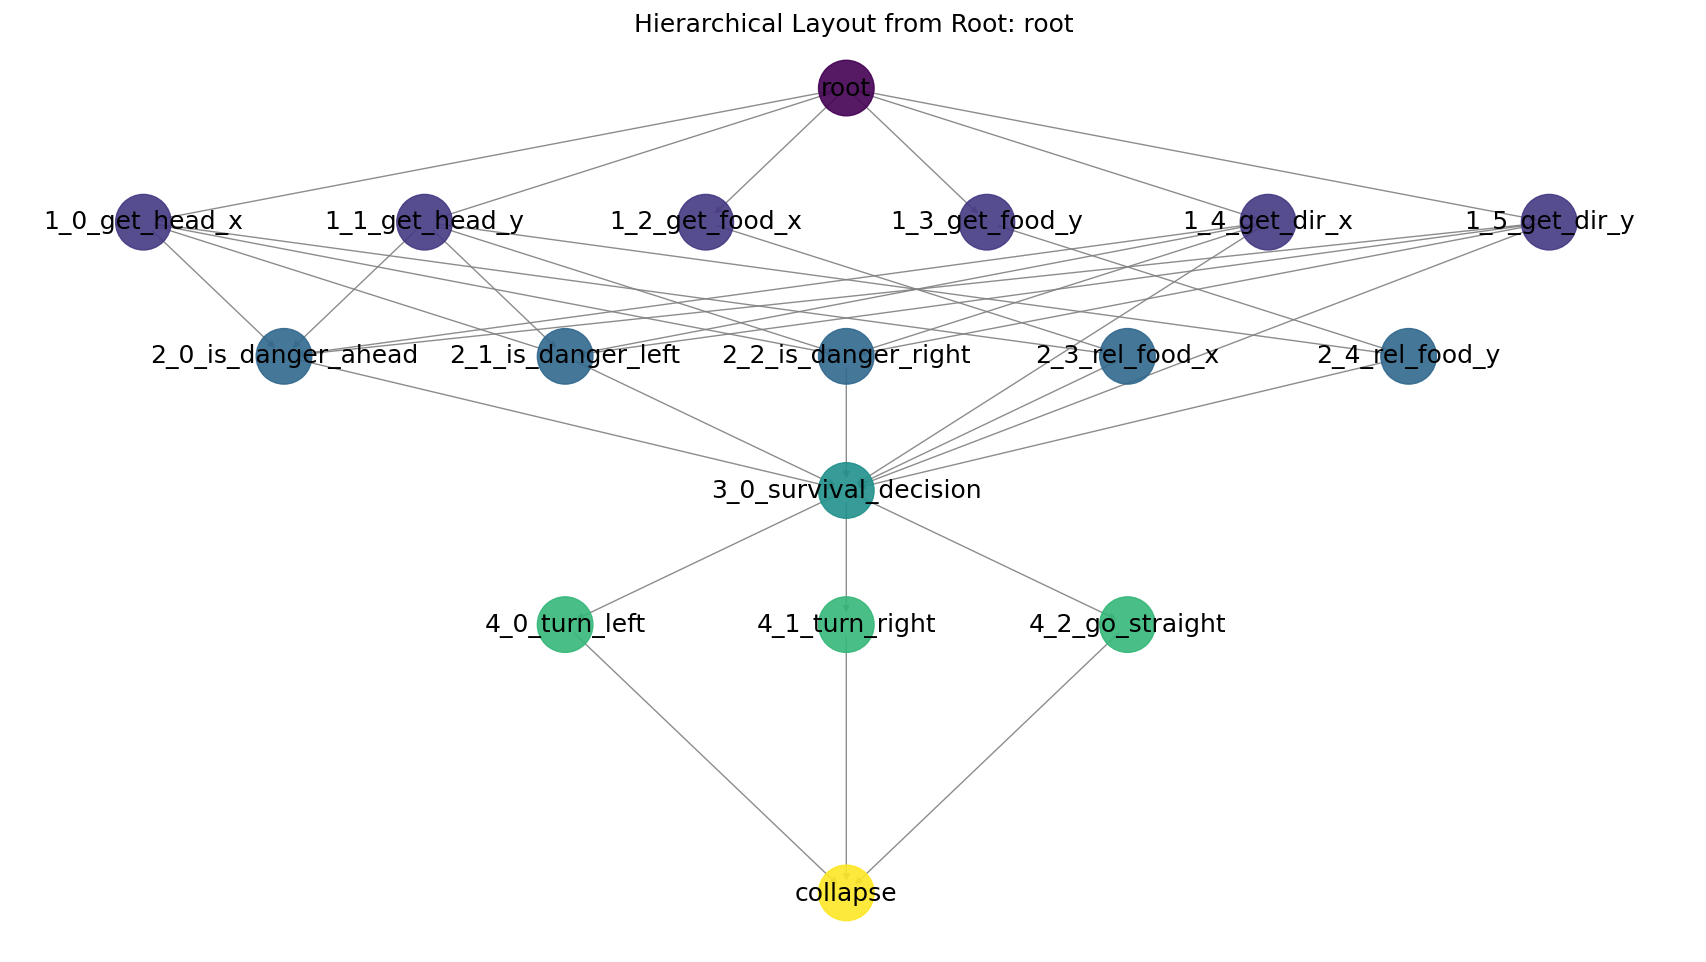
\includegraphics[width=0.8\textwidth]{images/snake/snake.png}
    \caption{Hand-crafted GDFG for the Snake agent. Action-layer nodes execute operations with side effects (such as \texttt{turn\_left}), directly modifying the environment state. Mutually exclusive permissions select one action branch within the same graph as the pure computations.}
    \label{fig:snake_gdfg}
\end{figure}

% ==============================================================================
% APPENDIX F: Implementation Details and Reproducibility Guide
% (Automatically numbered as F by LaTeX if previous was E)
% ==============================================================================

\section{Implementation Details and Reproducibility Guide}
\label{app:impl-details}

\noindent Appendix~\ref{sec:appendix_experiments} records the original five experiment categories. The directory map below identifies their configurations, method pools, logs and execution scripts. The supplementary revision experiments and their frozen protocols are described in Appendices~\ref{app:revision_types}--\ref{app:revision_capacity}.

\subsection{Method Pool Interface and Decorator Implementation}
The formal definition $m = \langle \text{impl}, \sigma_{\text{in}}, \sigma_{\text{out}}, \mathcal{M} \rangle$ from Main Text §~\ref{subsec:method_pool} is bound in the prototype system via the \texttt{@method\_profile} decorator. This mechanism transforms host language functions into atomic units parseable by the framework, automatically injecting type routing and metadata:

\begin{lstlisting}[language=Python, caption={Original decorator interface used by the historical experiments}]
def method_profile(
    output_count: int | None = None,
    input_types=None,
    output_types=None,
    group: str = "default",
    weight: float = 1.0,
    is_internal_decorator: bool = False,
    vectorized: bool = False
):
    def decorator(func):
        func.output_count = output_count if output_count else len(output_types or [])
        func.input_types = input_types or []
        func.output_types = output_types or []
        func.group = group
        func.weight = weight
        func.is_internal_decorator = is_internal_decorator
        func.vectorized = vectorized
        return func
    return decorator
method_profile.is_internal_decorator = True
\end{lstlisting}

\noindent\textbf{Mapping Relationship:} Attributes injected by the decorator directly correspond to the formal tuple $\mathcal{M}$. When constructing graph edges, the framework enforces hard type-constrained routing by comparing \texttt{output\_types} with downstream nodes' \texttt{input\_types}; \texttt{group} and \texttt{weight} drive dynamic view projection and probe sampling, and neither participates in the definition of $\Omega$ (Appendix~\ref{app:metadata_role}).

\noindent The revised decorator adds \texttt{pure}, \texttt{reads} and \texttt{writes} declarations. These are execution contracts used to derive control dependencies; \texttt{group} and \texttt{weight} remain search preferences. Appendix~\ref{app:revision_effects} describes how the declarations and execution-mode setting are preserved.

\subsection{Experiment Configuration and Repository Path Mapping}
To ensure reproducibility transparency, all experiments adopt a self-contained directory structure. Table~\ref{tab:repo-mapping} establishes a precise index between main text experiments and repository assets.

\noindent\textbf{Path Note:} All scripts are located in the \path{experiments/} directory of the anonymous repository. The table below lists relative paths and core output files.

\begin{table}[H]
\raggedright
\caption{Experiment Configuration and Repository Path Mapping}
\label{tab:repo-mapping}

% 使用标准的 description 环境
% leftmargin=* 让列表左对齐，避免缩进过多
\begin{description}[leftmargin=*, style=nextline, itemsep=5pt, parsep=2pt]
    
    % 关键：手动加粗标签，确保它可见
    \item[\textbf{LayerGrow (Sec.~\ref{subsec:layergrow_validation}, Appx.~\ref{sec:appendix_exp1})}]
        \small % 内容用小字
        \path{LayerGrowTrainer_exp1/main.py} \\
        $\rightarrow$ \texttt{experiment\_results\_summary.csv}

    \item[\textbf{Knowledge Transfer (Sec.~\ref{subsec:graphevo_validation}, Appx.~\ref{sec:appendix_exp2})}]
        \small
        \path{GraphEvo_exp3/exp3_main.py} \\
        $\rightarrow$ \path{exp3_results/summary_table.csv}

    \item[\textbf{Minimal Stateful Attractor (Sec.~\ref{subsec:stateful_synthesis}, Appx.~\ref{sec:appendix_exp4})}]
        \small
        \path{minimal_stateful_comparison/run_comparison.py} \\
        $\rightarrow$ \path{logs/} + \path{results/stateful_synthesis_comparison.png}

    \item[\textbf{Topology-Aware Parallel (Appx.~\ref{sec:appendix_exp3})}]
        \small
        \path{PipelineParallel_exp2/scripts/benchmark.py} \\
        $\rightarrow$ \path{PipelineParallel_exp2/results/}

    \item[\textbf{Geometric Classification (Appx.~\ref{sec:appendix_geo_ablation})}]
        \small
        \leavevmode\par
        \begin{itemize}[topsep=0pt,partopsep=0pt,itemsep=0pt,parsep=0pt]
            \item \path{Combined_exp4_circles/test_combined_trainer.py}
            \item \path{Combined_exp4_spiral/test_combined_trainer.py}
            \item \path{Combined_exp4_spiral_no_Trigonometric/}\\
                  \path{test_combined_trainer.py}
        \end{itemize}
        $\rightarrow$ \path{experiment_results/} (regenerated by the script; $\approx$0.5\,GB per task, not shipped)

    \item[\textbf{Feynman Regression (Appx.~\ref{sec:appendix_baseline_comparison})}]
        \small
        \path{ExternalBaselines/run_baselines_*.py} \\
        $\rightarrow$ \path{ExternalBaselines/results/}

    \item[\textbf{Snake Controller (Appx.~\ref{app:snake_controller})}]
        \small
        \path{embodied_snake/snake_main.py} + \texttt{snake.json}\textsuperscript{\dag} \\
        $\rightarrow$ \texttt{snake\_demo.mp4}

\end{description}

\vspace{1em}
\noindent\textsuperscript{\dag}\footnotesize{Note: \texttt{snake.json} is a hand-crafted GDFG configuration file (not learned).}

\end{table}



\noindent\textbf{Note:} All paths in the table are relative to the anonymous code repository root. Output artifact types vary by task, including: run logs and trajectories (\texttt{.log}/\texttt{.json}), statistical metric tables (\texttt{.csv}), execution demo videos (\texttt{.mp4}), and graph configuration files. The complete directory structure, environment dependencies, and one-click reproduction guides are detailed in the \texttt{README.md} file in the repository or supplementary materials.

Raw result tables---the LayerGrow configuration summary, the knowledge-transfer summary, the parallel-scheduling benchmark, the Feynman-baseline results and the minimal-stateful run logs---are shipped, so that the reported statistics can be recomputed independently. Larger outputs are regenerated by the corresponding scripts: the \path{training_log.json} files under \path{exp_max_layers_*/run_*/}, the contents of \path{exp3_results/<config>/rep<k>/}, \path{models/} and \path{plots/}, and the three geometric-classification \path{experiment_results/} directories ($\approx$0.5\,GB each). These outputs are excluded from the supplement for size.

\subsection{Reproduction Environment and Running Guide}
\noindent\textbf{Software Dependencies:} AdaptoFlux is developed based on Python 3.12+. The complete dependency list is in \texttt{requirements.txt} at the repository root, installable via \texttt{pip install -r requirements.txt}. The framework executes entirely on CPU, with no GPU dependencies.
\noindent\textbf{Compute Resources:} All experiments were executed on standard workstations with multi-core CPUs and 60GB RAM. No GPU was used. Specifically, the parallel scalability experiments utilized a server with 32 CPU cores to evaluate multi-threading performance. The total wall-clock time to reproduce all main experimental results sequentially is estimated to be less than one week.
\noindent\textbf{Statistical Protocol Alignment:} The random seed allocation, repetition counts, and success determination thresholds for each experiment strictly follow the regulations outlined in the Main Text and Appendices. All raw logs have been fully exported, supporting independent recalculation of means, variances, and success rates.

% ==============================================================================
% APPENDIX G: Semantic Taxonomy of the Method Pool
% ==============================================================================

\section{Semantic Taxonomy of the Method Pool}
\label{app:method-pool-semantics}

Main Text Section~\ref{subsec:method_pool} introduced the engineering implementation of the Method Pool $\mathcal{Q}$ and its metadata-driven architecture. This section further provides two typical classification examples from a semantic perspective to demonstrate the flexibility and expressive potential of the method pool in handling heterogeneous operations. It is emphasized that the following classification systems serve only as \textbf{Illustrative Examples}, aiming to elucidate how the framework establishes structural order through metadata, rather than imposing hard constraints on the method pool. AdaptoFlux natively supports users defining arbitrary orthogonal classification views based on task requirements (e.g., by hardware affinity, computational complexity, or semantic role).

\subsection{Example 1: Heterogeneous Operation Classification Based on Functional Attributes}

To natively bridge pure computation and state interaction, AdaptoFlux's method pool $\mathcal{Q}$ supports semantically tagging methods from two orthogonal functional dimensions: \textbf{Mapping} and \textbf{Action}. It is emphasized that these two dimensions are not mutually exclusive sets but allow overlapping feature labels---a method can simultaneously possess deterministic input-output mapping relationships and side effects that change system state or environment. This flexibility allows the framework to uniformly model a wide range of operations from pure mathematical formulas to embodied control instructions.

\begin{description}
    \item[Mapping Perspective ($\mathcal{Q}_F$)] Focuses on the input-output transformation relationship $f: \text{Input} \to \text{Output}$. For a pure deterministic implementation, these methods compute repeatable outputs and support symbolic regression and feature extraction; declared types constrain their connections. Even if a method contains side effects, its mapping part can still be independently analyzed for data flow reasoning.
    \item[Action Perspective ($\mathcal{Q}_O$)] Focuses on the effect produced on the system state $\mathbf{s}_{t+1} = \Phi(\mathbf{s}_t, \mathbf{x}_t)$ or the external environment after method execution. Such methods introduce time dependency and state evolution capabilities, forming the core of building dynamic systems and embodied agents.
\end{description}

\paragraph{Example Comparison and Overlap Cases}
\begin{itemize}
    \item \textbf{Pure Mapping Example}: $f(x) = x \times \frac{9}{5} + 32$ (Celsius to Fahrenheit). No state dependency, no side effects, only returns calculation results.
    \item \textbf{Pure Action Example}: \texttt{send\_notification(msg)}. The primary purpose is to execute I/O operations; the return value is usually secondary or empty, with the core being the triggered external effect.
    \item \textbf{Mixed Case Example}: \texttt{update\_and\_return\_score(state, action)}. This method both calculates a numerical score based on current state and action (mapping characteristic) and records the action in the historical trajectory while updating the environment state (action characteristic). AdaptoFlux allows such methods to simultaneously assume the dual roles of data transmission and state evolution in the graph.
\end{itemize}

\subsubsection{Subdivision of Action Pool by Side-Effect Scope}

The action pool $\mathcal{Q}_O$ can be further subdivided based on the object affected by side effects (see Table~\ref{tab:supp_action_scope}). This classification determines the state update strategy of the graph execution engine during time-step unrolling.

\begin{table}[htbp]
\small % 或者 \footnotesize，根据空间情况选择
\setlength{\tabcolsep}{3pt} % 默认是 6pt，减小列间距
\centering
\caption{[Example] Action Pool Classification by Side-Effect Scope}
\label{tab:supp_action_scope}
\renewcommand{\arraystretch}{1.3}
\begin{tabular}{|l|c|c|p{5cm}|}
\hline
\textbf{Type} & \textbf{Affects Self-State} & \textbf{Affects External Env} & \textbf{Typical Application} \\ \hline
Self Side-Effect & \checkmark & $\times$ & Internal counter updates, memory storage \\ \hline
Env Side-Effect & $\times$ & \checkmark & API calls, robot movement commands \\ \hline
Dual Side-Effect & \checkmark & \checkmark & Perception-action loops in embodied intelligence \\ \hline
\end{tabular}
\end{table}

\subsection{Example 2: Reversibility Classification Based on Information Flow Attributes}

For the function pool $\mathcal{Q}_F$, we can classify methods based on the ability to restore inputs from outputs. This perspective demonstrates the theoretical potential of the method pool in supporting reverse reasoning or lossless encoding tasks.

\begin{table}[htbp]
\small
\centering
\caption{Function Pool Classification by Reversibility}
\label{tab:supp_func_reversibility}
\renewcommand{\arraystretch}{1.3}

% 使用 tabularx，去掉竖线，使用 @{} 去除左右多余空白
\begin{tabularx}{\linewidth}{@{} l X X @{}} 
\toprule
\textbf{Type} & \textbf{Characteristic} & \textbf{Reverse Deduction Ability} \\ 
\midrule
Non-Reversible (N) & Many-to-One Mapping & Cannot uniquely restore; only probabilistic inference \\ 
Conditionally Reversible (CR) & Requires partial input or context & Can uniquely restore remaining inputs given partial inputs \\ 
Fully Reversible (FR) & One-to-One Mapping (Bijective) & Can uniquely restore original inputs solely from output \\ 
\bottomrule
\end{tabularx}
\end{table}

\paragraph{Fully Reversible Function Pool Example}
Based on the Fundamental Theorem of Arithmetic, construct the function $f(a, b) = 2^a \cdot 3^b$ ($a,b \in \mathbb{N}$). Due to the uniqueness of prime factorization, any output $y$ can be uniquely inverted to $(a, b)$. Such functions have theoretical value in scenarios requiring lossless state recovery or encoding/decoding, demonstrating AdaptoFlux's ability to handle complex mathematical properties.

\subsection{Dynamic Construction and Task-Adaptive Filtering}

The above classifications are not static labels but the foundation for dynamic filtering. AdaptoFlux allows dynamically constructing sub-pools through metadata projection. This is a search-side restriction that leaves $\Omega$ unchanged (Appendix~\ref{app:metadata_role}).

\subsubsection{Method Registration and Global State}
Methods are registered via the \texttt{@method\_profile} decorator and can be associated with global state storage (such as memory dictionaries). This allows action functions to share information across time steps, achieving long-term memory without hard-coding state variables.

\subsubsection{Task-Adaptive Sub-Pool Filtering Mechanism}
Facing large-scale base method pools, the search space grows exponentially. To improve efficiency, subset filtering mechanisms can be introduced. Here we provide a simple example using a Genetic Algorithm (GA) to optimize method subsets:
\begin{enumerate}
    \item \textbf{Initialization}: Randomly sample multiple fixed-size method subsets.
    \item \textbf{Evaluation}: Run lightweight \texttt{LayerGrow} on each subset, using validation set accuracy as fitness.
    \item \textbf{Evolution}: Iteratively optimize through selection, crossover, and mutation, eliminating redundant or interfering operators.
\end{enumerate}
This process aims to find a "semantically complete and minimal" sub-pool. The performance fluctuation of \texttt{CombinedTrainer\_periodic} in Appendix~\ref{sec:appendix_geo_ablation} reflects this trade-off: excessive compression may lead to the loss of key semantic primitives (such as trigonometric functions), thereby causing semantic collapse of the expression space. This further confirms that the composition of the method pool has a decisive impact on navigation efficiency.

\subsection{Hypothesis Class and the Formal Role of Metadata}
\label{app:metadata_role}

\paragraph{Data compatibility and execution contracts.}
For a registered pool $\mathrm{Q}$ and type system $\Sigma$, Eq.~\ref{eq:expression_space} defines the admissible data DAGs. Port signatures constrain which outputs may supply which arguments, and acyclicity admits a topological schedule. These checks concern declared interfaces. State-dependent execution additionally uses the program contract $P=(G,\pi,E_c)$: a frozen semantic order $\pi$ and control dependencies $E_c$ derived from declared resource accesses.

\paragraph{Search preferences select a view.}
For a filter $\phi$, define $\mathrm{Q}_{\mathrm{view}}(\phi)=\{m\in\mathrm{Q}\mid\phi(\mathrm{M}_m)=\mathrm{True}\}$. Filtering by search tags such as \texttt{group} restricts the examined data graphs to $\Omega_{\mathrm{Q}_{\mathrm{view}},\Sigma}\subseteq\Omega_{\mathrm{Q},\Sigma}$. Sampling weights alter the distribution of proposals within that view. These preferences are distinct from \texttt{pure}/\texttt{reads}/\texttt{writes}: changing an effect declaration changes the execution contract and may change the required schedule.

\begin{table}[htbp]
\centering\small
\caption{Interface constraints, execution contracts and search preferences have different roles.}
\label{tab:hard-soft}
\begin{tabularx}{\linewidth}{@{}p{0.23\linewidth}p{0.22\linewidth}X@{}}
\toprule
Mechanism & Role & Operational effect \\
\midrule
Type signatures and ports & Data compatibility & Admit connections to declared argument positions; the three-condition experiment varies these signatures. \\
Acyclicity & Data schedulability & Reject cycles in the stored data graph. \\
Read/write declarations; saved order & State execution contract & Determine control dependencies when effect ordering is enabled; preserve the selected order through evaluation and persistence. \\
Group and search tags & Candidate view & Select the subset of registered methods exposed to a probe. \\
Sampling weights & Proposal preference & Alter how often methods are proposed. \\
Reuse history & Search bookkeeping & Guide extraction and reuse; extracted methods retain their execution contracts. \\
\bottomrule
\end{tabularx}
\end{table}

\paragraph{Evidence.}
The type-prior results are in Appendix~\ref{app:revision_types}, and execution-contract validation is in Appendix~\ref{app:revision_effects}. The original pool-composition experiments in Appendix~\ref{sec:appendix_geo_ablation} evaluate combined search configurations; a dedicated matched ablation isolating only the filter $\phi$ remains separate from those results.

\subsection{Formalization of Boundary Nodes: Root and Collapse}
\label{sec:supp-boundary-nodes}

To address the formal completeness of the GDFG definition (Equation~\ref{eq:expression_space} in Main Text), we explicitly define the behavior of boundary nodes $V_{root}$ and $V_{col}$. Unlike processing nodes ($V_{proc}$) that draw operations from the Method Pool $\mathcal{Q}$, boundary nodes serve as structural interfaces with distinct configuration mechanisms.

\paragraph{Root Nodes ($V_{root}$): Typed Input Distributors.}
In the AdaptoFlux implementation, the Root node functions as a \textit{Typed Input Distributor}. It does not perform computational logic but acts as a semantic anchor that injects external features into the graph while strictly enforcing type signatures. 
Formally, let $\mathbf{x}_t \in \mathbb{R}^{D_{in}}$ be the input vector at time step $t$. The Root node $v_r \in V_{root}$ decomposes $\mathbf{x}_t$ into a set of typed tokens $\{x_{t}^{(i)}\}_{i=1}^{D_{in}}$, where each token carries a type signature $\sigma_{out}(v_r^{(i)}) = \text{type}(x_{t}^{(i)})$ derived from the \texttt{input\_types\_list} configuration. 
The influence of the Root node is defined as an identity mapping for data injection:
\begin{equation}
    I_{v_r}(s_t, \mathbf{x}_t) = \mathbf{x}_t
\end{equation}
This design decouples data ingestion from semantic processing, allowing the same graph topology to accept heterogeneous input schemas without structural modification.

\paragraph{Collapse Nodes ($V_{col}$): Independent Output Aggregation.}
Crucially, the Collapse node operates \textbf{independently of the Method Pool $\mathcal{Q}$}. While internal nodes ($V_{proc}$) are bound to methods $m \in \mathcal{Q}$, the Collapse node is configured via a separate \texttt{CollapseFunctionManager} that handles global output projection. 
Formally, let $\mathbf{H}_t = \{I_u(s_t, \mathbf{x}_t) \mid u \in \text{pred}(v_c)\}$ be the set of inputs from all predecessor nodes connected to the collapse layer. The Collapse node $v_c \in V_{col}$ computes:
\begin{equation}
    I_{v_c}(s_t, \mathbf{x}_t) = \mathcal{A}(\mathbf{H}_t)
\end{equation}
where $\mathcal{A}$ is an aggregation operator selected from a predefined set of structural reducers (e.g., \texttt{SUM}, \texttt{PROD}, \texttt{IDENTITY}, \texttt{ENERGY}), as defined in the \texttt{CollapseMethod} enum. 
This separation ensures that:
\begin{itemize}
    \item \textbf{Structural Consistency}: The aggregation logic (e.g., summing all outputs) remains stable regardless of the evolutionary changes in the internal method pool.
    \item \textbf{Dimensional Flexibility}: Operators like \texttt{IDENTITY} allow the graph to output raw intermediate representations without forcing a scalar reduction, supporting multi-output tasks.
    \item \textbf{Decoupled Optimization}: The search for optimal internal semantics ($\mathcal{Q}$) is orthogonal to the selection of the output aggregation strategy ($\mathcal{A}$).
\end{itemize}

\paragraph{Engineering Implementation Details.}
In our Python prototype, this separation is realized through distinct classes:
\begin{itemize}
    \item \textbf{Method Pool}: Managed by \texttt{@method\_profile} decorators, governing $V_{proc}$ nodes.
    \item \textbf{Collapse Manager}: Implemented in \texttt{CollapseFunctionManager}, which dispatches to static aggregation functions (e.g., \texttt{\_sum}, \texttt{\_product}) based on the user-configured \texttt{collapse\_method}. This manager is initialized independently of the graph's evolutionary state.
\end{itemize}
Detailed code snippets for the \texttt{CollapseFunctionManager} are provided in the anonymous code repository under \path{ATF/CollapseManager/collapse_functions.py}.

\subsection{Static Acyclicity and Runtime Loop Semantics}
\label{app:runtime_loops}

Equation~\ref{eq:expression_space} constrains the \emph{stored} topology of a GDFG to be acyclic, whereas the behaviour a GDFG induces may be closed-loop. This section makes that distinction explicit, since it is the basis on which the framework accommodates loop-like and recursive computation without giving up static scheduling.

\paragraph{Setup.}
Fix a valid data graph $G$ and its per-step execution contract $P=(G,\pi,E_c)$. Let the environment state $\mathbf{s}_t$ include all persistent resources needed by the program. For fixed inputs and random choices, denote one successful evaluation by $\Phi_P$ and the next-observation interface by $\Pi$. A trace of horizon $T$ satisfies
\begin{equation}
\label{eq:closed_loop}
\mathbf{s}_{t+1}=\Phi_P(\mathbf{s}_t,\mathbf{x}_t),\qquad
\mathbf{x}_{t+1}=\Pi(\mathbf{s}_{t+1}).
\end{equation}
The observation interface may read the environment directly; the collapse output need not itself contain the complete environment state.

\paragraph{Proposition 1 (loop--DAG correspondence).}
For a fixed successful per-step execution contract and a finite horizon $T$, the trace in Eq.~\ref{eq:closed_loop} has an equivalent unrolled acyclic representation. The construction uses $T$ copies of the augmented graph $G^+=(V,E_d\cup E_c)$, carries the complete state and next observation from one copy to the next, and preserves the within-step order of conflicting accesses.

\emph{Proof.}
Within a step, the frozen order $\pi$ orients all data and control dependencies forward. Between steps, state and observation flow from $t$ to $t+1$. A lexicographic order by $(t,\text{position in }\pi)$ therefore orients every dependency forward, so the unrolled graph is acyclic. Induction on $t$ gives execution equivalence: the first copy receives the same initial state and input, and each completed copy produces precisely the state and observation passed to the next one. Thus each copy executes the same transition $\Phi_P$. \hfill$\square$

\paragraph{Three routes by which a loop enters.}
\begin{itemize}
    \item \textbf{Time-step unrolling} (Eq.~\ref{eq:closed_loop}): the loop is temporal and lies outside $G$; unrolling is precisely the construction of Proposition~1. The per-step data-graph class is unchanged; the external controller chooses the horizon.
    \item \textbf{Self-invocation and sub-graph invocation}: a node binds an arbitrary callable $\mathrm{impl}$, so a method may call itself or execute a further registered graph. The engine performs one opaque node evaluation, so type-checking and scheduling of the enclosing graph are unaffected; a nested graph carries its own execution contract, and its outer declaration summarizes the resources accessed inside it. Recursion depth and termination are properties of $\mathrm{impl}$, which the framework neither analyses nor constrains.
    \item \textbf{Output or environment feedback}: the next step may consume the collapse output, reread the updated environment, or combine both through $\Pi$. The full state transition is retained independently of how the numerical outputs are aggregated.
\end{itemize}

\begin{table}[htbp]
\centering
\caption{Where a loop lives, and what it changes.}
\label{tab:loop-routes}
\resizebox{\linewidth}{!}{%
\begin{tabular}{llll}
\toprule
Route & Formal position & Changes $\Omega_{\mathrm{Q},\Sigma}$? & Visible to the scheduler? \\
\midrule
Time-step unrolling & outside $G$, in the trace & no & per-step contract reused \\
Self-invocation / sub-graph & inside $\mathrm{impl}$ (opaque) & no & no (one node evaluation) \\
Collapse feedback & boundary interface $V_{\mathrm{col}}$ & no & no (inter-step edge) \\
\bottomrule
\end{tabular}}
\end{table}

\paragraph{Preserved structure.}
The stored graph stays acyclic, while the augmented dependency graph determines which operations may run concurrently. Loop unrolling establishes a finite-trace representation; recursion and termination remain properties of the callable implementation. The original LayerGrow/GraphEvo probes search the per-step graph and exhibit the trajectory-dependent optimization failures reported below. The structured CMA controller in Appendix~\ref{app:revision_action} provides a separate learned control example with a supplied scaffold.

% ==============================================================================
% APPENDIX H: Challenges in Automated Synthesis of Stateful Policies
% ==============================================================================

\section{Challenges in Automated Synthesis of Stateful Policies}
\label{app:side_effect_experiments}

In the original study, alongside the hand-crafted Snake controller in Appendix~\ref{app:snake_controller}, we conducted preliminary experiments using the original navigation probes (LayerGrow/GraphEvo) to automatically synthesize policies with side effects on \textit{Snake} and \textit{Flappy Bird} tasks. The source code for these experiments can be found in the \path{experiments/embodied_snake} and \path{experiments/embodied_bird} directories of the anonymous repository.

\paragraph{Observations on Degenerate Local Optima.}
Under the tested method pools, rewards and original LayerGrow/GraphEvo configurations, the searches converged to \textbf{degenerate local optima} that maximized proxy rewards rather than the intended task objectives:
\begin{itemize}
    \item \textbf{Snake Task (Survival Bias):} The agent almost immediately converges to a "continuous turning" strategy. Since the agent does not consume food, its length remains constant, allowing it to survive indefinitely by circling within a safe local area. Although this behavior yields a high survival score, task progress is zero, vividly demonstrating how greedy probes exploit reward proxies without achieving semantic goals.
    \item \textbf{Bird Task (Immediate Failure):} The agent tends to converge to a "continuous jumping until death" strategy or remains stationary, failing to develop obstacle-avoidance behaviors with long-term vision.
\end{itemize}
In contrast, when GDFG is used purely as a numerical discriminator (i.e., outputting action probabilities rather than directly executing side effects), its performance is significantly more stable. This phenomenon indicates that current greedy replacement-based probes face significant limitations in navigating \textbf{Trajectory-dependent Loss Landscapes} introduced by stateful operations.

\paragraph{Explanation of Experimental Code Structure.}
To clearly demonstrate AdaptoFlux's \textbf{Representational Completeness}, we made specific adjustments to the provided codebase:
\begin{itemize}
    \item \textbf{Snake Task (Demo Only):} Since the primary goal of the Snake example in Appendix~\ref{app:snake_controller} is to serve as an \textit{Existence Proof} of the framework's native ability to execute stateful operations, we have \textbf{removed the training scripts} from the \path{experiments/embodied_snake} directory. The provided \texttt{snake\_main.py} strictly executes the pre-defined JSON configuration to reproduce the behavior of the hand-crafted controller. This distinguishes the fixed execution example from the original automatic-synthesis attempts. The minimal task in Section~\ref{subsec:stateful_synthesis} and the later structured CMA experiments in Appendix~\ref{app:revision_action} use separate protocols.
    
    \item \textbf{Bird Task (Training Reference):} For reviewers wishing to attempt automatic synthesis of stateful policies, we retained the complete training pipeline in \path{experiments/embodied_bird}.
    
    \textit{Code Version and Reproduction Note:} 
    Please note that the Bird experiment code was developed during an early iteration of the framework. Although the core logic of configuring side-effect method pools and running LayerGrow/GraphEvo probes remains valid and reference-worthy, some API interfaces in the main branch may have evolved. We recommend using this directory primarily as a structural reference for setting up embodied training loops, rather than expecting exact experimental logs to be reproduced with a one-click run without minor adaptations.
    
    Parts that may require modification for reproduction include: method pool file definitions, loss function interfaces, disabling graphical display functions, and modifying variable access paths. Additionally, this directory contains an early hand-crafted model JSON file; since some methods referenced therein have been removed from the current method pool, \textbf{direct loading of this JSON file is not recommended}; instead, refer to the training logic in its Python scripts.
\end{itemize}

\paragraph{Theoretical Significance and Future Directions.}
The difficulty in automating these tasks empirically validates the core argument of Main Text §~\ref{subsec:navigability_validation}: \textbf{There is a significant Trade-off between the expressiveness of stateful operations and their optimization difficulty.} On such long-horizon tasks, current search strategies are insufficient to effectively explore non-monotonic paths introduced by state transitions, often falling into semantically hollow local optima (e.g., infinite survival without growth); the minimal stateful task of Section~\ref{subsec:stateful_synthesis} shows that the same probes do succeed when the required stateful graph is small.

We emphasize that this limitation is not a flaw in the framework design but an inherent challenge of \textit{Credit Assignment} in discrete program synthesis. Potential future directions to break this bottleneck include:
\begin{itemize}
    \item \textbf{Hierarchical Search Strategies:} Introducing macro-action abstractions to encapsulate low-level side-effect operations into high-level semantic units, thereby reducing the dimensionality of the search space.
    \item \textbf{Fine-Grained Type Systems:} Extending metadata $\mathcal{M}$ to include pre/post-conditions of state transitions (e.g., requiring "consuming food" as a prerequisite for positive rewards), thereby pruning invalid state paths during candidate generation.
    \item \textbf{Trajectory-Aware Regularization:} Designing loss function smoothing terms targeted at long-range dependencies to guide the optimizer out of short-sighted local optima like "continuous turning."
\end{itemize}

These observations locate concrete reward and search failures in the original LayerGrow/GraphEvo control configurations. The later CMA study uses an explicit action-scoring scaffold and reports learned controllers separately in Appendix~\ref{app:revision_action}.

% ==============================================================================
% 本节只提出未来接入方向，不将语言模型候选生成列为已经完成的实验。
% ==============================================================================

\section{Prospective Integration of Language-Model Candidate Generators}
\label{app:llm_candidate_generation}

We propose exploring language models as candidate generators for AdaptoFlux. A model could receive a task description, the registered method signatures and documentation, and the graph schema, then suggest a complete graph or edits to an existing candidate. This would connect language-model-guided search to the representation's common execution and evaluation interface.

\paragraph{Proposed workflow.}
A proposed integration would resolve each candidate against the Method Pool and check method availability, arity, port compatibility, and acyclicity. Declared resource accesses and the selected program order would determine its control dependencies under the execution contract in Appendix~\ref{app:revision_effects}. After validation, actual execution would produce task scores and state/action trajectories. Validation diagnostics and measured outcomes could then guide the model's next proposal, forming a propose--validate--execute--feedback loop.

\paragraph{Future evaluation.}
The proposed integration could be evaluated by executable-candidate rate, task success, search budget, and generation and validation costs. Its implementation and empirical evaluation remain future work.

\section{Limitations}
While AdaptoFlux establishes a structured foundation for discrete program synthesis, several limitations remain. First, the current navigation probes (LayerGrow and GraphEvo) rely on local search heuristics, which may struggle with long-horizon dependency tasks or complex state trajectories where credit assignment is difficult. The experiments identify this bottleneck for the tested optimization configurations. Second, the topology-based knowledge extraction mechanism is currently in a prototype stage. While it demonstrates feasibility in controlled settings, it requires further engineering refinement and debugging to ensure robustness in noisy, real-world environments. Finally, our current Python-based prototype faces engineering constraints. Specifically, it has limited support for vectorized operators (e.g., batched matrix operations), where fine-grained node-level scheduling overhead may outweigh computational benefits. Additionally, the Global Interpreter Lock (GIL) constrains fine-grained parallelism for CPU-bound tasks. These implementation bottlenecks suggest that migrating to system-level backends (e.g., C++ or Rust) and adopting hybrid execution models would be necessary for high-performance numerical tasks.

\section{Broader Impacts}
\label{app:broader_impacts}

This work contributes to the field of neuro-symbolic AI and program synthesis, with several potential societal implications:

\paragraph{Positive Impacts.}
AdaptoFlux enhances the \textbf{interpretability} and \textbf{transparency} of automated decision-making systems by generating explicit, human-readable symbolic structures. This can help mitigate the "black box" risks associated with deep learning, particularly in safety-critical domains where understanding the logic behind a decision is paramount. Furthermore, our framework's \textbf{computational efficiency} (CPU-only, low memory footprint) lowers the barrier for entry, promoting more accessible and energy-conscious AI research compared to resource-intensive large-scale models.

\paragraph{Negative Impacts and Risks.}
We acknowledge that automated program synthesis technologies carry potential \textbf{dual-use risks}. The ability to automatically generate executable code could theoretically be misused for creating malicious scripts, automating cyber-attacks, or bypassing security controls. Additionally, if the method pool or training data contains biases, the synthesized programs might perpetuate or amplify these biases in downstream applications.

\paragraph{Mitigation Strategies.}
To address these risks, we advocate for the responsible use of AdaptoFlux. We encourage researchers and practitioners to implement appropriate safety checks, such as sandboxed execution environments and code verification steps, when deploying synthesized programs. Future work should also focus on developing robust filtering mechanisms for the method pool to prevent the inclusion of harmful or biased operators.

\section{Discussion and Future Work}
\label{app:discussion_future_work}

This section discusses the theoretical implications of our current design choices regarding boundary nodes and outlines a concrete roadmap for systems engineering improvements, specifically focusing on parallel scalability.

\subsection{Reinterpreting Boundary Nodes: From Aggregation Heuristics to Semantic Alignment}
\label{subsec:rethinking_collapse}

In the current implementation and experiments of AdaptoFlux, we predominantly assign specific collapse functions (e.g., \texttt{SUM}, \texttt{PROD}) to $V_{col}$ nodes to align internal representations with target outputs. However, we posit that this design choice is largely a \textbf{compromise necessitated by the limitations of current optimization probes}, rather than an intrinsic theoretical requirement of the GDFG formalism.

\paragraph{The ``Collapse'' as a Proxy for Optimization Constraints.} 
Ideally, a sufficiently powerful optimizer should achieve semantic alignment directly through feature control during graph generation. In such an ideal scenario, the internal topology and operator selection would naturally structure the data flow such that the final nodes inherently encode the target semantics without requiring post-hoc aggregation heuristics. 

Currently, the explicit collapse function acts as a \textit{semantic corrector} that compensates for the optimizer's inability to precisely shape the internal feature manifold. For instance, if the optimizer could perfectly control the semantic flow, the output node would naturally compute the required product or sum through its incoming edges and bound operators, rendering the external \texttt{PROD} or \texttt{SUM} collapse redundant. Thus, the current reliance on fixed collapse modes reflects the current ceiling of our navigation strategies in navigating the discrete combinatorial space.

\paragraph{Future Trajectory: Convergence to Pure Interfaces.} 
As more advanced optimizers are developed---capable of finer-grained control over topological and semantic evolution---we anticipate a fundamental shift in the semantic role of boundary nodes:
\begin{itemize}
    \item \textbf{From Aggregation to Identity:} The role of the $V_{col}$ node will diminish from an active aggregator to a passive \texttt{IDENTITY} interface. It will serve merely as the ``End'' marker of the semantic flow, exposing the final computed state without altering it.
    \item \textbf{Symmetric Boundary Semantics:} Correspondingly, the $V_{root}$ node serves as the ``Start'' marker, injecting raw data. In a fully optimized system, both $V_{root}$ and $V_{col}$ will converge to pure structural interfaces. The core logic of semantic transformation will reside entirely within the processing nodes ($V_{proc}$) and their topological connections, rather than being offloaded to boundary aggregation rules.
\end{itemize}

This perspective reinforces the decoupling principle of AdaptoFlux: the representation space (GDFG) is designed to be agnostic to the optimizer's sophistication. While current experiments require explicit collapse functions to bridge the gap between structural exploration and semantic precision, future work with stronger optimizers will likely render these functions obsolete, allowing the graph structure itself to bear the full burden of semantic alignment.

\subsection{Systems Engineering: Migration to C++ for True Parallelism}
\label{subsec:cpp_migration}

A critical limitation of the current Python prototype is the Global Interpreter Lock (GIL), which constrains fine-grained parallelism for CPU-bound tasks. As noted in Appendix~\ref{sec:engineering_constraints} and \ref{sec:appendix_exp3}, while the augmented dependency graph identifies independent operations, the Python implementation incurs significant synchronization overhead and cannot achieve true parallel execution for pure computational nodes.

To unlock the full performance potential of AdaptoFlux, we plan to \textbf{migrate the core execution engine to C++}:
\begin{itemize}
    \item \textbf{True Multi-Core Parallelism:} A C++ backend will eliminate the GIL bottleneck, enabling true parallel execution of independent nodes across multiple CPU cores. Its gains will depend on operator cost, available parallelism and memory traffic; the measurements in Appendix~\ref{app:revision_scaling} provide a CPU-bound reference.
    \item \textbf{Reduced Scheduling Overhead:} By implementing a lock-free, topology-aware scheduler in C++, we can minimize the overhead of dependency tracking and data routing, which currently dominates runtime in fine-grained graphs.
    \item \textbf{Memory Efficiency:} Migrating to C++ will allow for manual memory management and the elimination of the current ``full intermediate result cache'' technical debt (Appendix~\ref{sec:single_inference}), significantly reducing memory footprint and improving cache locality for large-scale batch inference.
\end{itemize}

Such a backend is a path to reducing scheduling and interpreter costs in larger control and numerical workloads. Concurrently, we will focus on developing more robust optimization strategies to better exploit this enhanced computational substrate.

\subsection{Intended Use and Enabling Scenarios}
\label{app:intended_use}

The experiments in this paper validate the substrate on a small set of tasks, so it is fair to ask what the representation enables in practice that a purely functional program space does not. This subsection answers that question at the level of design intent: the three scenarios below follow from the mechanisms already described, with structured action learning and library reuse now illustrated in Appendices~\ref{app:revision_action} and \ref{app:revision_large}. Broader deployments require task-specific evaluation.

\paragraph{Registering heterogeneous agent primitives.}
Physical agents---different robots, or industrial controllers---expose callable operations that differ per embodiment and frequently carry side effects. Because the Method Pool accepts typed black-box callables (Section~\ref{subsec:method_pool}) and edge compatibility is checked statically, such primitives can be registered as they are and interleave with pure computation as \emph{structured anchors}. Under this reading, imitation becomes fitting an action sequence inside a constrained pool rather than training a monolithic policy from scratch, so that learning can focus on composing existing primitives.

\paragraph{Reusing validated domain modules.}
In many deployments the building blocks already exist as validated artefacts: control logic, external APIs, or physical models. Side-effectful modules of this kind can be composed directly into the expression space instead of being relearned, so that the search operates over their composition while the space itself remains explorable---an alternative to blind data-driven exploration.

\paragraph{Symbolic skeleton, then continuous parameters.}
Because the stored topology is a typed DAG, macro structure and numeric parameters can be optimized in two stages: search the sequence of actions first, then fine-tune each method's parameters with the topology frozen. This differs from neural architecture search, which returns a static architecture: the object searched here is a dynamic action chain in which heterogeneous, stateful methods determine the execution flow, and the substrate supplies only the type-safe interface for the second stage rather than a joint end-to-end training algorithm.

\paragraph{Future work.}
Turning these scenarios into evaluated capabilities requires state-aware search strategies---hierarchical decomposition, or failure-driven constraint learning---that address the credit-assignment difficulty documented in Appendix~\ref{app:side_effect_experiments}, together with the systems work of Appendix~\ref{subsec:cpp_migration}. The minimal stateful result and the structured controllers establish concrete starting points; broader long-horizon control remains an important direction.

\newpage
